%%%%%%%%%%%%%%%%%%%%%%%%%%%%%%%%%%%%%%%%%%%%%%%%%%%%%%%%%%%%%%%%%%%%%%%%%%%%%%%%
%2345678901234567890123456789012345678901234567890123456789012345678901234567890
%        1         2         3         4         5         6         7         8
% DOCUMENT CLASS
%\documentclass[oneside,12pt]{Classes/RoboticsLaTeX}
\documentclass[oneside,12pt]{article}
%\documentclass[]{article}

\usepackage{geometry}
 \geometry{
 a4paper,
 total={170mm,257mm},
 left=20mm,
 top=20mm,
 includefoot,heightrounded
 }

% USEFUL PACKAGES
% Commonly-used packages are included by default.
% Refer to section "Book - Useful packages" in the class file "Classes/RoboticsLaTeX.cls" for the complete list.
\usepackage[section]{placeins}

\usepackage{soul}
\usepackage{amsmath}
\usepackage{textcomp}
\usepackage{amsfonts}
\usepackage{algorithm}
\usepackage{algorithmic}
\usepackage{multirow}
\usepackage{colortbl}
\usepackage{color}
\usepackage[table]{xcolor}
\usepackage{epigraph}
\usepackage{graphicx}
%\usepackage{subfigure}
\usepackage{caption}
\usepackage{subcaption}
\usepackage{hyperref}
\usepackage{tabularx}
\usepackage{float}
\usepackage{longtable}
\usepackage[pdftex]{graphicx}
\usepackage{pdfpages}
%\usepackage{tabularx}
\usepackage{pdflscape}
\usepackage[acronym,toc]{glossaries}
\usepackage{setspace}
\setstretch{1.0}
%\onehalfspacing
% SPECIAL COMMANDS
% correct bad hyphenation
\hyphenation{op-tical net-works semi-conduc-tor}
\hyphenation{par-ti-cu-lar mo-du-le ge-stu-re}
% INTERLINEA 1.5
%\renewcommand{\baselinestretch}{1.5}

%% ignore slightly overfull and underfull boxes
%\hbadness=10000
%\hfuzz=50pt
% declare commonly used operators
\DeclareMathOperator*{\argmax}{argmax}

%  General Macros

\newcommand{\refeq}[1]{{(\ref{#1})}}  % reference to equation
\newcommand{\rsm}[2]{{\color{magenta}{#1}}{{\color{ForestGreen}{#2}}}}  % colored notes to replace text 
\newcommand{\TODO}[1]{{\color{Bittersweet}{TODO: #1}}}% colored TODO notes
\newcommand{\pth}[1]{\left( #1\right)}                 % Parenthesis (.)
\newcommand{\brk}[1]{\left[ #1\right]}                 % Square brackets [.]
\newcommand{\braces}[1]{\left\lbrace #1\right\rbrace } % curly braces {.}
\newcommand{\abs}[1]{\left| #1\right| }                   % Absolute value |.|
\newcommand{\norm}[1]{\left\lVert#1\right\rVert}       % Norm ||.|| 
\newcommand{\angbr}[1]{\left\langle  #1\right\rangle}  % Angle brackets <.>
\newcommand{\normal}[1]{\mathcal{N}\pth{#1}}
\newcommand{\E}{\mathbb{E}}                          % Expectation symbol
\newcommand{\Excpt}[2]{\underset{#1\sim #2\,\,}{\E}} % Expectation E_{x~P}
\newcommand{\Eund}[1]{\underset{#1}{\E}} %          % Expectation E_{x}
\newcommand{\KLsymbol}{D_{KL}}                      % KL symbol
\newcommand{\KL}[2]{\KLsymbol{\pth{#1||#2}}} % KL(x||y)
\newcommand{\Tr}{tr}	
\newcommand{\PartDiv}[2]{\frac{\partial #1}{\partial #2}}
\newcommand{\diag}{\mathop{\mathrm{diag}}}
\newcommand{\Grad}[1]{\nabla_{#1}}
\newcommand{\GradHat}[1]{\hat{\nabla}_{#1}}
\newcommand{\isEquivTo}[1]{\underset{#1}{\sim}} % ~ with underscore
\newcommand{\Prob}{\mathbb{P}}
\newcommand{\Union}[2]{\bigcup_{#1}^{#2}}
\newcommand{\Intersect}[2]{\bigcap_{#1}^{#2}}
\usepackage{amssymb}
\usepackage{calc}
\newsavebox\CBox
\newcommand\hcancel[2][0.5pt]{%
  \ifmmode\sbox\CBox{$#2$}\else\sbox\CBox{#2}\fi%
  \makebox[0pt][l]{\usebox\CBox}%  
  \rule[0.5\ht\CBox-#1/2]{\wd\CBox}{#1}}

% Math Operators
\DeclareMathOperator*{\argmin}{argmin}
\DeclareMathOperator*{\argmax}{argmax}

% Theorem
\newtheorem{Theorem}{Theorem}
%\newtheorem{Theorem}{Theorem}[section] % To number theorems according to section
\newtheorem{Lemma}{Lemma}
\newtheorem{Claim}{Claim}
\newtheorem{Conjecture}{Conjecture}
\newtheorem{Proposition}{Proposition}
\newtheorem{Corollary}{Corollary}

% ###################################################################################################################################
%  Special Macros
\newcommand{\Loss}[2][h,\Dcal]{{L}_{#2} \pth{{#1}}}
\newcommand{\LossHat}[2][h,S]{\widehat{L}_{#2} \pth{{#1}}}


\newcommand{\er}[1][Q]{\textit{er} \pth{#1}}
\newcommand{\eri}[2]{\textit{er}_{#2} \pth{#1}}
\newcommand{\erhat}[1][Q]{\widehat{\textit{er}} \pth{#1}}
\newcommand{\erhatt}{\widehat{\textit{er}}}
\newcommand{\erhatii}{\widehat{\textit{er}}_{i}}
\newcommand{\erhati}[2]{\widehat{\textit{er}}_{#2} \pth{#1}}
\newcommand{\ertild}[1]{\tilde{\textit{er}} \pth{#1}}
\newcommand{\mbar}{\overline{m}}
\newcommand{\Qcal}{\mathcal{Q}}
\newcommand{\Pcal}{\mathcal{P}}
\newcommand{\qPost}{q\pth{w;\phi_i}}
\newcommand{\qPostOpt}{q\pth{w;\phi_i^*}}
\newcommand{\loss}[1]{\ell \pth{#1}}
\newcommand{\QcalPdf}{\Qcal_{\varepsilon}(\theta;\theta)}
\newcommand{\thetatild}{{\tilde{\theta}}}
\newcommand{\Dcal}{{\cal D }}
\newcommand{\Hcal}{{\cal H }}
\newcommand{\phat}{\hat{p}}
\newcommand{\dx}{\mathop{dx}}
\newcommand{\ds}{\mathop{ds}}
\newcommand{\dalpha}{\mathop{d\alpha}}
\newcommand{\dpsi}{\mathop{d\psi}}

% #######################################################################################

\usepackage{algorithmic}
\usepackage{algorithm}



% add an empty page after title page
%\newpage\null\thispagestyle{empty}\newpage

% set the number of sectioning levels that get number and appear in the contents
\setcounter{secnumdepth}{3}
\setcounter{tocdepth}{3}


\title{Smoothing vs filtering in inaccurate models}
%\author{ron.teichner }
%\date{December 2019}

\begin{document}
%
\maketitle
%
\tableofcontents
%
\section{Physiological problem formulation (03.02)}\label{sec:intro}
%
We model the physiological system as two dynamical systems. The first, $g$, describes the dynamics of physiological parameters $C$ such as total blood volume and systemic resistance; the second, $f$, describes the dynamics of the physiological signals $x$ such as blood pressure.
%
\begin{equation}\label{eq:model}
    \begin{split}
        C(t = kMT_s) \triangleq C_k &= g(C_{k-1}, u_{k-1}, \omega_{k-1}^C)\\
        x(t=nT_s) \triangleq x_n &= f(x_{n-1}, C_{\lfloor \frac{n-1}{M}\rfloor}, \omega^x_{n-1})\\
        y_n &= h(x_n, \omega^y_n)
    \end{split}
\end{equation}
%
The systems are in discrete time with the system $g$ being sampled in a rate $M$ times slower than the system $f$. In this way we express the relative slow change of physiological parameters with respect to the vital signals that are changing at the rate of heart-beats.\\
We assume $\omega^C$ and $\omega^x$ are independent white process noises. The external input $u$ represents medical interventions, $u=0$ for time instances in which there are no medical interventions.\\
In the ICU some of the vital signals are sampled. For convenience we set the sampling rate to $T_s$ so that $y$ is synchronized with $x$; $\omega^y$ is a white measurement noise. Let:
\begin{equation}
    \begin{split}
        X_k &= x_{kM:(k+1)M-1}\\
        Y_k &= y_{kM:(k+1)M-1}
    \end{split}
\end{equation}
We note that according to the model in equation \ref{eq:model} the dynamics of $X_{k}$ depend on the physiological parameter vector $C_k$. We are interested in estimating $C_k$ given the measurements $Y_{0:k} = \{Y_0, ..., Y_{k}\}$:
\begin{equation*}
    \hat{C}^{(\gamma)}_k \sim p_\gamma(C_k \mid Y_{0:k})
\end{equation*}
Where $\gamma$ is the parameter vector of the estimator. The filtering model-based estimator is $\hat{C}^{(F)}_k \sim p_F(C_k \mid Y_{0:k})$; The smoothing model-based estimator is $\hat{C}^{(S)}_k \sim p_S(C_k \mid Y_{0:\infty})$, ($\infty$ should be replaced with the number of measurements available).\\

Given a ground-truth value of the physiological parameters, $C_k^*$, how do we quantify the accuracy of an estimator? Let $d(C_1, C_2)$ be a function that measures the 'clinical difference' between two physiological vectors $(C_1, C_2)$ (a simple possible measure is $\norm{C_1-C_2}^2$). Then the quality measure of an estimator is:
\begin{equation}\label{eq:estQ}
    Q_{C_k \sim p(C_k \mid \cdot)} = \operatorname{E}_{C_k \sim p(C_k \mid \cdot)} \left[ d(C_k^*, C_k) \right]
\end{equation}
We define the quality measures of filtering and smoothing estimators as $Q^F_{C_k}(Y_{0:k}) \triangleq Q_{C_k \sim p(C_k \mid Y_{0:k})}$ and $Q^S_{C_k}(Y_{0:\infty}) \triangleq Q_{C_k \sim p(C_k \mid Y_{0:\infty})}$ respectively. We suggest that 
\begin{equation}\label{eq:mainClaim}
    \operatorname{E}_{Y \sim p_{data}}\left[Q^S_{C_k}(Y_{0:\infty}) - Q^F_{C_k}(Y_{0:k})\right] \leq 0 
\end{equation}
even in cases in which the model in equation \ref{eq:model} isn't accurate. 
%
%
%
\section{Filtering vs. smoothing (exact model)}\label{sec:F_vs_S}
%
\subsection{Kalman (14.04)}\label{sec:subKalman}
%
The following notations and results are from \cite{nla.cat-vn941564}.\\\\
%
Consider the next Kalman model:
\begin{equation}\label{eq:kalmanModel}
    \begin{split}
        x_{k+1} &= Fx_k + \omega_k\\
        z_k &= H'x_k + v_k
    \end{split}
\end{equation}
%
$\{\omega_k\}$, $\{v_k\}$, $\{x_0\}$ are independent white Gaussian processes,
%
\begin{equation}
    \operatorname{E} \begin{bmatrix} \begin{bmatrix} \omega_k \\ v_k \end{bmatrix} &  \begin{bmatrix} \omega_l' & v_l' \end{bmatrix} \end{bmatrix} = \begin{bmatrix} Q_k & 0 \\ 0 & R_k\end{bmatrix} \psi_{kl}
\end{equation}
%
If the signal process model is time invariant (as in eq. \ref{eq:kalmanModel}) and asymptotically stable, i.e. $\abs{\lambda_i(F)}<1$, then for any non-negative symmetric initial condition $\Sigma_{k_0 \mid k_0 -1}$ of the error covariance matrix one has $\operatorname{lim}_{k \xrightarrow{} \infty} \Sigma_{k \mid k-1}= \Bar{\Sigma}$ with $\Bar{\Sigma}$ independent of $\Sigma_{k_0 \mid k_0 -1}$ and satisfying the steady state equation:
%
\begin{equation}\label{eq:sigma_bar}
    \Bar{\Sigma} = F \left[\Bar{\Sigma} - \Bar{\Sigma} H \left( H'\Bar{\Sigma}H+R \right)^{-1}H'\Bar{\Sigma} \right] F' + Q
\end{equation}
%
This is the steady state error covariance matrix of the filtering estimator.
%
The error covariance matrix of the smoothing estimator $\Sigma_{j \mid k}$ (estimation error of the state vector $x_j$ using samples up to time instance $k>j$) is:
%
\begin{equation}\label{eq:sigma_smoothing}
    \Sigma_{j \mid k} = \Bar{\Sigma} - \Bar{\Sigma} \left[ \sum_{i=j}^k [\tilde{F}']^{i-j} H \left[ H' \Bar{\Sigma} H + R\right]^{-1}H'\tilde{F}^{i-j}\right]\Bar{\Sigma}
\end{equation}
%
With:
%
\begin{equation}\label{eq:steadyGain}
    \begin{split}
        \tilde{F} &= F - KH'\\
        K &= F \Bar{\Sigma} H \left( H' \Bar{\Sigma} H + R \right)^{-1}
    \end{split}
\end{equation}
%
We note that $\left[ \Bar{\Sigma} - \Sigma_{j \mid \infty}\right]$ satisfies the linear equation:
%
\begin{equation}\label{eq:lin_sigma_smoothing}
    \left[ \Bar{\Sigma} - \Sigma_{j \mid \infty}\right] - \Bar{\Sigma} \tilde{F}' \Bar{\Sigma}^{-1} \left[ \Bar{\Sigma} - \Sigma_{j \mid \infty}\right] \Bar{\Sigma}^{-1} \tilde{F} \Bar{\Sigma} = \Bar{\Sigma} H \left[ H' \Bar{\Sigma} H + R\right]^{-1}H'\Bar{\Sigma}    
\end{equation}
%
We define a measure for filtering vs smoothing as:
%
\begin{equation}\label{eq:f_vs_s_def}
    \psi_{FS} = \frac{\operatorname{tr}(\Bar{\Sigma}) - \operatorname{tr}(\Sigma_{j \mid \infty})}{\frac{1}{2}\left(\operatorname{tr}(\Bar{\Sigma})+\operatorname{tr}(\Sigma_{j \mid \infty})\right)}    
\end{equation}
%
For completeness we write the equations of the gain of the smoother, although these are not in use in this analysis.
%
\begin{equation}\label{eq:smootherGain}
    \begin{split}
        &K^a_k = \Sigma^a_{k \mid k-1} [F \Bar{\Sigma}]^{-1} K\\
        %
        &\Sigma^a_{k \mid k-1} = \Bar{\Sigma} \tilde{F}^{k-j}'
    \end{split}
\end{equation}
%
\subsubsection{Analytic analysis of a single-dimension system at filtering}
We first analytically analyze the expressions of equations \ref{eq:sigma_bar} and \ref{eq:sigma_smoothing} for a 1d scenario (for the complete derivations see the Appendix). Without loss of generality we set $H=1$. The filtering error variance, $\Bar{\sigma}_e^2$, (derived from equation \ref{eq:sigma_bar}) admits:
%
\begin{equation}\label{eq:sigma_bar_1d}
    \begin{split}
        \Bar{\sigma}_e^2 &= 0.5(\sigma_v^2(f^2-1) + \sigma_w^2) + 0.5\sqrt{(\sigma_v^2(f^2-1) + \sigma_w^2)^2 + (2\sigma_\omega\sigma_v)^2}\\
    \end{split}
\end{equation}
%
In order to learn the behaviour of the estimation error variance when the dominant noise is the processing noise (or the measurement noise) we define $\eta = \frac{\sigma_v^2}{\sigma_\omega^2}$ with $\eta>0$ and obtain:
%
\begin{equation}\label{eq:sigma_bar_1d_eta}
    \begin{split}
        \Bar{\sigma}_e^2 &= 0.5\sigma_\omega^2\left(\eta (f^2-1) + 1 + \sqrt{(\eta (f^2-1) + 1)^2 + 4\eta }\right)\\
    \end{split}
\end{equation}
%
The argument $(\eta (f^2-1) + 1)^2 + 4\eta$ should be positive for all $0<f<1$ and for all $\eta>0$. This was checked and is indeed true. It is straight-forward to also check that indeed $\Bar{\sigma}_e^2 > 0$.\\
Some observations:
%
\begin{equation}
    \begin{split}
        &\operatorname{lim}_{\eta \xrightarrow{} 0}\Bar{\sigma}_e^2 = \sigma_\omega^2\\
        %
        &\Bar{\sigma}_e^2(\eta=1) = 0.5\sigma_\omega^2\left(f^2 + \sqrt{f^4 + 4}\right)\\
        %
        &\operatorname{lim}_{\eta \xrightarrow{} \infty}\Bar{\sigma}_e^2 =\text{a function of }f^2\\
    \end{split}
\end{equation}
%
When the dominant noise is the process noise ($\eta \xrightarrow{} 0$) the filtering error variance is about the process noise; When the process and measurement noises have similar power the filtering error variance depends on the dynamics and is in the range $\sigma_\omega^2 < \Bar{\sigma}_e^2 < \frac{1+\sqrt{5}}{2}$; When the dominant noise is the measurement noise we have $\sigma_\omega^2 < \Bar{\sigma}_e^2 < \infty$.\\\\ 
Lines of equal $\Bar{\sigma}_e^2$ are:  
%
\begin{equation}\label{eq:sigma_bar_eq_lines}
    \begin{split}
        \sigma_v^2 &= \Bar{\sigma}_e^2 \frac{\Bar{\sigma}_e^2 - \sigma_w^2}{\Bar{\sigma}_e^2(f^2-1) + \sigma_\omega^2}
    \end{split}
\end{equation}
%
Since $\sigma_v^2 > 0$, from equation \ref{eq:sigma_bar_eq_lines} we have:
\begin{equation}\label{eq:sigma_bar_1d_constrains}
    1 < \frac{\Bar{\sigma}_e^2}{\sigma_\omega^2} < \frac{1}{1-f^2}
\end{equation}
%
Differentiating equation \ref{eq:sigma_bar_eq_lines} with respect to $\sigma_\omega^2$:
%
\begin{equation}
    \frac{\partial \sigma_v^2(f,\Bar{\sigma}_e^2,\sigma_\omega^2)}{\partial \sigma_\omega^2} = -\Bar{\sigma}_e^4 \frac{f^2}{(\Bar{\sigma}_e^2(f^2-1) + \sigma_\omega^2)^2} < 0
\end{equation}
%
This result is just a sanity-check - when the process noise $\sigma_\omega^2$ increases while the estimation error $\Bar{\sigma}_e^2$ is fixed we see that the measurement noise $\sigma_v^2$ decreases. The influence of the dynamics $f$ on the slope $\frac{\partial \sigma_v^2(f,\Bar{\sigma}_e^2,\sigma_\omega^2)}{\partial \sigma_\omega^2}$:
%
\begin{equation}\label{eq:filt_eq_error_wrt_f}
    \frac{\partial \sigma_v^2(f,\Bar{\sigma}_e^2,\sigma_\omega^2)}{\partial \sigma_\omega^2 \partial f^2} = -\Bar{\sigma}_e^4 \frac{\sigma_\omega^2 - \Bar{\sigma}_e^2(1+f^2)}{(\Bar{\sigma}_e^2(f^2-1) + \sigma_\omega^2)^3} > 0
\end{equation}
%
The denominator is strictly positive (results from eq. \ref{eq:sigma_bar_eq_lines}) and the numerator is strictly negative (results from eq. \ref{eq:sigma_bar_1d_constrains}) therefore $\frac{\partial \sigma_v^2(f,\Bar{\sigma}_e^2,\sigma_\omega^2)}{\partial \sigma_\omega^2 \partial f^2}>0$. Equation \ref{eq:filt_eq_error_wrt_f} states that as $f$ increases the filtering-error $\Bar{\sigma}_e^2$ is less sensitive to changes in the process noise $\sigma_\omega^2$, a result that agrees with common-sense intuition.\\\\
%
\begin{figure}[!tbp]
  \centering
  \begin{minipage}[b]{0.45\textwidth}
    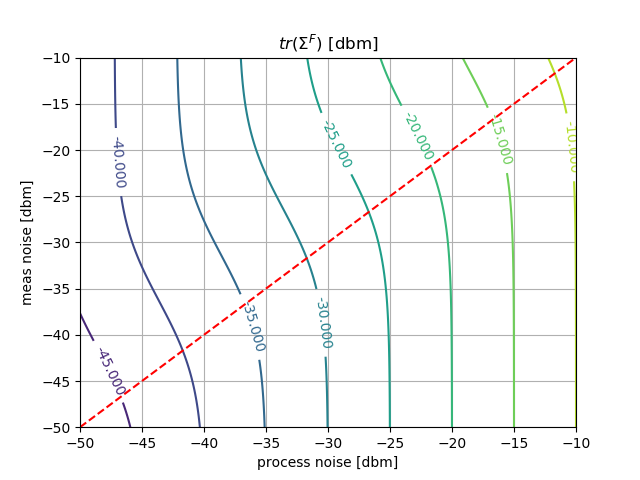
\includegraphics[width=\textwidth]{./fig_1d_filt_f09}
    %\caption{\label{fig:fig_1d_filt_f09}$Filtering, f=0.9$}
  \end{minipage}
  %\hfill
  \begin{minipage}[b]{0.45\textwidth}
    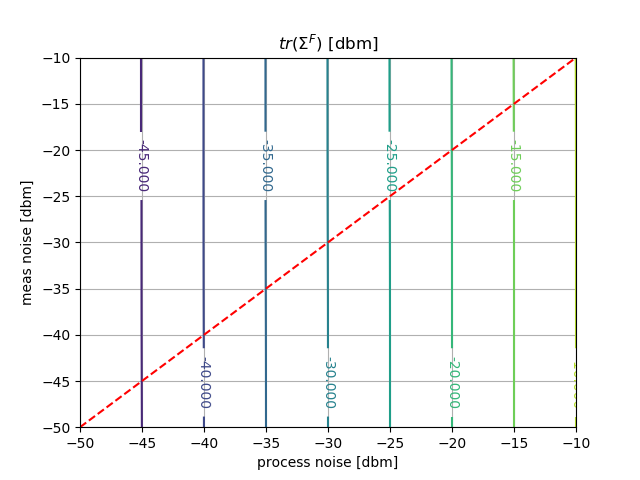
\includegraphics[width=\textwidth]{./fig_1d_filt_f01}
    %\caption{\label{fig:fig_1d_filt_f01}$Filtering, f=0.1$}
  \end{minipage}
  \vfill
  \begin{minipage}[b]{0.45\textwidth}
    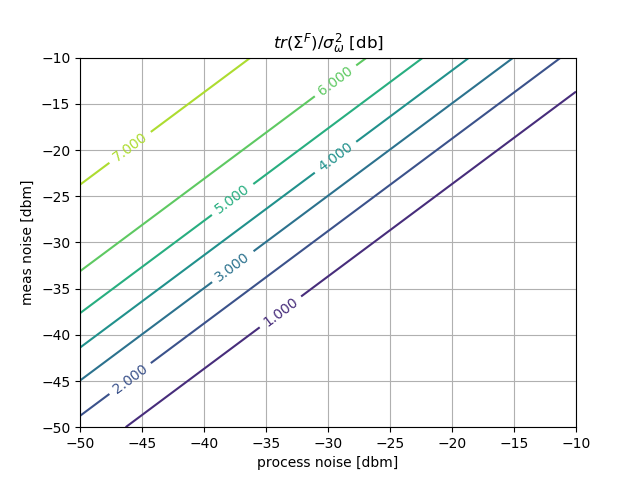
\includegraphics[width=\textwidth]{./fig_1d_filt_f09_wrt_noiseVar}
    %\caption{\label{fig:fig_1d_filt_f01}$Filtering, f=0.1$}
  \end{minipage}  
  \begin{minipage}[b]{0.45\textwidth}
    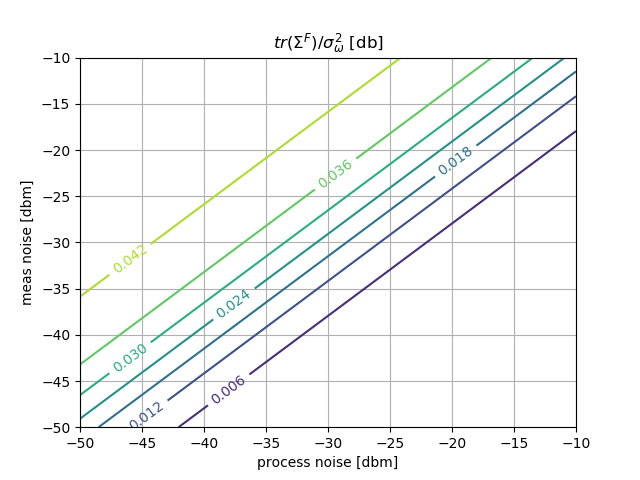
\includegraphics[width=\textwidth]{./fig_1d_filt_f01_wrt_noiseVar}
    %\caption{\label{fig:fig_1d_filt_f01}$Filtering, f=0.1$}
  \end{minipage}   
  \caption{\label{fig:fig_1d_filtering}Filtering estimation error variance - $f=0.9$ left, $f=0.1$ right. Estimation error increases linearly on the line $\sigma_\omega^2=\sigma_v^2$.}
\end{figure}
%
At the limit $f \xrightarrow{} 0$ we have $\Bar{\sigma}_e^2 = \sigma_\omega^2$ (from equation \ref{eq:sigma_bar_1d} or from equation \ref{eq:sigma_bar_1d_constrains}). Notice that for the Kalman gain we also have $\operatorname{lim}_{f \xrightarrow{} 0} K = 0$, therefore the state estimation is constantly zero (assuming the filter was initialized with $x_0=0$) which yields the estimation error $\Bar{\sigma}_e^2 = \sigma_\omega^2$. This result explains the vertical lines seen in figure \ref{fig:component_1_filtering} obtained with parameter value of $f=0.1$.\\\\
%
At the limit $f \xrightarrow{} 1$ we have $\sigma_v^2 = \Bar{\sigma}_e^2(\frac{\Bar{\sigma}_e^2}{\sigma_\omega^2} - 1)$ with $0 < \sigma_\omega^2 < \sigma_e^2$. The Kalman gain is $\operatorname{lim}_{f \xrightarrow{} 1} K = \frac{\Bar{\sigma}_e^2}{\Bar{\sigma}_e^2 + \sigma_v^2}$ and the filter is $\hat{x}_{k+1 \mid k} = \frac{\sigma_v^2}{\Bar{\sigma}_e^2 + \sigma_v^2}\hat{x}_{k \mid k-1} + \frac{\Bar{\sigma}_e^2}{\Bar{\sigma}_e^2 + \sigma_v^2}z_k$. Figure \ref{fig:fig_1d_filtering} depicts equal filtering error variance lines for $f=0.1$ and $f=0.9$.\\\\
%
\subsubsection{Analytic analysis of a single-dimension system at smoothing}
For analyzing the error variance in smoothing we evaluate equation \ref{eq:lin_sigma_smoothing} for the 1d scenario (again, setting $H=1$):
%
\begin{equation}\label{eq:smoothing_imp}
    \begin{split}
        \Bar{\sigma}_e^2 - \sigma_{e,s}^2 &= \frac{\Bar{\sigma}_e^4}{(1 - {\tilde{F}}^2)(\Bar{\sigma}_e^2 + \sigma_v^2)}\\
    \end{split}
\end{equation}
%
Substituting $\tilde{F} = f - K = f - \frac{f\Bar{\sigma}_e^2}{\Bar{\sigma}_e^2 + \sigma_v^2}=f \frac{\Bar{\sigma}_v^2}{\Bar{\sigma}_e^2 + \sigma_v^2}$ we obtain:
%
\begin{equation}\label{eq:filt_smooth_dif}
    \begin{split}
        \Bar{\sigma}_e^2 - \sigma_{e,s}^2 = \Bar{\sigma}_e^4 \frac{\Bar{\sigma}_e^2 + \sigma_v^2}{(\Bar{\sigma}_e^2 + \sigma_v^2)^2 - f^2 \sigma_v^4} > 0\\
        %
        \sigma_{e,s}^2 = \Bar{\sigma}_e^2\left(1 - \Bar{\sigma}_e^2 \frac{\Bar{\sigma}_e^2 + \sigma_v^2}{(\Bar{\sigma}_e^2 + \sigma_v^2)^2 - f^2 \sigma_v^4}\right) > 0\\
    \end{split}
\end{equation}
(both values were verified to be greater than 0).\\
Equal $\sigma_{e,s}^2$ lines seems to have a highly complicated function (substituting equation \ref{eq:sigma_bar_1d} into equation \ref{eq:filt_smooth_dif}). By using the definition of $\eta = \frac{\sigma_v^2}{\sigma_\omega^2}$ and by defining $\Bar{\sigma}_e^2 = 0.5 \sigma_\omega^2\gamma$ with $\gamma = \gamma(f,\eta)$ (thus compressing equation \ref{eq:sigma_bar_1d_eta}) we derive:
%
\begin{equation}\label{eq:smoothing_err}
    \begin{split}
        \sigma_{e,s}^2 = 0.5 \sigma_\omega^2 \left( \gamma - \frac{0.5(0.5\gamma+\eta)\gamma^2}{(0.5\gamma+\eta)^2-f^2\eta^2}\right)
    \end{split}
\end{equation}
%
Some observations:
\begin{equation*}
    \begin{split}
        &\operatorname{lim}_{\eta \xrightarrow{} 0}\sigma_{e,s}^2 = 0\\
        %
        &\sigma_{e,s}^2(\eta=1) = 0.5 \sigma_\omega^2 \left( (f^2+\sqrt{f^4+1}) - \frac{0.5(0.5(f^2+\sqrt{f^4+1})+1)(f^2+\sqrt{f^4+1})^2}{(0.5(f^2+\sqrt{f^4+1})+1)^2-f^2}\right)
    \end{split}
\end{equation*}
%
Figure \ref{fig:sm_vs_fl_different_f} depicts these theoretical $\sigma_{e,s}^2$ and $\Bar{\sigma}_e^2$ for different $f$-values. To verify, we ran simulations which agreed with the theoretical results and are marked by '+' signs in the figure. Figure \ref{fig:fig_1d_smoothing} show smoothing error variances for $f=0.9$ and $f=0.1$.\\\\
%
\begin{figure}
    \centering
        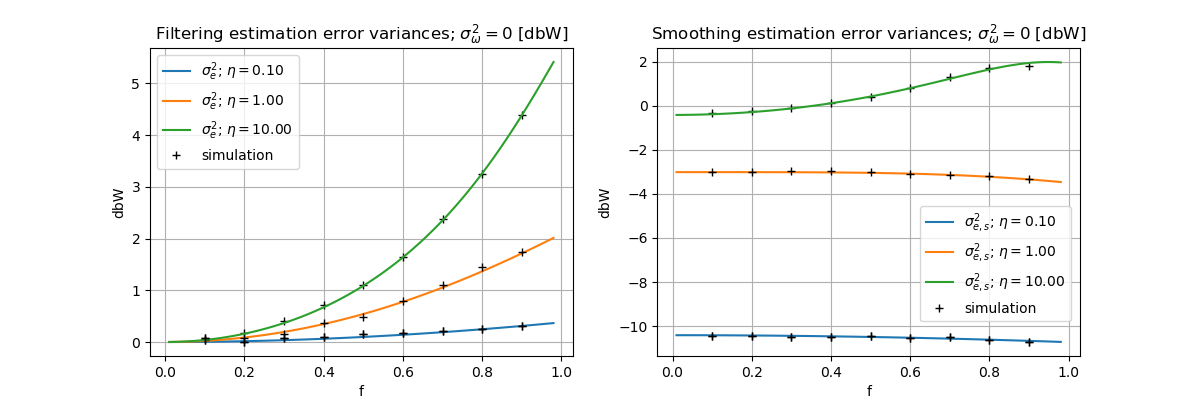
\includegraphics[width=1\textwidth]{./sm_vs_fl_different_f}
        \caption{\label{fig:sm_vs_fl_different_f}Filtering and smoothing estimation error variances}
\end{figure}
%
%
\begin{figure}[!tbp]
  \centering
  \begin{minipage}[b]{0.45\textwidth}
    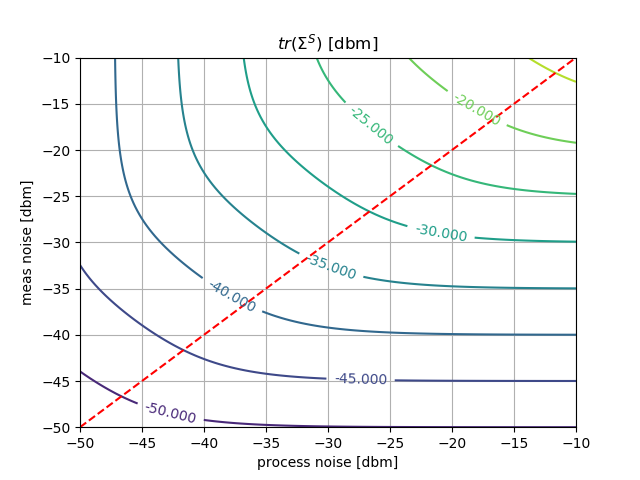
\includegraphics[width=\textwidth]{./fig_1d_smoothing_f09}
    %\caption{\label{fig:fig_1d_smoothing_f09}$Smoothing, f=0.9$}
  \end{minipage}
  %\hfill
  \begin{minipage}[b]{0.45\textwidth}
    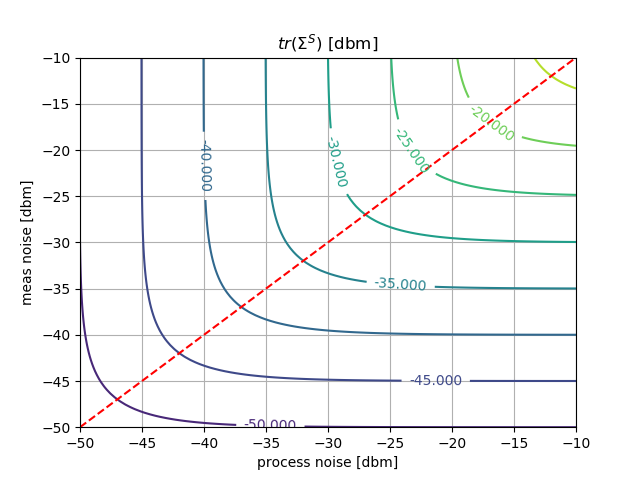
\includegraphics[width=\textwidth]{./fig_1d_smoothing_f01}
    %\caption{\label{fig:fig_1d_smoothing_f01}$Smoothing, f=0.1$}
  \end{minipage}
  \vfill
    \begin{minipage}[b]{0.45\textwidth}
    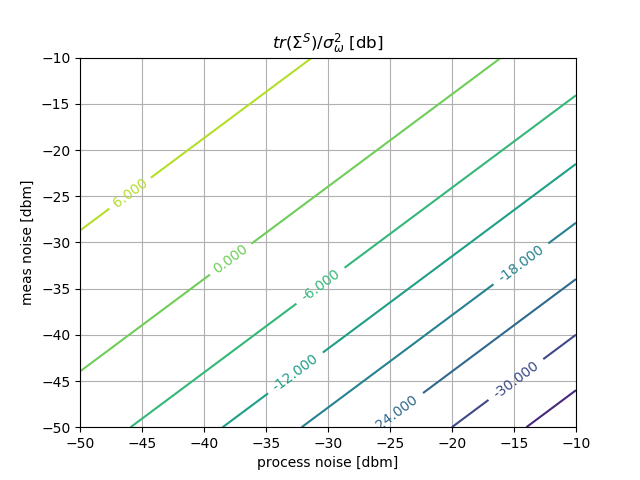
\includegraphics[width=\textwidth]{./fig_1d_smoothing_f09_wrt_noiseVar}
    %\caption{\label{fig:fig_1d_smoothing_f09}$Smoothing, f=0.9$}
  \end{minipage}
  %\hfill
  \begin{minipage}[b]{0.45\textwidth}
    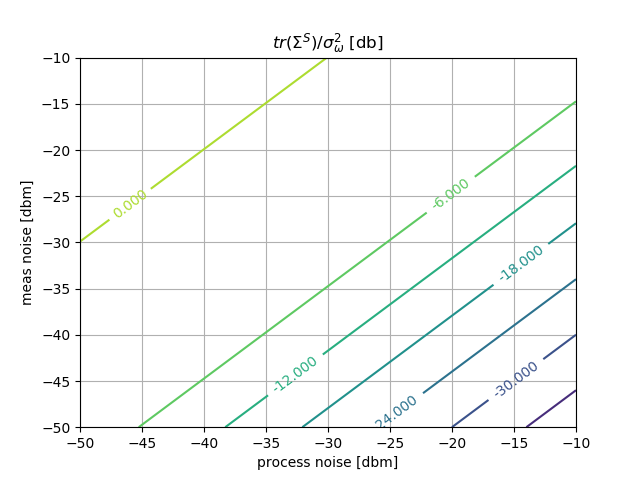
\includegraphics[width=\textwidth]{./fig_1d_smoothing_f01_wrt_noiseVar}
    %\caption{\label{fig:fig_1d_smoothing_f01}$Smoothing, f=0.1$}
  \end{minipage}
  \caption{\label{fig:fig_1d_smoothing}Smoothing estimation error variance - $f=0.9$ left, $f=0.1$ right. Estimation error increases linearly on the line $\sigma_\omega^2=\sigma_v^2$.}
\end{figure}
%
How far into the future do we need to look to see changes from filtering? To answer this question we look at equation \ref{eq:sigma_smoothing} for the 1D scenario:
%
\begin{equation}\label{eq:sigma_smoothing_1d}
    \begin{split}
        \sigma_{j \mid k}^2 &= \Bar{\sigma}_e^2\left(1 - \frac{\Bar{\sigma}_e^2}{\Bar{\sigma}_e^2 + \sigma_v^2} \sum_{i=0}^{k-j} \tilde{F}^{2i}\right) \quad \forall{k>j}\\
        %
        &= \Bar{\sigma}_e^2\left(1 - \frac{\Bar{\sigma}_e^2}{\Bar{\sigma}_e^2 + \sigma_v^2} \frac{1-\tilde{F}^{2(k-j+1)}}{1-\tilde{F}^{2}}\right)
    \end{split}
\end{equation}
%
With $\sigma_{j \mid k}^2$ being the smoothing estimation error variance for estimating the state at time $j$ given observations up to time $k>j$, $\tilde{F} = F - KH' = f \frac{\sigma_v^2}{\Bar{\sigma}_e^2 + \sigma_v^2}$ is the Kalman-filter matrix and the power-series sum formulate is taken from \href{https://en.wikipedia.org/wiki/Geometric_series#Formula}{Wikipedia}. The rate of convergence to $\sigma^2_{j \mid \infty}$ is therefore dependent on the time-constant of the Kalman-filter matrix.
%
\subsubsection{Analytic analysis of filtering vs smoothing for a single-dimension system}
We instead focus on the difference between filtering and smoothing. From equation \ref{eq:filt_smooth_dif} and using the definition of equation \ref{eq:f_vs_s_def} we can deduce:
%
\begin{equation}
    \begin{split}
        \psi_{FS} = \frac{\Bar{\sigma}_e^2 \frac{\Bar{\sigma}_e^2 + \sigma_v^2}{(\Bar{\sigma}_e^2 + \sigma_v^2)^2 - f^2 \sigma_v^4}}{1 - 0.5\Bar{\sigma}_e^2 \frac{\Bar{\sigma}_e^2 + \sigma_v^2}{(\Bar{\sigma}_e^2 + \sigma_v^2)^2 - f^2 \sigma_v^4}}\\
    \end{split}
\end{equation}
%
By using the definition of $\eta = \frac{\sigma_v^2}{\sigma_\omega^2}$ and by defining $\Bar{\sigma}_e^2 = 0.5 \sigma_\omega^2\gamma$ with $\gamma = \gamma(f,\eta)$ we derive:
%
\begin{equation}\label{eq:deltaFs}
    \begin{split}
        \psi_{FS} = \frac{\gamma \frac{0.5\gamma + \eta}{(0.5\gamma + \eta)^2 - f^2 \eta^2}}{2 - 0.5\gamma \frac{0.5\gamma + \eta}{(0.5\gamma + \eta)^2 - f^2 \eta^2}} 
    \end{split}
\end{equation}
According to equation \ref{eq:deltaFs}, $\psi_{FS}$ is a function only of the noises ratio $\eta$ and the dynamics $f$. Therefore, for a fixed $f$ value, equal valued $\psi_{FS}$ lines are linear. It is easily seen that $\operatorname{lim}_{\eta \xrightarrow{} 0}\psi_{FS} = 2$ which is in agreement with previous results. For different $\eta$ values the dependents of $\psi_{FS}$ on $f$ is depicted in figure \ref{fig:deltaFS_vs_f}.\\\\
%
\begin{figure}
    \centering
        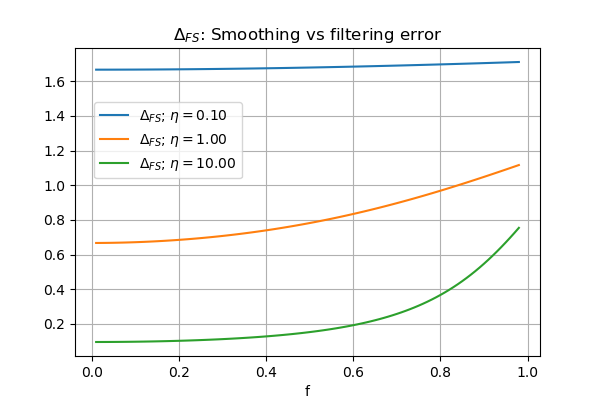
\includegraphics[width=0.8\textwidth]{./deltaFS_vs_f}
        \caption{\label{fig:deltaFS_vs_f}$\psi_{FS}$ for different $\eta$ values}
\end{figure}
%
Equal valued $\psi_{FS}$ lines are:
%
\begin{equation}\label{eq:deltaFS_eq}
    \begin{split}
        0.5\gamma \frac{0.5\gamma + \eta}{(0.5\gamma + \eta)^2 - f^2 \eta^2} -c' &= 0
    \end{split}
\end{equation}
%
With $c' = \frac{\psi_{FS}}{1+0.5\psi_{FS}}$.\\\\
%
%
According to equation \ref{eq:deltaFS_eq} the equal valued $\psi_{FS}$ lines are of course also a function only of the noises ratio $\eta$ and the dynamics $f$.\\\\ %If these equal valued lines are linear in the $(\sigma_v^2,\sigma_\omega^2)$ plane then differentiating equation \ref{eq:deltaFS_eq} with respect to $\sigma_v^2$ and $\sigma_\omega^2$ should yield constant values.\\
For $f \xrightarrow{} 0$, we showed that $\Bar{\sigma}_e^2 = \sigma_w^2$, the equal lines are:
%
\begin{equation}
    \begin{split}
        \sigma_v^2 &= \left( \psi_{FS}^{-1}-0.5 \right)\sigma_\omega^2
    \end{split}
\end{equation}
%
For $f \xrightarrow{} 1$ the equal lines are:
\begin{equation}\label{eq:lin_f_1}
    \begin{split}
        \sigma_v^2 &= \frac{1+c''}{{c''}^2}\sigma_w^2\\
        c'' &= \frac{3\psi_{FS}-2}{2-\psi_{FS}}
    \end{split}
\end{equation}
%
\subsubsection{Filtering vs smoothing - conclusions}
We analytically analyzed the behaviour of filtering and smoothing for a single dimension scenario:
%
\begin{equation}\label{eq:kalmanModel_1d}
    \begin{split}
        x_{k+1} &= fx_k + \omega_k\\
        z_k &= x_k + v_k
    \end{split}
\end{equation}
%
$\{\omega_k\}$, $\{v_k\}$, $\{x_0\}$ are independent white Gaussian processes,
%
\begin{equation*}
    \operatorname{E} \begin{bmatrix} \begin{bmatrix} \omega_k \\ v_k \end{bmatrix} &  \begin{bmatrix} \omega_l' & v_l' \end{bmatrix} \end{bmatrix} = \begin{bmatrix} \sigma_\omega^2 & 0 \\ 0 & \sigma_v^2\end{bmatrix} \psi_{kl}
\end{equation*}
%
and $\abs{f}<1$. The behaviour is a function of the dynamics $f$, the process noise $\sigma_\omega^2$ and the measurement noise $\sigma_v^2$. The ratio of both filtering and smoothing errors to the process noise is a function of the dynamics and the ratio $\eta = \frac{\sigma_v^2}{\sigma_\omega^2}$ (equations \ref{eq:sigma_bar_1d_eta}, \ref{eq:smoothing_err}). Therefore, without loss of generality we set $\sigma_\omega^2=1$ and analyze the system with respect to $f$ and $\eta$. The main conclusions are:
%
\begin{itemize}
    \item Filtering error variance is always higher than the process noise.
    %
    \item Filtering error variance ןincreases with $f$ (and of course also with $\eta$).
    %
    \item Smoothing error variance can reach zero for low measurement noise.
    %
    \item Smoothing error variance is less sensitive to $f$. Depending on $\eta$ it either increases or decreases with $f$. There seems to be a value $\eta^*$ for which smoothing error variance is independent of $f$.
    %
    \item In equation \ref{eq:f_vs_s_def} we defined $\psi_{FS}$ as filtering vs smoothing error comparison. We showed it to be dependent on $f$ and $\eta$ alone.  
\end{itemize}
%
Figure \ref{fig:conclusions} summaries all the results obtained. Different values of $\sigma_\omega^2$ would only change the values of the contours seen, but not their shapes. 
%
\begin{figure}
    \centering
        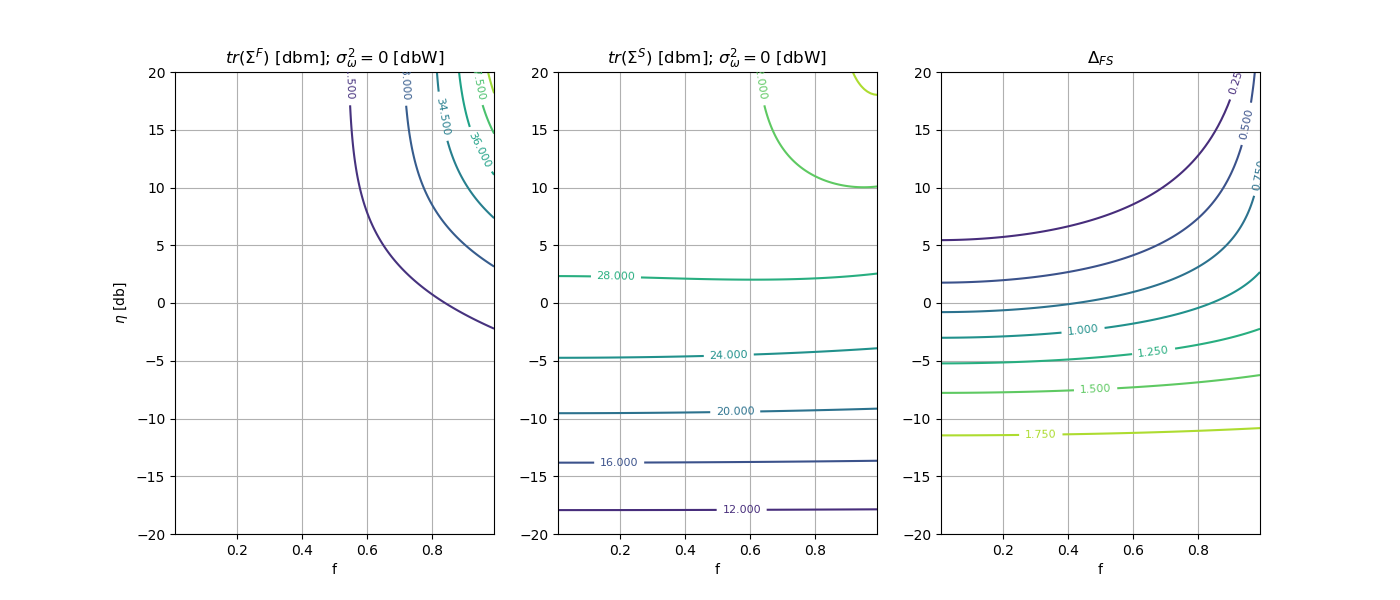
\includegraphics[width=1.0\textwidth]{./conclusions}
        \caption{\label{fig:conclusions}Summary of filtering and smoothing errors. Different values of $\sigma_\omega^2$ would only change the values of the contours seen, but not their shapes.}
\end{figure}
%
\subsubsection{Simulation of unmodeled behaviour (17.04)}
We would like to simulate filtering and smoothing estimation errors for measurements that contain an unmodeled behaviour which is correlated with the dynamics of the modeled part of the system.
While the model by which the filter and the smoother operate is that given in equation \ref{eq:kalmanModel_1d} the true system-sensor behaviour is given by:
%
\begin{equation}\label{eq:kalman_1d_unmodeled}
    \begin{split}
        &x^{(1)}_{k+1} = fx^{(1)}_k + \omega_k\\
        &x^{(2)}_{k} = x^{(1)}_{k} + \alpha\operatorname{sin}(2\pi f \frac{k}{f_s} + \phi_0)\\
        &z_k = x^{(2)}_k + v_k
    \end{split}
\end{equation}
%
With $\phi_0 \sim U[0, 2\pi]$, $f_s = 10$ and $\alpha$ controls the power ratio between the unmodeled behaviour $\operatorname{sin}(2\pi f \frac{k+1}{f_s} + \phi_0)$ and the modeled behaviour $x^{(1)}_{k}$. As before $\{\omega_k\}$, $\{v_k\}$, $\{x_0\}$ are independent white Gaussian processes,
%
\begin{equation*}
    \operatorname{E} \begin{bmatrix} \begin{bmatrix} \omega_k \\ v_k \end{bmatrix} &  \begin{bmatrix} \omega_l' & v_l' \end{bmatrix} \end{bmatrix} = \begin{bmatrix} \sigma_\omega^2 & 0 \\ 0 & \sigma_v^2\end{bmatrix} \psi_{kl}
\end{equation*}
%
and $\abs{f}<1$. Figure \ref{fig:unmodeledBehaviour} shows that for $\alpha=0.75$ smoothing obtains smaller estimation errors. 
%
\begin{figure}
    \centering
        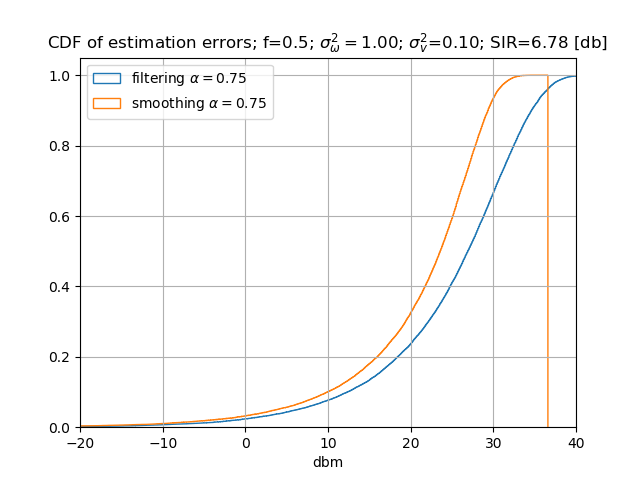
\includegraphics[width=0.8\textwidth]{./unmodeledBehaviour}
        \caption{\label{fig:unmodeledBehaviour}CDF of estimation errors collected from 10 independent simulations. On average, smoothing estimation errors are 3.6 [db] lower than filtering estimation errors. With $\alpha=0.75$, $f=0.5$ and $\sigma_\omega^2=1$ we have a power ratio of 6.78 [db] between the modeled and unmodeled parts of the state $x^{(2)}$.}
\end{figure}
%
\subsubsection{Example (20.03)}
We analyze the next specific dynamics for different process and measurement noises.
\begin{equation}
    \begin{split}
        F &= \begin{bmatrix} \beta & 0 \\ dt & \alpha \end{bmatrix}\\
        H' &= \begin{bmatrix} 1 & 0\end{bmatrix}\\
        \omega_k &= \begin{bmatrix} w_k^i \\ 0 \end{bmatrix}\\
        w_k^i &\sim \operatorname{N}(0, \sigma_\omega^2)\\
        v_k &\sim \operatorname{N}(0, \sigma_v^2)\\
    \end{split}
\end{equation}
%
With $\alpha = 0.9$, $\beta = 0.1$ and $dt=0.5$. The errors of filtering, smoothing and a comparison between them according to the definition of eq. \ref{eq:f_vs_s_def} is shown in figures \ref{fig:Filtering_meas_a}, \ref{fig:Smoothing_meas_a}, \ref{fig:Filtering_vs_Smoothing_meas_a}.
%
\begin{figure}
    \centering
        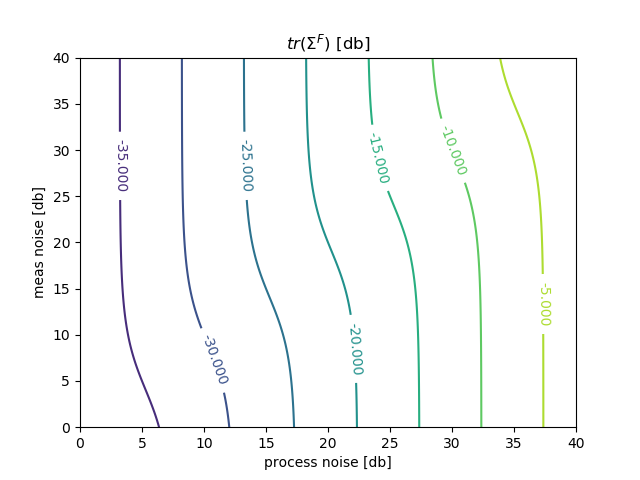
\includegraphics[width=0.8\textwidth]{./Filtering_meas_a}
        \caption{\label{fig:Filtering_meas_a}Trace of error covariance matrix for filtering}
\end{figure}
%
%
\begin{figure}
    \centering
        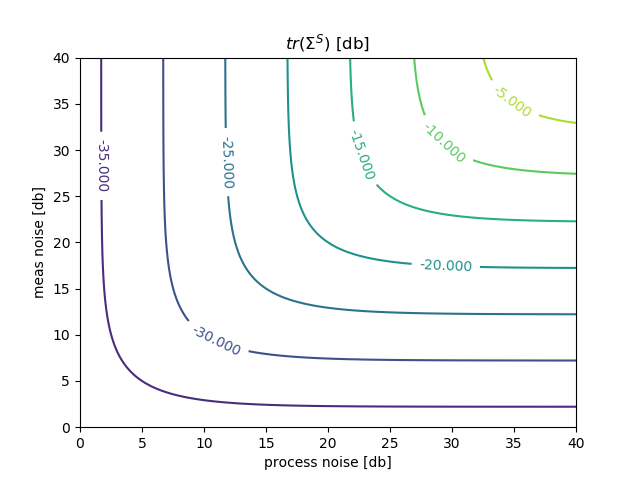
\includegraphics[width=0.8\textwidth]{./Smoothing_meas_a}
        \caption{\label{fig:Smoothing_meas_a}Trace of error covariance matrix for smoothing}
\end{figure}
%
%
\begin{figure}
    \centering
        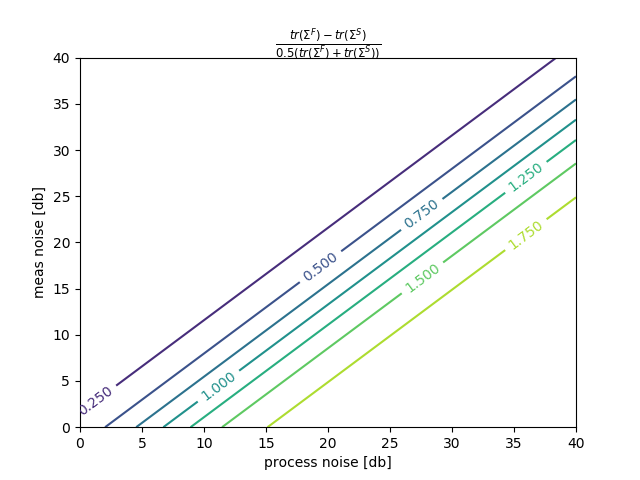
\includegraphics[width=0.8\textwidth]{./Filtering_vs_Smoothing_meas_a}
        \caption{\label{fig:Filtering_vs_Smoothing_meas_a}Filtering vs smoothing according to the definition of eq. \ref{eq:f_vs_s_def}}
\end{figure}
%
\\\\Notes on the results in this example:
\begin{itemize}
    \item Filtering mostly gains from a decrease in the processing noise
    \item Smoothing has a symmetry axis which in figure \ref{fig:Smoothing_meas_a} is about the $45^o$ axis. Below this axis smoothing error performance is not sensitive to changes in processing noise while above the axis it is not sensitive to changes in sensor noise. 
    \item There are equal filtering-vs-smoothing lines, at about $45^o$. Smoothing increases its advantage when measurement noise decreases but decreases its advantage when processing noise decreases. 
\end{itemize}
%
Analyzing each component separately. The first component in figures \ref{fig:component_1_filtering} - \ref{fig:component_1_delta}, the second component in figures \ref{fig:component_2_filtering} - \ref{fig:component_2_delta}.
%
%
\begin{figure}
    \centering
        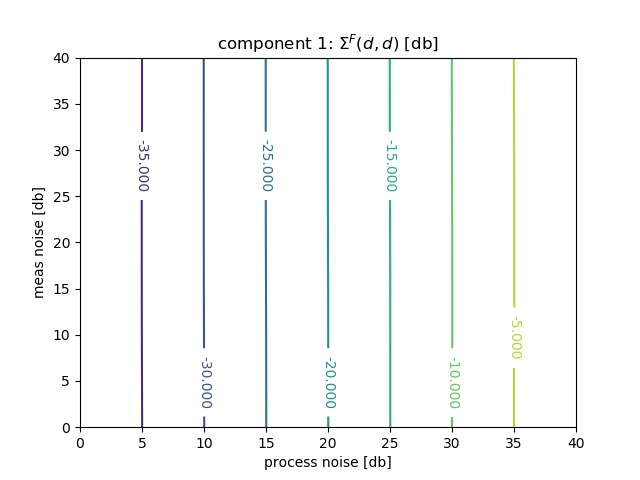
\includegraphics[width=0.8\textwidth]{./component_1_filtering}
        \caption{\label{fig:component_1_filtering}Error of first component for filtering}
\end{figure}
%
%
\begin{figure}
    \centering
        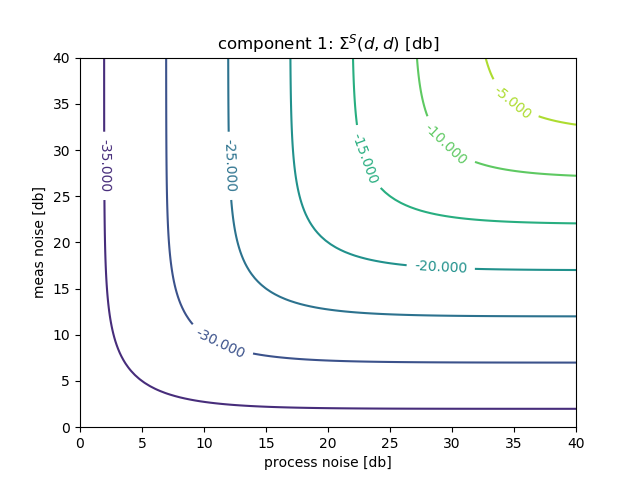
\includegraphics[width=0.8\textwidth]{./component_1_smoothing}
        \caption{\label{fig:component_1_smoothing}Error of first component for smoothing}
\end{figure}
%
%
\begin{figure}
    \centering
        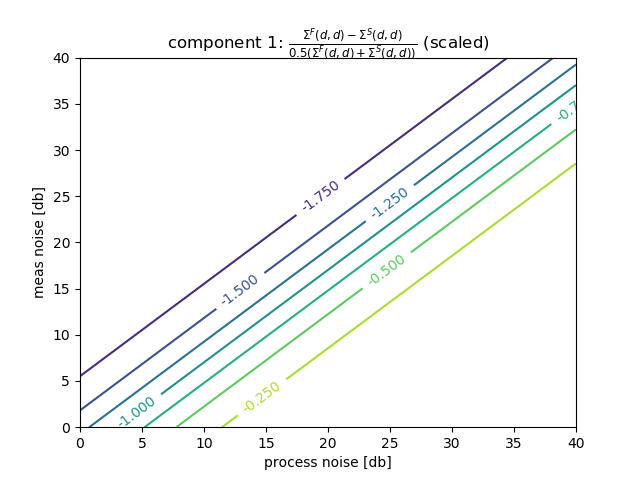
\includegraphics[width=0.8\textwidth]{./component_1_delta}
        \caption{\label{fig:component_1_delta}First component Filtering vs smoothing according to the definition of eq. \ref{eq:f_vs_s_def}}
\end{figure}
%
%
\begin{figure}
    \centering
        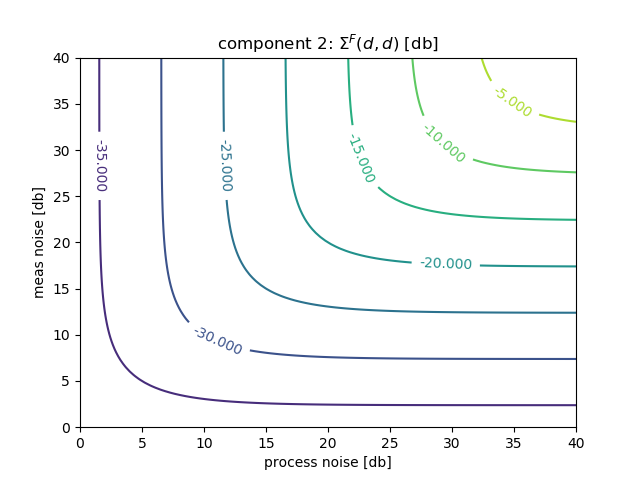
\includegraphics[width=0.8\textwidth]{./component_2_filtering}
        \caption{\label{fig:component_2_filtering}Error of second component for filtering}
\end{figure}
%
%
\begin{figure}
    \centering
        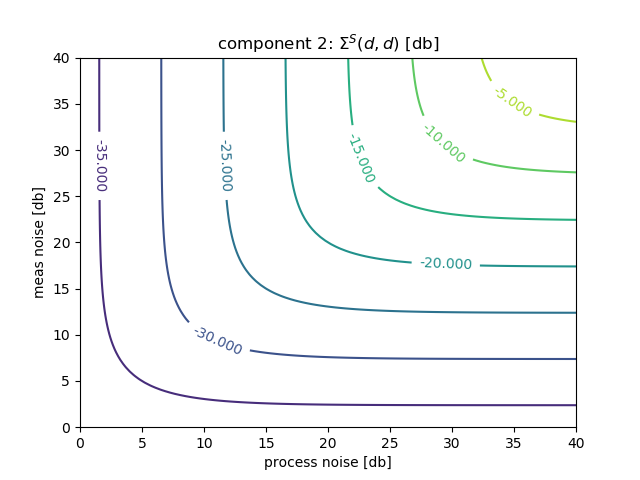
\includegraphics[width=0.8\textwidth]{./component_2_smoothing}
        \caption{\label{fig:component_2_smoothing}Error of second component for smoothing}
\end{figure}
%
%
\begin{figure}
    \centering
        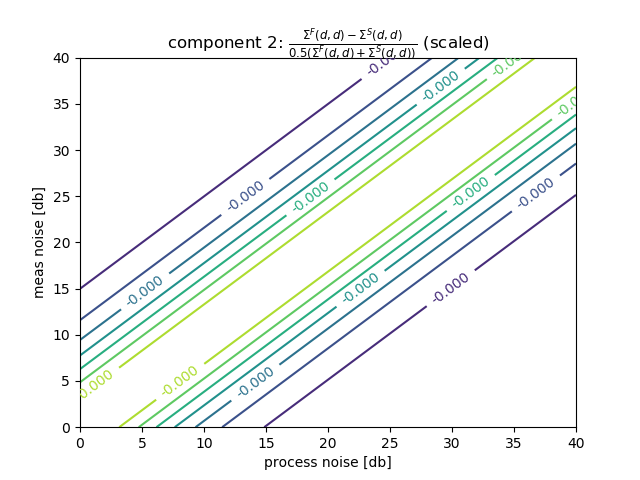
\includegraphics[width=0.8\textwidth]{./component_2_delta}
        \caption{\label{fig:component_2_delta}Second component Filtering vs smoothing according to the definition of eq. \ref{eq:f_vs_s_def}}
\end{figure}
%
\subsection{HMM (29.02)}
Notations:
\begin{itemize}
    \item $h_t$ - hidden state at time $t$ 
    \item $v_t$ - observation at time $t>0$; $v_{t_1:t_2}$ - observations from time $t_1$ to time $t_2$
    \item $\alpha(h_t) = p(h_t, v_{1:t})$, $\beta(h_t) = p(v_{t+1:T} \mid h_t)$, $\gamma(h_t) = p(h_t, v_{1:T})$\\$h_t$ can take one of $S$ discrete states
    \item $P^v_t = \operatorname{diag}\left(\begin{bmatrix} p(v_t \mid h_t=1), \ldots , p(v_t \mid h_t=S) \end{bmatrix}\right)$ - diagonal matrix of the likelihood of observation $v_t$ with respect to each possible state
    \item $A$ - transition probability matrix of size $[S \times S]$; $A[r,c]=p(h_{t+1}=r \mid h_t=c) \quad \forall{t}$
    \item $\alpha_t = \begin{bmatrix} \alpha(h_t=1)& \cdots &\alpha(h_t=S) \end{bmatrix}^T$, $\beta_t = \begin{bmatrix} \beta(h_t=1)& \cdots &\beta(h_t=S) \end{bmatrix}^T$\\$\gamma_t = \begin{bmatrix} \gamma(h_t=1)& \cdots &\gamma(h_t=S) \end{bmatrix}^T$
    \item $d_{[S \times 1]} = \begin{bmatrix} 1& \cdots& 1\end{bmatrix}^T$
\end{itemize}
\\%
\underline{Filtering recursion} \cite{barber2012bayesian}:
\begin{equation}\label{eq:filteringRecursion}
    \alpha(h_t) = p(v_t \mid h_t) \sum_{h_{t-1}} p(h_t \mid h_{t-1}) \alpha(h_{t-1})\quad t>1
\end{equation}
%
With $\alpha(h_1) = p(v_1 \mid h_1)p(h_1)$.\\
In a discrete Hidden Markov Model (HMM) $h_t$ can take one of $S$ discrete states; $A_{[S \times S]}$ is the transition probability matrix. We can state the recursion in matrix form as:
%
\begin{equation}\label{eq:filteringRecursion_matrix}
    \alpha_t = P^v_t A \alpha_{t-1} = \left(\prod_{\tau=2}^t P^v_\tau A\right)\alpha_1 \quad t>1
\end{equation}
%
With $\alpha_1 = P^v_1 d$ when assuming a uniform prior on the states.\\\\
\underline{Parallel smoothing recursion}:\\
For smoothing estimation we would like to derive an expression for $p(h_t, v_{1:T})$:
\begin{equation}\label{eq:par_smoothing}
    \gamma(h_t) = p(h_t, v_{1:T}) = p(h_t, v_{1:t}, v_{t+1:T}) = p(h_t, v_{1:t}) p(v_{t+1:T} \mid h_t, \hcancel{v_{1:t}}) = \alpha(h_t) \beta(h_t) 
\end{equation}
%
A recursion for $\beta(h_t)$:
\begin{equation}\label{eq:beta_rec}
    \beta(h_t) = \sum_{h_{t+1}} p(v_{t+1} \mid h_{t+1}) p(h_{t+1} \mid h_t) \beta(h_{t+1})
\end{equation}
%
We can state the recursion in matrix form as:
%
\begin{equation}\label{eq:beta_matrix}
    \beta_t = A^T P^v_{t+1} \beta_{t+1} = \left( \prod_{\tau=T-1}^t A^T P^v_{\tau+1}\right) \beta_T
\end{equation}
%
With $\beta_T = \operatorname{ones}(S \times 1)$. We can state $\gamma_t$ in a matrix form as:
\begin{equation}\label{eq:gamma_mat}
    \gamma_t = \operatorname{diag}(\alpha_t) \beta_t
\end{equation}
%
Let us analyze a simple case of two observations, $v_{1:2}$, in which we would like an estimation for $h_1$.
%
\begin{equation}\label{eq:two_obs}
    \begin{split}
        \alpha_1 &= P^v_1 d\\
        \beta_1 &= A^T P^v_{2} \beta_2 = A^T P^v_{2} d\\
        \gamma_1 &= \operatorname{diag}(\alpha_1) \beta_1 = \operatorname{diag}(P^v_1 d) A^T P^v_{2} d = P^v_1 A^T P^v_{2} d
    \end{split}
\end{equation}
%
To obtain filtering and smoothing probabilities we must normalize $\alpha_t$ and $\gamma_t$:
\begin{equation}\label{eq:norm_probs}
    \begin{split}
        \begin{bmatrix} p(h_t=1 \mid v_{1:t})& \cdots& p(h_t=S \mid v_{1:t}) \end{bmatrix}^T &= \frac{1}{\sum \alpha_t}\alpha_t = \frac{1}{d^T\alpha_t} \alpha_t\\
        %
        \begin{bmatrix} p(h_t=1 \mid v_{1:T})& \cdots& p(h_t=S \mid v_{1:T}) \end{bmatrix}^T &= \frac{1}{\sum \gamma_t}\gamma_t = \frac{1}{d^T\gamma_t} \gamma_t
    \end{split}
\end{equation}
%
With $d_{[S \times 1]} = \begin{bmatrix} 1& \cdots& 1\end{bmatrix}^T$.\\\\
%
Without loss of generality we assume that at time $t=1$ the state is $h_t=1$.\\We would like to obtain constrains on $P^v_1$, $P^v_2$ and $A$ so that $p(h_1=1 \mid v_{1}) \leq p(h_1=1 \mid v_{1:2})$:
%
\begin{equation}\label{eq:f_vs_s}
    \begin{split}
        p(h_1=1 \mid v_{1}) &\leq p(h_1=1 \mid v_{1:2})\\
        %
        \frac{e_1^T\alpha_1}{d^T\alpha_1} &\leq \frac{e_1^T\gamma_1}{d^T\gamma_1}\\
        %
        \frac{e_1^T P^v_1 d}{d^T P^v_1 d} &\leq \frac{e_1^T P^v_1 A^T P^v_{2} d}{d^T P^v_1 A^T P^v_{2} d}\\
    \end{split}
\end{equation}
%
With $e_1 = \begin{bmatrix} 1& 0 & \cdots& 0 \end{bmatrix}^T$ - $[S \times 1]$ vector.
%
%
\section{Formalization of radar scenario (28.04)}\label{sec:Radar_problem}
%
In the radar scenario we would like to continuously estimate (i.e. track) the range $d(t)$ with respect to a moving target. The radar continuously transmits pulses $u(t)$ and receives echos $y(t)$ returned from the target. The measurement $z(t)$ is the inner product between the received signal and the transmitted pulse with additive noise. We begin by writing in equation \ref{eq:target} the model equations for the target, for simplicity we assume a ballistic target with acceleration $a(t)$ affected by a gravitation force $F_G$ and noise-wind $\omega_a(t)$:
%
\begin{equation}\label{eq:target}
    \begin{split}
        &\dot{a}(t) = \omega_a(t)\\
        &\dot{v}(t) = a(t) + {\begin{bmatrix} 0 & 0 & F_G \end{bmatrix}}'\\
        &\dot{l}(t) = v(t)\\
    \end{split}
\end{equation}
%
The target equations can be written in a compact form:
%
\begin{equation}\label{eq:target_mat}
    \begin{split}
        \dot{x}(t) = Fx(t) + b + \omega(t)
    \end{split}
\end{equation}
%
with:
%
\begin{equation}\label{eq:target_mat}
    \begin{split}
        &x(t) = {\begin{bmatrix} a(t) & v(t) & l(t) \end{bmatrix}}'\\
        %
        &b = {\begin{bmatrix} 0_{1 \times 5} & F_G & 0_{1 \times 3} \end{bmatrix}}'\\
        %
        &\omega_t(t) = {\begin{bmatrix} \omega_a(t)' & 0_{1 \times 6} \end{bmatrix}}'\\
        %
        %&F = \begin{bmatrix} 
        %0 & 0 & 0 & 0 & 0 & 0 & 0 & 0 & 0 \\
        %0 & 0 & 0 & 0 & 0 & 0 & 0 & 0 & 0 \\
        %0 & 0 & 0 & 0 & 0 & 0 & 0 & 0 & 0 \\
        %
        %1 & 0 & 0 & 0 & 0 & 0 & 0 & 0 & 0 \\
        %0 & 1 & 0 & 0 & 0 & 0 & 0 & 0 & 0 \\
        %0 & 0 & 1 & 0 & 0 & 0 & 0 & 0 & 0 \\
        %
        %0 & 0 & 0 & 1 & 0 & 0 & 0 & 0 & 0 \\
        %0 & 0 & 0 & 0 & 1 & 0 & 0 & 0 & 0 \\
        %0 & 0 & 0 & 0 & 0 & 1 & 0 & 0 & 0 \\
        %\end{bmatrix}\\
        %
        &F = \begin{bmatrix} 
        0_{3 \times 9}\\
        I_{6 \times 6} & 0_{6 \times 3}
        \end{bmatrix}\\
    \end{split}
\end{equation}
%
The measurement equation is:
%
\begin{equation}\label{eq:radar_meas}
    z(t) = \langle g, y(t) + v(t) \rangle = \int_{0}^{T_P} y(\tau + t - T_P) g(\tau) d\tau + \int_{0}^{T_P} v(\tau + t - T_P) g(\tau) d\tau
\end{equation}
%
with $g(0 \leq t < T_P)$ being the transmitted pulse, $y(t)$ the received signal and $v(t)$ additive measurement noise. We now link between the target location and the received signal. First we write the transmitted signal $u(t)$ as a series of pulses with a repetition interval $T_c$:
%
\begin{equation}
    \begin{split}
        &g_{c}(0 \leq t < T_P) = g(t); \quad g_{c}(T_P \leq t < T_c) = 0\\
        %
        &u(t) = g_{c}(t \text{ mod } T_c) 
        %
    \end{split}
\end{equation}
%
In the following equations $f_c$ is the carrier-frequency, $c$ is the speed-of-light, $\sigma_R$ is the unknown Radar-Cross-Section for the target, $\eta(t)$ is the round trip attenuation factor, $d(t)$ is the radar-target range and $\tau(t)$ is the corresponding round trip delay. Without lost of generality we assume the radar is located at the origin.
%
\begin{equation}\label{eq:Rx}
    \begin{split}
        &L = \begin{bmatrix} 0_{3 \times 6} & I_{3 \times 3} \end{bmatrix}\\
        %
        &d(t) = \norm{L x(t)}\\
        %
        &\eta(t) = \frac{c}{8 \pi f_c \sigma_R}\frac{1}{d(t)}\\
        %
        &\tau(t) = 2\frac{d(t)}{c}\\
        %
        &y(t) = \eta(t) u(t - \tau(t))
    \end{split}
\end{equation}
%
Writing $y(t)$ in terms of the estimation objective $d(t)$ we obtain:
%
\begin{equation}\label{eq:radar_rx}
    y(t) = \frac{c}{8 \pi f_c \sigma_R }\frac{1}{d(t)} u(t - \frac{d(t)}{c})
\end{equation}
%
Equations \ref{eq:target_mat}-\ref{eq:radar_rx} describe a system with input $u(t)$, process-noise $\omega(t)$, measurement-noise $v(t)$ and sensor-measurement $z(t)$ as depicted in figure \ref{fig:Radar_diagram}. Our approximated believe for the system's model $\tilde{f}$ and our sensor $h$ are clearly separated at the block diagram.\\\\
%
\begin{figure}
    \centering
        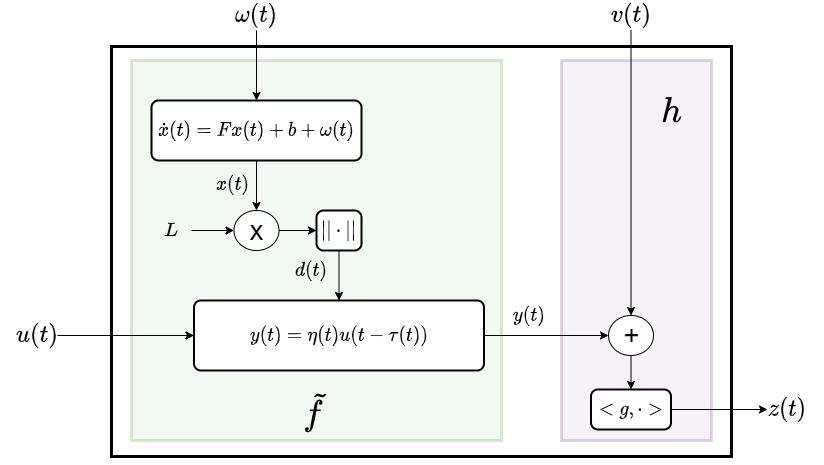
\includegraphics[width=0.9\textwidth]{./Radar_diagram}
        \caption{\label{fig:Radar_diagram}Block-diagram for approximated radar equations}
\end{figure}
%
Range estimations from the measurements $z(t)$ have ambiguities. This is due to the periodic nature of $y(t)$ that results in a periodic nature of $z(t)$:
%
\begin{equation}\label{eq:range_amb}
    \begin{split}
        y(t + kT_c) &= \eta(t + kT_c) u(t + kT_c - \tau(t + kT_c))\\
        %
        &= \eta(t + kT_c) g_{c}(t + kT_c - \tau(t + kT_c) \text{ mod } T_c)\\
        %
        &\approx \eta(t) g_{c}(t - \tau(t) \text{ mod } T_c) = y(t)\\
    \end{split}
\end{equation}
%
The last approximation is due to engineering analysis: pulse repetition interval, $T_c$ is in the order of $30\mu s$ and the relative velocity of the target is in the order of $V_c=100 m/s$. Therefore:
%
\begin{equation}
    \tau(t+kT_c) - \tau(t)=\frac{d(t+kT_c)-d(t)}{c}=\frac{kT_c V_c}{c}=\frac{k}{100}\operatorname{ns}    
\end{equation}
%
We see that even for large values of $k$ the difference in $\tau(t)$ is less than $1 \operatorname{ns}$ and therefore neglectable. The attenuation $\eta(t)$ has neglectable differences due to similar reasons. The obtained measurement $z(t)$ is periodic up to differences that are due to measurement noise:
%
\begin{equation}\label{eq:range_amb}
    \begin{split}
        z(t + kT_c) &= \langle g, y(t + kT_c) + v(t + kT_c) \rangle\\
        %
        &\approx \langle g, y(t) + v(t + kT_c) \rangle\\
        %
        &= z(t) + \langle g, v(t + kT_c) - v(t) \rangle
    \end{split}
\end{equation}
%
The periodicity of the measurements yields ambiguities in the range estimation. To address this problem the radar changes the input $u(t)$ to a batch of pulses with a different pulse repetition interval $T_c'$. The new obtained range estimations have range ambiguities proportional to $T_c'$. Using integer optimization methods the two (or more) sets of estimations are fused and an unambiguous estimation is obtained.\\\\
%
To conclude, we witness a system for which the initial `diagnosis' results in a number of possible  hypotheses. A series of interventions (the input $u(t)$) decreases the likelihood of the wrong  hypotheses.\\\\
%
This model-based estimation process is based on the approximated system model $\tilde{f}$ that assumes that only a single, line-of-sight ray is receipted by the radar. In reality, a fixed stationed radar is influenced by the geographic environment. Assume there is a reflector (a building for example) located at $l_r$. The radar will now receipt a ray that was reflected by the target and then by the reflector in addition to the line-of-sight ray. The additional ray result in a change to $y(t)$ from equation \ref{eq:Rx} that will take the form:
%
\begin{equation}
    y_r(t) = \eta(t) u(t-\tau(t)) + \eta_r(t) u(t-\tau_r(t))
\end{equation}
%
Generalizing for $N_r$ reflectors we derive
%
\begin{equation}\label{eq:y_r}
    y_r(t) = y(t) + \sum_{r=1}^{N_r} \eta_r(t) u(t-\tau_r(t)) = \sum_{r=0}^{N_r} \eta_r(t) u(t-\tau_r(t))
\end{equation}
%
with $\eta_0(t)$ and $\tau_0(t)$ corresponding to the direct line-of-sight reflection; $\eta_r(t),\tau_r(t)$ are all functions of $d(t)$. Figure \ref{fig:Radar-True} shows the correct yet unknown system-sensor model.
%
\begin{figure}
    \centering
        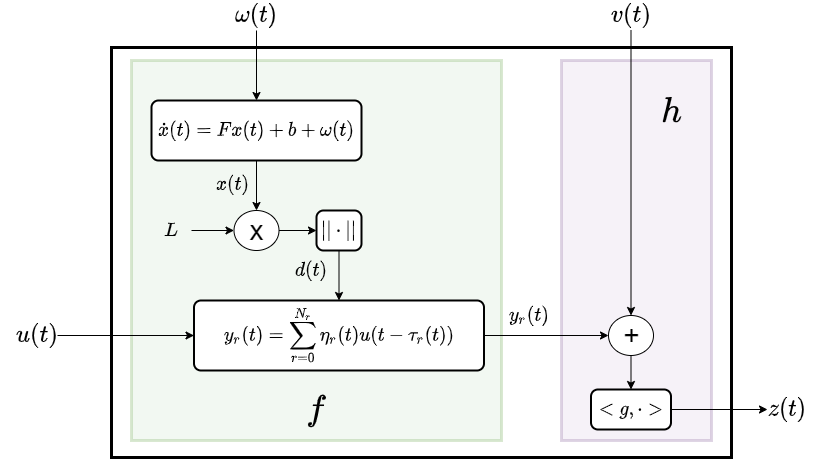
\includegraphics[width=0.9\textwidth]{./Radar-True}
        \caption{\label{fig:Radar-True}Block-diagram for true radar equations}
\end{figure}
%
A few notes on the model ${f}$:
\begin{itemize}
    \item The dominant (power-wise) reflect is the line-of-sight reflect , therefore for all $r>1$ we have that $\abs{\eta_0(t)} > \abs{\eta_r(t)}$.
    \item $\eta_r(t)$ can take negative values due to phase shifts as part of reflections.
    \item The power-envelope of the measurements obtained from $f$ and $\tilde{f}$ is similar. The differences are in fine details of the shape of the returned pulses.
    \item The output $y_r(t)$ from the true-system $f$ is the sum of the output $y(t)$ from the approximated system $\tilde{f}$ and an additional term that is a function of the estimation objective $d(t)$ (as in the example described in equation \ref{eq:kalman_1d_unmodeled}).
\end{itemize}
%
\section{Research objective (03.05)}\label{sec:F_vs_S}
%
In this section we define a research motivated by the radar scenario. In the radar scenario a number of batches of pulses are transmitted, each batch has a different pulse-repetition-interval $T_c(i)$. Using the notations of figure \ref{fig:Radar-True} we say we introduce the system with $N_u$ sequential different inputs $u(t)$, each of duration $N_p T_c(i)$ ($N_p$ -number of pulses in a batch; $T_c(i)$ - pulse repetition interval in batch $(i)$; $i=\{1,...,N_u\}$).\\\\
%
From the measurements $z(t)$ obtained during the transmission of the batches we estimate a single range value $d(t)$. This is possible because $d(t)$ changes very slowly in the estimation window of duration $\sum_{i=1}^{N_u} N_p T_c(i)$. A sensor-system block diagram assuming a constant range $d$ is depicted in figure \ref{fig:Radar-fixed_range}. We replaced $y_r(t)$ from figure \ref{fig:Radar-True} with $x(t)$ and the range $d$ with $F$ to be in agreement with the notations of a Kalman system model.\\\\ 
%
\begin{figure}
    \centering
        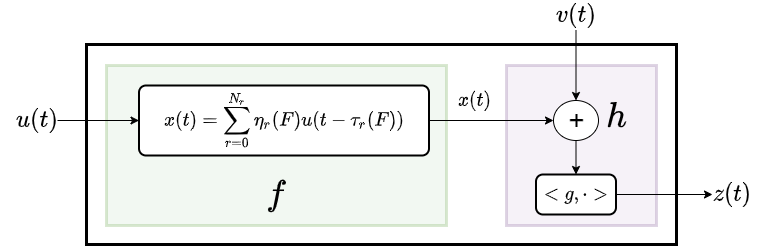
\includegraphics[width=0.9\textwidth]{./Radar-fixed_range}
        \caption{\label{fig:Radar-fixed_range}Block-diagram for true radar equations assuming a fixed range}
\end{figure}
%
\begin{figure}
    \centering
        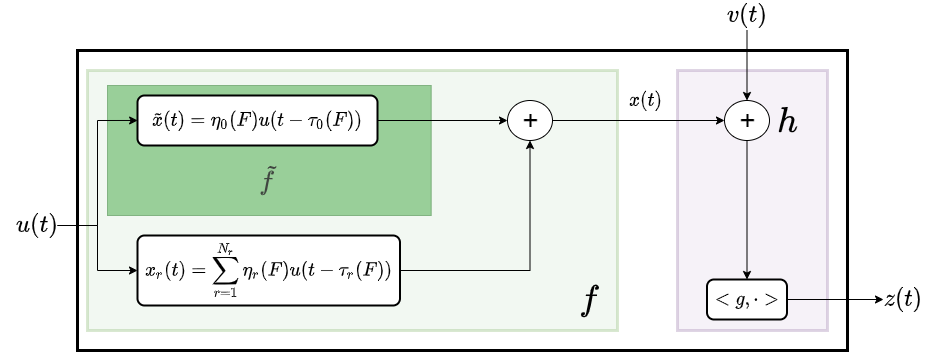
\includegraphics[width=0.9\textwidth]{./Radar-fixed_range_rearranged}
        \caption{\label{fig:Radar-fixed_range_rearranged}Rearranging the blocks in figure \ref{fig:Radar-fixed_range} and identifying the approximated system-model $\tilde{f}$}
\end{figure}
%
Re-arranging the elements in figure \ref{fig:Radar-fixed_range} we obtain figure \ref{fig:Radar-fixed_range_rearranged} in which we identify the approximated system-model $\tilde{f}$. The model of figure \ref{fig:Radar-fixed_range_rearranged} is a custom example for the general model depicted in figure \ref{fig:Radar-general} and in the following equations:
%
\begin{equation}\label{eq:generalResearchObjective}
    \begin{split}
        &\dot{\tilde{x}}(t) = \tilde{f}\left( u(t), \omega(t); F \right)\\
        %
        &x(t) = \tilde{x}(t) + f_r\left( u(t), \tilde{x}(t), \psi(t); F\right)\\
        %
        &z(t) = h\left( x(t), v(t)\right)
    \end{split}
\end{equation}
%
While the measurements are the outputs of the system described in equation \ref{eq:generalResearchObjective}, the estimator, either filtering or smoothing, performs estimations assuming $f_r\left( u(t), \tilde{x}(t), \psi(t); F\right) \equiv 0$. For a linear model in discrete-time equation \ref{eq:generalResearchObjective} becomes: 
%
\begin{equation}\label{eq:generalResearchObjective_lin}
    \begin{split}
        &\tilde{x}_{k+1} = F\tilde{x}_{k} + Gu_k +  \omega_k\\
        %
        &x^u_{k} = f_r\left( x^u_{k-1}, u_k, \tilde{x}_k, \psi_k; F\right)\\
        %
        &x_k = \tilde{x}_k + x^u_{k}\\
        %
        &z_k = H'x_k + v_k
    \end{split}
\end{equation}
%
The approximated model is obtained from equation \ref{eq:generalResearchObjective_lin} by setting $f_r ( \cdot ) \equiv 0$. If this was indeed the case then smoothing would have obtained smaller estimation errors. We would like to derive conditions on the unmodeled behaviour $f_r$ for which smoothing estimation errors are smaller than filtering estimation errors.\\\\

\textbf{Ronny} - given that $F$ and $G$ are known, estimations (assuming $f_r \equiv 0$) can be made using a standard Kalman filter. This case would be more straightforward to investigate. But, in the case of the physiological system as well as in the case of the radar, $F$ is unknown and is the objective of the estimation. What do you advise to investigate?  
%
%
\begin{figure}
    \centering
        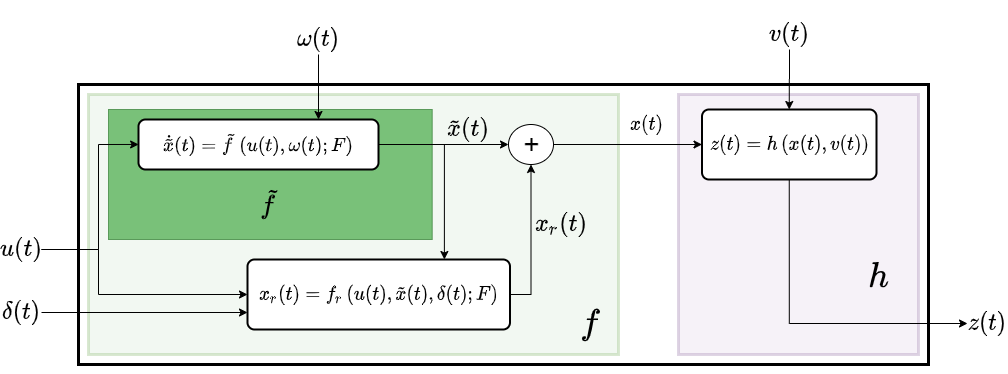
\includegraphics[width=0.9\textwidth]{./Radar-general}
        \caption{\label{fig:Radar-general}Proposed model for research}
\end{figure}
%
\section{Filtering vs. smoothing (approximated model) 30.06}\label{sec:F_vs_S}
%
In this section we derive the estimation error covariances for both filtering and smoothing in the presence of an unmodeled behaviour. We would like to obtain conditions on the unmodeled behaviour for which smoothing will have smaller estimation errors. We first manipulate equation \ref{eq:generalResearchObjective_lin} to present the unmodeled behaviour as a second sensor whose measurements are summed with the known sensor $h$. Substituting $x_k$ into $z_k$:
%
\begin{equation*}
    z_k = H'\tilde{x}_k + H'f_r\left( x^u_{k-1}, u_k, \tilde{x}_k, \psi_k; F\right) + v_k = H'\tilde{x}_k + v_k + s_k
\end{equation*}
%
with $s_k=H'f_r\left( x^u_{k-1}, u_k, \tilde{x}_k, \psi_k; F\right)$ is the measured unmodeled behaviour. Concluding, the true system is of the form
%
\begin{equation}\label{eq:generalResearchObjective_lin2}
    \begin{split}
        \tilde{x}_{k+1} &= F\tilde{x}_{k} + Gu_k +  \omega_k\\
        z_k &= H'\tilde{x}_k + v_k + s_k = \tilde{z}_k + s_k
    \end{split}
\end{equation}
%
with $\tilde{z}_k = H'\tilde{x}_k + v_k$ while the approximated system is obtained by setting $s_k \equiv 0$. \\($\tilde{x}_k,\omega_k$ are $n \times 1$; $z_k,v_k,s_k$ are $m \times 1$).\\\\
%
%
%
%\begin{figure}
%    \centering
%        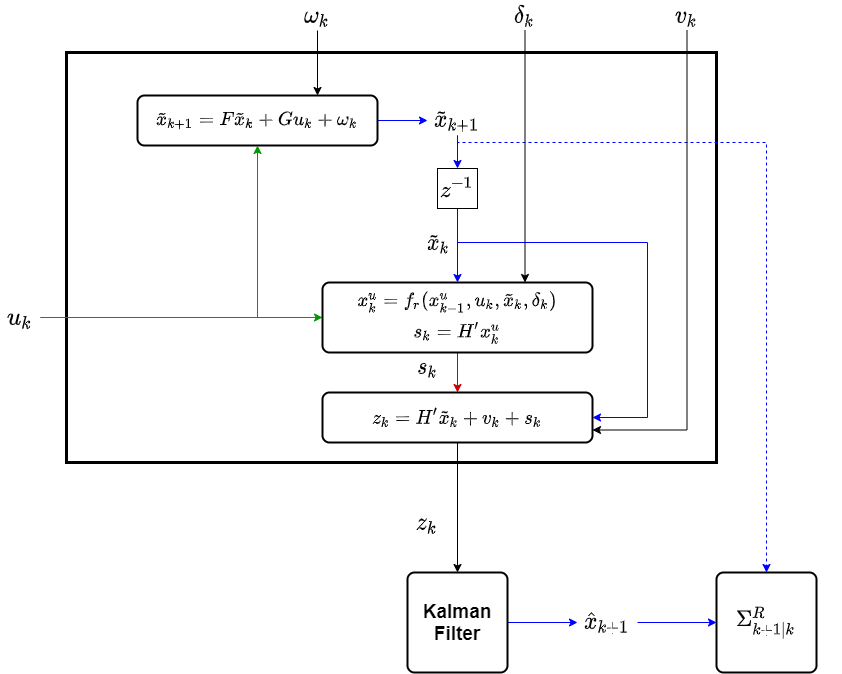
\includegraphics[width=0.8\textwidth]{./Radar-general_discrete}
%        \caption{\label{fig:Radar-general_discrete}System of equation \ref{eq:generalResearchObjective_lin2} and the Kalman filter}
%\end{figure}
%
The Kalman filter keeps an internal calculated error covariance $\Sigma_{k+1 \mid k}$ as well as a gain $K_k$. Both are independent of the received measurements $z_k$. We Assume that steady state values exists with $\operatorname{lim}_{k \xrightarrow{} \infty} \Sigma_{k \mid k-1}= \Bar{\Sigma}$ and $\operatorname{lim}_{k \xrightarrow{} \infty} K_k = K$ and are given in equations \ref{eq:sigma_bar} and \ref{eq:steadyGain}. Since the Kalman filter operates with respect to an approximated model the internal calculated error covariance $\Sigma_{k+1 \mid k}$ differs from the real error covariance which we denote by $\Sigma^R_{k+1 \mid k}$. \\\\
%
\begin{figure}
    \centering
        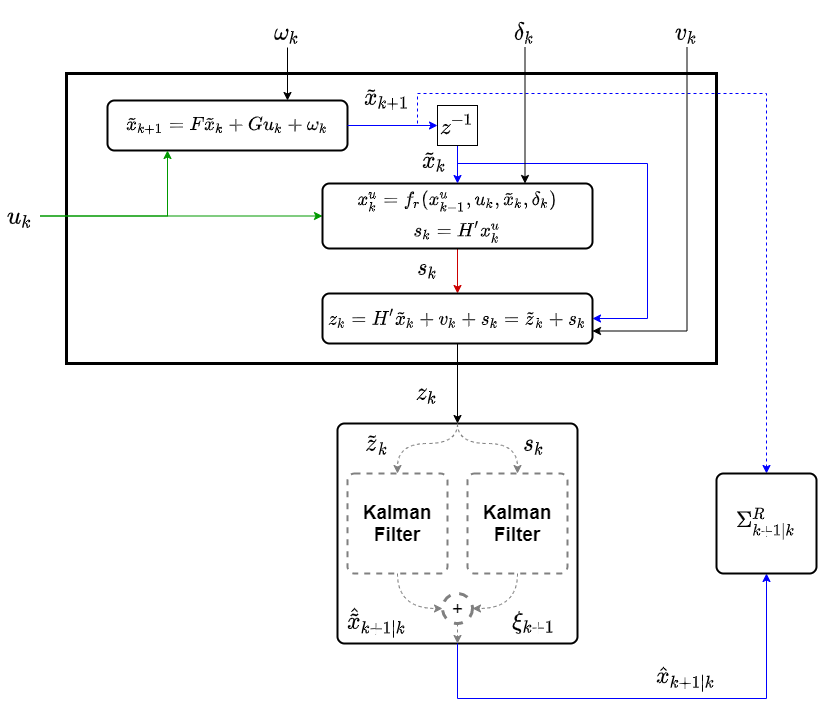
\includegraphics[width=0.8\textwidth]{./Radar-general-discrete02}
        \caption{\label{fig:Radar-general-discrete02}System of equation \ref{eq:generalResearchObjective_lin2} and an equivalent view of the Kalman filter by its linear properties. Note that the two Kalman filters in this figure are identical at all time instances}
\end{figure}
%
An elegant way to derive an expression relating $\Sigma^R_{k+1 \mid k}$ with the internal error covariance $\Sigma_{k+1 \mid k}$ calculated by the Kalman filter is by the linear property of the Kalman filter which is depicted in figure \ref{fig:Radar-general-discrete02} and yields: 
%
\begin{equation}\label{eq:errCov_linSplit}
    \begin{split}
        \Sigma^R_{k+1 \mid k} &= \operatorname{E}[(\tilde{x}_{k+1}-\hat{x}_{k+1 \mid k})(\tilde{x}_{k+1}-\hat{x}_{k+1 \mid k})']\\
        %
        &= \operatorname{E}[(\tilde{x}_{k+1}- \hat{\tilde{x}}_{k+1 \mid k} - \xi_{k+1})(\tilde{x}_{k+1}- \hat{\tilde{x}}_{k+1 \mid k} - \xi_{k+1})']\\
        %
        &= \operatorname{E}[(\tilde{x}_{k+1}- \hat{\tilde{x}}_{k+1 \mid k})(\tilde{x}_{k+1}- \hat{\tilde{x}}_{k+1 \mid k})']\\
        %
        &+ \left(\operatorname{E}[\xi_{k+1}\xi_{k+1}'] - \left( \operatorname{E}[\xi_{k+1}(\tilde{x}_{k+1}- \hat{\tilde{x}}_{k+1 \mid k})'] +  \operatorname{E}[(\tilde{x}_{k+1} - \hat{\tilde{x}}_{k+1 \mid k})\xi_{k+1}'] \right) \right)\\
        %
        &= \Sigma_{k+1 \mid k} + \left(\operatorname{E}[\xi_{k+1}\xi_{k+1}'] - \left( \operatorname{E}[\xi_{k+1}(\tilde{x}_{k+1}- \hat{\tilde{x}}_{k+1 \mid k})'] +  \operatorname{E}[(\tilde{x}_{k+1}- \hat{\tilde{x}}_{k+1 \mid k})\xi_{k+1}'] \right) \right)
    \end{split}
\end{equation}         
%
The fixed-point smoother (\href{https://technionmail-my.sharepoint.com/:b:/g/personal/ron_teichner_campus_technion_ac_il/EQjFqjBlxRxLsoQEzqjmZdAB2D_O3BBw_feZhde7ShqzAA?e=XATenX}{link to equations}) for estimating $\tilde{x}_j$ ($j$ is fixed) is a linear system. It is initialized at time $k=j$ with the current filtering-estimation of $x_j$ which is $\hat{x}_{j \mid j-1}$ and it operates for times $k \geq j$. Its input at time $k$ is the innovation process (with respect to the filter) $\bar{z}_k = z_k - H' \hat{x}_{k \mid k-1}$ and its output is $\hat{x}_{j \mid k}$ - the estimation of $x_j$ based on measurements up to and including time $k$. The input is a sum of a term given $s_k \equiv 0$ and a term due to the unmodeled behavior $s_k$:
%
\begin{equation}
    \begin{split}
        \bar{z}_k &= z_k - H' \hat{x}_{k \mid k-1}
        %
        = (\tilde{z}_k - H' \hat{\tilde{x}}_{k \mid k-1}) + (s_k - H'\xi_{k}) = \tilde{z}^s_k + s^s_k
    \end{split}
\end{equation}
%
where $\tilde{z}^s_k = \tilde{z}_k - H' \hat{\tilde{x}}_{k \mid k-1}$ is the input were there was no unmodeled bahvior present and $s^s_k = s_k - H'\xi_{k}$ is the additional term due to the unmodeled behaviour. Since the fixed-point smoother is a linear system it is equivalent to two identical smoothers operating on the two terms of the input as depicted in figure \ref{fig:Radar-general_discrete_03}. The output of the smoother, $\hat{x}_{j \mid k}$ is the sum of $\hat{\tilde{x}}_{j \mid k}$ which is the output of the smoother operating on $\tilde{z}_k^s$ and $\xi_k^s$ which is the output of the smoother operating on $s_k^s$.\\\\
%
\begin{figure}
    \centering
        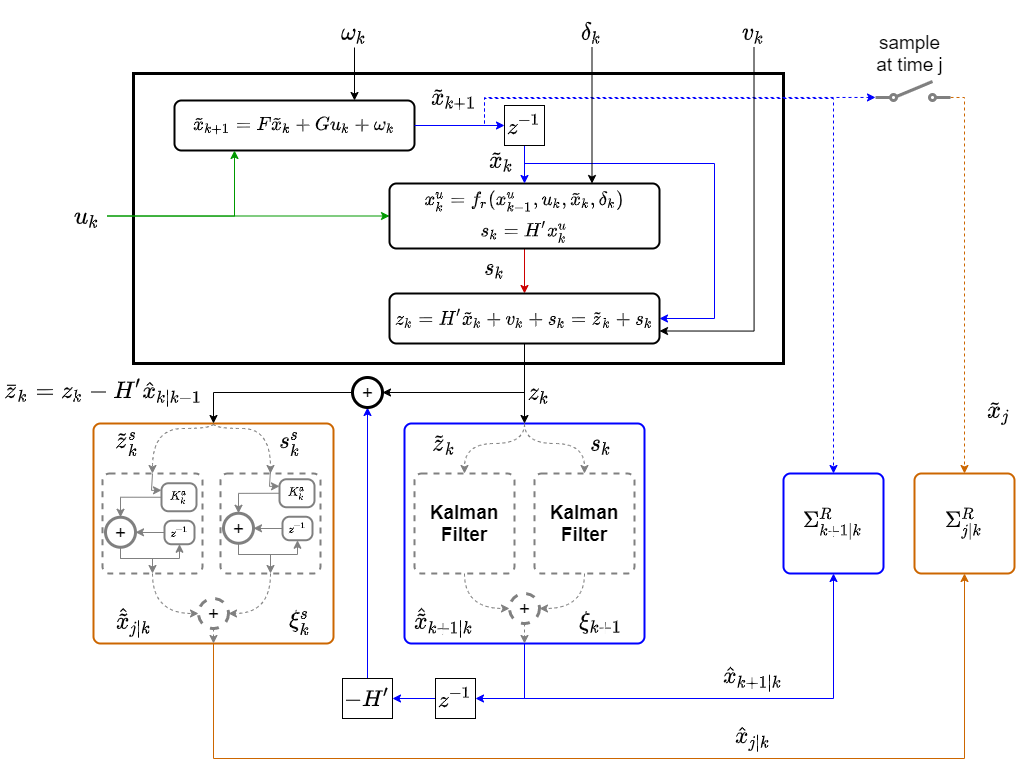
\includegraphics[width=0.8\textwidth]{./Radar-general_discrete_03}
        \caption{\label{fig:Radar-general_discrete_03}System of equation \ref{eq:generalResearchObjective_lin2} and an equivalent view of both the Kalman filter and fixed-point smoother by their linear properties. The smoother is initialized at time $k=j$ with the current filtering-estimation $\hat{x}_{j \mid j-1}$ and it operates for times $k \geq j$. The input to the smoother is $\bar{z}_k = z_k - H' \hat{x}_{k \mid k-1} = \tilde{z}^s_k + s^s_k$ with $\tilde{z}^s_k = \tilde{z}_k - H' \hat{\tilde{x}}_{k \mid k-1}$ and $s^s_k = s_k - H'\xi_{k}$.}
\end{figure}
%
The real smoothing error covariance, $\Sigma^R_{j \mid k}$ for $k \geq j$ can be related to $\Sigma_{j \mid k}$ which is the smoothing error covariance internally calculated by the smoother:
%
\begin{equation}\label{eq:smoothingErrCov_linSplit}
    \begin{split}
        \Sigma^R_{j \mid k} &= \operatorname{E}[(\tilde{x}_{j}-\hat{x}_{j \mid k})(\tilde{x}_{j}-\hat{x}_{j \mid k})']\\
        %
        &= \operatorname{E}[(\tilde{x}_{j} - \hat{\tilde{x}}_{j \mid k} - \xi_k^s)(\tilde{x}_{j} - \hat{\tilde{x}}_{j \mid k} - \xi_k^s)']\\
        %
        &= \operatorname{E}[(\tilde{x}_{j}- \hat{\tilde{x}}_{j \mid k})(\tilde{x}_{j}- \hat{\tilde{x}}_{j \mid k})']\\
        %
        &+ \left(\operatorname{E}[\xi^s_{k}\xi^s_{k}'] - \left( \operatorname{E}[\xi^s_{k}(\tilde{x}_{j}- \hat{\tilde{x}}_{j \mid k})'] +  \operatorname{E}[(\tilde{x}_{j} - \hat{\tilde{x}}_{j \mid k})\xi^s_{k}'] \right) \right)\\
        %
        &= \Sigma_{j \mid k} + \left(\operatorname{E}[\xi^s_{k}\xi^s_{k}'] - \left( \operatorname{E}[\xi^s_{k}(\tilde{x}_{j}- \hat{\tilde{x}}_{j \mid k})'] +  \operatorname{E}[(\tilde{x}_{j} - \hat{\tilde{x}}_{j \mid k})\xi^s_{k}'] \right) \right)
    \end{split}
\end{equation}         
%
For convenience we group together the real filtering and smoothing error covariances for the estimation of $\tilde{x}_j$ at times $k \geq j$:
%
\begin{equation}\label{eq:filteringSmoothingErrCovs}
    \begin{split}
        \Sigma^R_{j \mid j-1} &= \Sigma_{j \mid j-1} + \left(\operatorname{E}[\xi_{j}\xi_{j}'] - \left( \operatorname{E}[\xi_{j}(\tilde{x}_{j}- \hat{\tilde{x}}_{j \mid j-1})'] +  \operatorname{E}[(\tilde{x}_{j}- \hat{\tilde{x}}_{j \mid j-1})\xi_{j}'] \right) \right)\\
        %
        \Sigma^R_{j \mid k} &= \Sigma_{j \mid k} + \left(\operatorname{E}[\xi^s_{k}\xi^s_{k}'] - \left( \operatorname{E}[\xi^s_{k}(\tilde{x}_{j}- \hat{\tilde{x}}_{j \mid k})'] +  \operatorname{E}[(\tilde{x}_{j} - \hat{\tilde{x}}_{j \mid k})\xi^s_{k}'] \right) \right)
    \end{split}
\end{equation}  
%
There are known relations between $\Sigma_{j \mid j-1}$ and $\Sigma_{j \mid k}$ which are investigated thoroughly in Section \ref{sec:subKalman}. It is guaranteed that \Sigma_{j \mid k \geq j} \preceq $\Sigma_{j \mid j-1}$, which means that given $s_k \equiv 0$ smoothing results in smaller error covariance. Our goal is to find constrains on the unmodeled behaviour $s_k$ guaranteeing $\Sigma^R_{j \mid k} \preceq \Sigma^R_{j \mid j-1}$ for all $k \geq j$. Our strategy is to find constrains on $s_k$ guaranteeing that $\Sigma^R_{k \mid k} \preceq \Sigma^R_{k \mid k-1}$ meaning that the first future measurement always improves the estimation.\\\\
%
We claim that to guarantee that every obtained measurement improves the smoothing estimation, that is $\Sigma^R_{j \mid k} \preceq \Sigma^R_{j \mid j-1}$ for all $k \geq j$, it is enough to guarantee $\Sigma^R_{k \mid k} \preceq \Sigma^R_{k \mid k-1}$.\\
%
Proof:\\
%
Assume that $\Sigma^R_{k \mid k} \preceq \Sigma^R_{k \mid k-1}$ holds for all $k$ values and consider the estimation of the state at time $m-1$, $\tilde{x}_{m-1}$. By our assumption $\Sigma^R_{m-1 \mid m-1} \preceq \Sigma^R_{m-1 \mid m-2}$ and we will show that $\Sigma^R_{m-1 \mid m} \preceq \Sigma^R_{m-1 \mid m-1}$.\\
%
The estimation $\hat{\tilde{x}}_{m-1 \mid m-1}$ is based on the measurements $z_{1:m-1}$. This estimation is equivalent to an estimation of $\tilde{x}_{m-1}$ based on $\{z_{1:m-1},\hat{z}_{m \mid m-1}\}$ with $\hat{z}_{m \mid m-1} = H' F \hat{\tilde{x}}_{m-1 \mid m-1}$. The error associated with $\hat{z}_{m \mid m-1}$ is $\Sigma^R_{m \mid m-1}$.\\
%
Given the estimation $\hat{\tilde{x}}_{m \mid m}$ we can deduce $\hat{z}_{m \mid m} = H'F\hat{\tilde{x}}_{m \mid m}$ with its associated error $\Sigma^R_{m \mid m}$. According to our assumption, $\Sigma^R_{m \mid m} \preceq \Sigma^R_{m \mid m-1}$, therefore, $\hat{z}_{m \mid m}$ has a smaller associated error than $\hat{z}_{m \mid m-1}$.\\
%
As a result, estimating $\tilde{x}_{m-1}$ based on $\{z_{1:m-1},\hat{z}_{m \mid m}\}$ results in a smaller error covariance than estimating it based on $\{z_{1:m-1},\hat{z}_{m \mid m-1}\}$. We thus conclude that $\Sigma^R_{m-1 \mid m} \preceq \Sigma^R_{m-1 \mid m-1} \preceq \Sigma^R_{m-1 \mid m-2}$. Setting $j=m-1$ results in $\Sigma^R_{j \mid j+1} \preceq \Sigma^R_{j \mid j-1}$. It is straightforward to recursively obtain $\Sigma^R_{j \mid k} \preceq \Sigma^R_{j \mid j-1}$ for all $k \geq j$.   
%
%
%
\subsection{The unmodeled behaviour is white noise (05.07)}\label{sec:subWhiteNoise}
%
We start by assuming the unmodeled behavior is a white noise with a covariance matrix $Q^u$, independent of the assumed process and measurement noises:
%
\begin{equation}
    \begin{split}
        &s_k = H' \psi_k\\
        %
        &\operatorname{E}[\psi_k] = 0\\
        %
        &\operatorname{E}[\psi_k \psi_j'] = Q^u \delta(k-j)
    \end{split}
\end{equation}
%
We would like express equation \ref{eq:filteringSmoothingErrCovs} for this case. Due to the independence of all the noises we obtain for the filter:
%
\begin{equation}
    \operatorname{E}[\xi_{k}(\tilde{x}_{k}- \hat{\tilde{x}}_{k \mid k-1})'] = 0
\end{equation}
%
(full derivations at \href{https://technionmail-my.sharepoint.com/:b:/g/personal/ron_teichner_campus_technion_ac_il/EfuePiH-kmhMl9R80PHRhnMButsVxmWqnO2MVCnZFKkLaA?e=IvXfRv}{link1}, \href{https://technionmail-my.sharepoint.com/:b:/g/personal/ron_teichner_campus_technion_ac_il/EWJu12JzYTtOq0LrN7YbSkMB4ctEU_lpwbnc20nSpUXWPA?e=ELjyGu}{link2}). For the smoother:
%
\begin{equation}
    \begin{split}
        \operatorname{E}[\xi^s_{k}(\tilde{x}_{j}- \hat{\tilde{x}}_{j \mid k})'] &= \operatorname{E}[(\xi_j + \sum_{i=j}^{k} K^a_{i} s^s_{i})(\tilde{x}_{j}- \hat{\tilde{x}}_{j \mid k})']\\
        %
        &= \operatorname{E}[(\sum_{i=1}^{j} \tilde{F}^{i-1} K H' \psi_{j-i} + \sum_{i=j}^{k} K^a_{i} H'\psi_i)(\tilde{x}_{j}- \hat{\tilde{x}}_{j \mid k})']\\
        %
        &= \operatorname{E}[\sum_{i=0}^{j-1} \tilde{F}^{j-i-1} K H' \psi_{i} + \sum_{i=j}^{k} K^a_{i} H'\psi_i] \operatorname{E}[(\tilde{x}_{j}- \hat{\tilde{x}}_{j \mid k})'] = 0
    \end{split}
\end{equation}
%
%
Equation \ref{eq:filteringSmoothingErrCovs} therefore becomes:
%
\begin{equation}\label{eq:whiteNoiseCovs}
    \begin{split}
        \Sigma^R_{j \mid j-1} &= \Sigma_{j \mid j-1} + \operatorname{E}[\xi_{j}\xi_{j}']\\
        %
        \Sigma^R_{j \mid k} &= \Sigma_{j \mid k} + \operatorname{E}[\xi^s_{k}\xi^s_{k}']
    \end{split}
\end{equation}  
%
Substituting $\Sigma_{j \mid j-1} = \Bar{\Sigma}$ (the steady-state internal calculated filtering error covariance) and $\Sigma_{j \mid k}$ (the internal calculated smoothing error covariance) from equation \ref{eq:sigma_smoothing}:
%
\begin{equation}\label{eq:whiteNoiseCovs}
    \begin{split}
        &\Sigma^R_{j \mid j-1} = \Bar{\Sigma} + \operatorname{E}[\xi_{j}\xi_{j}']\\
        %
        &\Sigma^R_{j \mid k} = \Bar{\Sigma} - \Bar{\Sigma} \left[ \sum_{i=j}^k [\tilde{F}']^{i-j} H \left[ H' \Bar{\Sigma} H + R\right]^{-1}H'\tilde{F}^{i-j}\right]\Bar{\Sigma} + \operatorname{E}[\xi^s_{k}\xi^s_{k}']
    \end{split}
\end{equation}  
%
We can now evaluate the difference between filtering and smoothing error covariances in the presence of the unmodeled behavior, $\Sigma^R_{j \mid j-1} - \Sigma^R_{j \mid k}$:
%
\begin{equation}\label{eq:realFilteringVsSmoothing}
    \begin{split}
        \Delta^R_{j,k} = \Sigma^R_{j \mid j-1} - \Sigma^R_{j \mid k} = 
        \Bar{\Sigma} \left[ \sum_{i=j}^k [\tilde{F}']^{i-j} H \left[ H' \Bar{\Sigma} H + R\right]^{-1}H'\tilde{F}^{i-j}\right]\Bar{\Sigma} 
        + \operatorname{E}[\xi_{j}\xi_{j}'] - \operatorname{E}[\xi^s_{k}\xi^s_{k}']
    \end{split}
\end{equation}
%
%
To proceed we will derive an expression for $\operatorname{E}[\xi^s_{k}\xi^s_{k}']$.
%
\subsection*{Derivation of $\operatorname{E}[\xi^s_{k}\xi^s_{k}']$}
%
Let us begin by analyzing the process $\xi_k$. The output of the (imaginary) Kalman-filter whose input is $s_k$ and its initialization value is $0$ is given by equation \ref{eq:kalmanGeneralExp}:
%
\begin{equation}
    \begin{split}
        \xi_{k+1} &= \sum_{i=1}^{k+1} \tilde{F}^{i-1} K s_{k+1-i}
    \end{split}
\end{equation}
%
substituting $s_{k} = H' \psi_{k}$:
%
\begin{equation}\label{eq:kalmanUnmodeledOutput}
    \begin{split}
        \xi_{k} &= \sum_{i=1}^{k} \tilde{F}^{i-1} K H' \psi_{k-i} = \tilde{F}\xi_{k-1} + KH' \psi_{k-1}
    \end{split}
\end{equation}
%
with $\tilde{F} = F - K H'$ as given in equation \ref{eq:steadyGain}. The mean of the process $\xi_k$ is constant for all times:
%
\begin{equation}\label{eq:filterOutMean}
    \begin{split}
        &\operatorname{E}[\xi_k] = \operatorname{E}[\sum_{i=1}^{k} \tilde{F}^{i-1} K H' \psi_{k-i}] = \sum_{i=1}^{k} \tilde{F}^{i-1} K H' \operatorname{E}[ \psi_{k-i}] = 0
    \end{split}
\end{equation}        
%
and its autocovariance $R_{\xi}(k,m) = \operatorname{E}[\xi_k \xi_m']$ is:
%
\begin{equation}\label{eq:filterOutAutoCovNotethat}
    \begin{split}
        R_{\xi}(k,k) &= \sum_{i=1}^{k} \tilde{F}^{i-1} K H' Q^u H K' \tilde{F}^{i-1}'\\
        %
        R_{\xi}(k,m \geq k) &= R_{\xi}(k,k) \tilde{F}^{m-k}'\\
        %
        R_{\xi}(k,m<k) &= \tilde{F}^{k-m} R_{\xi}(m,m)\\
    \end{split}
\end{equation}
%
for the complete derivation see equations \ref{eq:filterOutAutoCov_comp}, \ref{eq:filterOutAutoCovNotethat_comp}.\\\\
%
The mean of the process $s^s_k$, the input to the (imaginary) smoother, is constant for all times:
%
\begin{equation}\label{eq:smoothInMean}
    \begin{split}
        \operatorname{E}[s^s_k] = \operatorname{E}[s_k - H'\xi_k] = \operatorname{E}[s_k] - H'\operatorname{E}[\xi_k] = H'\operatorname{E}[\psi_k] - H'\operatorname{E}[\xi_k] = 0
    \end{split}
\end{equation}
%
Its autocovariance $R_{s^s}(k,m) = \operatorname{E}[s^s_k s^s_m]$ is:
%
\begin{equation}\label{eq:smootherInAutoCovNoteThat}
    \begin{split}
        R_{s^s}(k,k) &= H' Q^u H + H' R_{\xi}(k,k) H\\ 
        R_{s^s}(k,m < k) &=- H' \tilde{F}^{k-m-1} K H' Q^u H + H' \tilde{F}^{k-m} R_{\xi}(m,m) H\\ 
        %
        R_{s^s}(k,m>k) &=- H' Q^u  H K' \tilde{F}^{m-k-1}'H + H' R_{\xi}(k,k) \tilde{F}^{m-k}' H\\ 
    \end{split}
\end{equation}
%
for the complete derivation see equations \ref{eq:smootherInAutoCov_comp}, \ref{eq:smootherInAutoCovNoteThat_comp}.\\\\
%
Finally we consider the process $\xi^s_k$ at the output of the (imaginary) smoother. The initialization value of the smoother is the filtering-estimation for $\tilde{x}_j$ which is:
%
\begin{equation}\label{eq:smootherInit}
    \hat{x}_{j \mid j-1} = \hat{\tilde{x}}_{j \mid j-1} + \xi_j
\end{equation}
%
For the (imaginary) smoother whose input is $s^s_k$ and initialization value is $\xi_j$, from equation \ref{eq:smootherGeneral} we obtain:
%
\begin{equation}
    \xi_k^s = \xi_j + \sum_{i=j}^{k} K^a_{i} s^s_{i}
\end{equation}
The mean of $\xi^s_k$ (based on equations \ref{eq:filterOutMean}, \ref{eq:smoothInMean}) is:
%
\begin{equation}
    \begin{split}
        \operatorname{E}[\xi^s_k] = \operatorname{E}[\xi_j + \sum_{i=j}^{k} K^a_{i} s^s_{i}] = \operatorname{E}[\xi_j] + \sum_{i=j}^{k} K^a_{i} \operatorname{E}[ s^s_{i}] = 0
    \end{split}
\end{equation}
%
The autocovariance of $\xi^s_k$ is:
%
\begin{equation}
    \begin{split}
        &R_{\xi^s}(k,m) = \operatorname{E}[(\xi^s_k - \operatorname{E}[\xi^s_k]) (\xi^s_m - \operatorname{E}[\xi^s_m])'] = \operatorname{E}[\xi^s_k \xi^s_m'] = \operatorname{E}[(\xi_j + \sum_{i=j}^{k} K^a_{i} s^s_{i}) (\xi_j + \sum_{i=j}^{m} K^a_{i} s^s_{i})']
    \end{split}
\end{equation}
%
%
%
and for $k \geq j$:
\begin{equation}\label{eq:smootherEnergy}
    \begin{split}
        R_{\xi^s}(k,k) = \operatorname{E}[\xi^s_{k}\xi^s_{k}'] &= \operatorname{E}[(\xi_j + \sum_{i=j}^{k} K^a_{i} s^s_{i})(\xi_j + \sum_{i=j}^{k} K^a_{i} s^s_{i})']\\
        %
        &= \operatorname{E}[\xi_j \xi_j'] + \operatorname{E}[\xi_j \sum_{i=j}^{k} s^s_{i}' K^a_{i}'] + \operatorname{E}[\sum_{i=j}^{k} K^a_{i} s^s_{i} \xi_j'] + \operatorname{E}[(\sum_{i=j}^{k} K^a_{i} s^s_{i}) (\sum_{m=j}^{k} s^s_{m}' K^a_{m}' )]\\
        %
        &= \operatorname{E}[\xi_j \xi_j'] + 
        \sum_{i=j}^{k} \operatorname{E}[  \xi_j s^s_{i}' ] K^a_{i}' + \sum_{i=j}^{k} K^a_{i} \operatorname{E}[  s^s_{i} \xi_j'] + \sum_{i=j}^{k} \sum_{m=j}^{k} K^a_{i} \operatorname{E}[ s^s_{i}  s^s_{m}' ] K^a_{m}'
    \end{split}
\end{equation}
%
Evaluation of $\operatorname{E}[  \xi_j s^s_{i \geq j}' ]$, $\operatorname{E}[  s^s_{i \geq j} \xi_j']$:
%
\begin{equation}
    \begin{split}
        \operatorname{E}[  \xi_j s^s_{i \geq j}' ] &= \operatorname{E}[  \xi_j (s_{i \geq j} - H' \xi_{i \geq j})' ] = \operatorname{E}[  \xi_j s_{i \geq j}'] - \operatorname{E}[  \xi_j \xi_{i \geq j}' ] H = -R_{\xi}(j,i) H\\
        %
        \operatorname{E}[  s^s_{i \geq j} \xi_j'] &= \operatorname{E}[  (s_{i \geq j} - H' \xi_{i \geq j}) \xi_j'] 
        = \operatorname{E}[  s_{i \geq j}  \xi_j'] - H' \operatorname{E}[ \xi_{i \geq j} \xi_j'] = -H' R_{\xi}(i,j)
    \end{split}
\end{equation}
%
since the output $\xi_j$ at time $j$ is independent of future input measurements $s_{i \geq j}$. Substituting into equation \ref{eq:smootherEnergy} we obtain:
%
\begin{equation}\label{eq:smootherUnmodeledAutoCov}
    \begin{split}
        \operatorname{E}[\xi^s_{k}\xi^s_{k}'] &= \operatorname{E}[\xi_j \xi_j'] - (\sum_{i=j}^{k} R_{\xi}(j,i) H K^a_{i}' + \sum_{i=j}^{k} K^a_{i} H' R_{\xi}(i,j)  - \sum_{i=j}^{k} \sum_{m=j}^{k} K^a_{i} R_{s^s}(i,m) K^a_{m}')
    \end{split}
\end{equation}
%
which completes our derivation of $\operatorname{E}[\xi^s_{k}\xi^s_{k}']$.
%
\subsection*{Analyzing $\Delta^R_{j,k} = \Sigma^R_{j \mid j-1} - \Sigma^R_{j \mid k}$}
%
%
%
Substituting the result obtained for $\operatorname{E}[\xi^s_{k}\xi^s_{k}']$ (equation \ref{eq:smootherUnmodeledAutoCov}) into equation \ref{eq:realFilteringVsSmoothing}:
%
\begin{equation}\label{eq:realFilteringVsSmoothing02}
    \begin{split}
        \Delta^R_{j,k} &= \Sigma^R_{j \mid j-1} - \Sigma^R_{j \mid k}\\
        %
        &= \Bar{\Sigma} \left[ \sum_{i=j}^k [\tilde{F}']^{i-j} H \left[ H' \Bar{\Sigma} H 
        + R\right]^{-1}H'\tilde{F}^{i-j}\right]\Bar{\Sigma} 
        +\sum_{i=j}^{k} R_{\xi}(j,j) \tilde{F}^{i-j}' H K^a_{i}'
        + \sum_{i=j}^{k} K^a_{i} H' \tilde{F}^{i-j} R_{\xi}(j,j)
        \\
        %
        &  - \sum_{i=j}^{k} \sum_{m=j}^{k} K^a_{i} R_{s^s}(i,m) K^a_{m}'
    \end{split}
\end{equation}
%
full derivation at equation \ref{eq:realFilteringVsSmoothing02_comp}.\\\\
%
We would like to obtain constrains on $Q^u$ under which $\Delta^R_{j,k} \succeq 0$ for all $k \geq j$. As shown, it is enough to obtain constrains under which a single sample from the future improves the estimation error, $\Delta^R_{j,j} \succeq 0$. Taking equation \ref{eq:realFilteringVsSmoothing02} with $k=j$:
%
\begin{equation}\label{eq:realFilteringVsSmoothingSingleSample}
    \begin{split}
        \Delta^R_{j,j} = \Sigma^R_{j \mid j-1} - \Sigma^R_{j \mid j} &= \Bar{\Sigma}   H \left[ H' \Bar{\Sigma} H + R\right]^{-1}H'\Bar{\Sigma} + (R_{\xi}(j,j) H K^a_{j}' + K^a_{j} H' R_{\xi}(j,j)  -  K^a_{j} R_{s^s}(j,j) K^a_{j}')\\
    \end{split}
\end{equation}
%
From equations \ref{eq:filterOutAutoCovNotethat} and \ref{eq:smootherInAutoCovNoteThat} we have that:
%
\begin{equation}\label{eq:R_xi_j_j}
    \begin{split}
         R_{\xi}(j,j) &= \sum_{i=0}^{j-1} \tilde{F}^{i} K H' Q^u H K' \tilde{F}^{i}'\\% \preceq \bar{R_{\xi}}\\
         %
         R_{s^s}(j,j) &= H' Q^u H + H' R_{\xi}(j,j) H% \preceq H' Q^u H + H' \bar{R_{\xi}} H \\ 
    \end{split}
\end{equation}
%
%with $\bar{R_{\xi}} = \sum_{i=0}^{\infty} \tilde{F}^{i} K H' Q^u H K' \tilde{F}^{i}'$ which exists by Lemma 2.1 @ Anderson&Moore and is positive definite. 
substituting $R_{s^s}(j,j)$ into equation \ref{eq:realFilteringVsSmoothingSingleSample}:
%
\begin{equation}\label{eq:realFilteringVsSmoothingSingleSample01}
    \begin{split}
        \Delta^R_{j,j} &= \Bar{\Sigma}   H \left[ H' \Bar{\Sigma} H + R\right]^{-1}H'\Bar{\Sigma} + (R_{\xi}(j,j) H K^a_{j}' + K^a_{j} H' R_{\xi}(j,j)  -   K^a_{j} H' Q^u H K^a_{j}' - K^a_{j} H' R_{\xi}(j,j) H K^a_{j}') 
    \end{split}
\end{equation}
%
From equation \ref{eq:smootherGain} we have that the gain of the smoother for the first future measurement is:
%
%
\begin{equation}
    \begin{split}
        &K^a_j = \Bar{\Sigma} [F \Bar{\Sigma}]^{-1} K
    \end{split}
\end{equation}
% K^a_j' = K' [F \Bar{\Sigma}]^{-1}' \Bar{\Sigma} 
For $j \gg 1$ we define $R_\xi(j,j) \approx \Bar{R_\xi}$ ($\Bar{R_\xi}$ exists according to Anderson). Substituting $K^a_j$, $\Bar{R_\xi}$ into equation \ref{eq:realFilteringVsSmoothingSingleSample01} and applying the desired inequality $\Delta^R_{j,j} \succeq 0$:
%
%
%
\begin{equation}\label{eq:SingleSampleWhiteNoiseFinalInequality}
    \begin{split}
        &\Bar{\Sigma}   H \left[ H' \Bar{\Sigma} H + R\right]^{-1}H'\Bar{\Sigma}\\ 
        %
        &+ (\Bar{R_\xi} H K' F^{-1}' + F^{-1} K H' \Bar{R_\xi}  -   F^{-1} K H' Q^u H K' F^{-1}' - F^{-1} K H' \Bar{R_\xi} H K' F^{-1}') \succeq 0
    \end{split}
\end{equation}
%
Since $\Bar{R_\xi}$ is a function of $Q^u$ we successfully derived an analytic (yet implicit) inequality from which $Q^u$ values guaranteeing that the first sample processed by the smoother improves the estimation error are obtained. As mentioned this guarantees that all samples processed by the smoother improve the estimation.\\\\
%
Trying to simplify the expression (and removing the constrain of $F^{-1}$). We again substitute into equation \ref{eq:realFilteringVsSmoothingSingleSample01} and apply the desired inequality $\Delta^R_{j,j} \succeq 0$:
%
%
\begin{equation}
    \begin{split}
        &\Bar{\Sigma} 
        \left(H \left[ H' \Bar{\Sigma} H + R\right]^{-1}H'
        - [F \Bar{\Sigma}]^{-1} K H' (Q^u + \Bar{R_\xi}) H K' [F \Bar{\Sigma}]^{-1}' \right)\Bar{\Sigma}\\
        &+ \Bar{R_\xi} H K' [F \Bar{\Sigma}]^{-1}' \Bar{\Sigma} 
        + \Bar{\Sigma} [F \Bar{\Sigma}]^{-1} K H' \Bar{R_\xi}  
          \succeq 0
    \end{split}
\end{equation}
%
Now, if it happens that
\begin{equation}
    \Bar{R_\xi} H K' [F \Bar{\Sigma}]^{-1}' \Bar{\Sigma} 
        + \Bar{\Sigma} [F \Bar{\Sigma}]^{-1} K H' \Bar{R_\xi}  
          \succeq 0
\end{equation}
%
then a sub-optimal constrain can be derived from
%
\begin{equation}
    \Bar{\Sigma} 
         \left(H \left[ H' \Bar{\Sigma} H + R\right]^{-1}H'
        - [F \Bar{\Sigma}]^{-1} K H' (Q^u + \Bar{R_\xi}) H K' [F \Bar{\Sigma}]^{-1}' \right)\Bar{\Sigma} \succeq 0
\end{equation}
%
which is equivalent to 
%
%
\begin{equation}
        H \left[ H' \Bar{\Sigma} H + R\right]^{-1}H'
        - [F \Bar{\Sigma}]^{-1} K H' (Q^u + \Bar{R_\xi}) H K' [F \Bar{\Sigma}]^{-1}' \succeq 0
\end{equation}
%
and results in:
%
\begin{equation}\label{eq:subOptimalConstrain}
        Q^u + \Bar{R_\xi} \preceq ([F \Bar{\Sigma}]^{-1} K H')^{-1} H \left[ H' \Bar{\Sigma} H + R\right]^{-1}H' (H K' [F \Bar{\Sigma}]^{-1}')^{-1}
\end{equation}
%
It is reasonable to assume that in the extreme case in which the 'unmodeled behavior player' has no information regarding the dynamic system we have that $Q^u = \sigma_u^2 I$. For this case we obtain an explicit bound on $\sigma_u^2$. First, $R_{\xi}(j,j)$ in equation \ref{eq:R_xi_j_j} becomes:
%
%
\begin{equation}\label{eq:R_xi_j_j}
    \begin{split}
         R_{\xi}(j,j) &= \sigma_u^2 \sum_{i=0}^{j-1} \tilde{F}^{i} K H' H K' \tilde{F}^{i}'
    \end{split}
\end{equation}
%
Then, for $j \gg 1$ we define $R_\xi(j,j) \approx \sigma_u^2 \tilde{R_\xi}$ and again substitute into equation \ref{eq:realFilteringVsSmoothingSingleSample01}:
%
%
\begin{equation}\label{eq:verySimpleBound}
    \begin{split}
          &B^{-1}C  \preceq \frac{1}{\sigma_u^2} I
    \end{split}
\end{equation}
%
with
%
\begin{equation}
    \begin{split}
          A &= \left[ H' \Bar{\Sigma} H + R\right]^{-1}H'\Bar{\Sigma}\\
          %
          B &= \Bar{\Sigma} H A\\
          %
          C &= \tilde{R_\xi} H A + A' H' \tilde{R_\xi} - A'H'(I+\tilde{R_\xi})H A
    \end{split}
\end{equation}
%
full derivation at equations \ref{eq:verySimpleBound_comp01} - \ref{eq:verySimpleBound_comp03}.
%
\subsubsection*{1-D case analysis}
%
Let us inspect the 1-D case for which we can obtain an explicit constrain on $Q^u$.
%
\begin{equation}
    \begin{split}
         R_{\xi}(j,j) &= \sum_{i=1}^{j} \tilde{F}^{i-1} K H' Q^u H K' \tilde{F}^{i-1}'= K^2 H^2 Q^u \tilde{F}^{-2} \sum_{i=1}^{j} \tilde{F}^{2i} 
         = K^2 H^2 Q^u  \frac{1-\tilde{F}^j}{1-\tilde{F}^2}
    \end{split}
\end{equation}
%
For $j \gg 1$, and since $|\tilde{F}|<1$ we have that
%
\begin{equation}
    \begin{split}
         R_{\xi}(j,j) \approx \Bar{R_\xi} = K^2 H^2 Q^u  \frac{1}{1-\tilde{F}^2}
    \end{split}
\end{equation}
%
%
substituting into inequality \ref{eq:SingleSampleWhiteNoiseFinalInequality} and using equation \ref{eq:steadyGain} for the steady-state filtering gain $K$ we derive a constrain on $Q^u$:
%
%
\begin{equation}\label{eq:realFilteringVsSmoothingSingleSample02}
    \begin{split}
        \Delta^R_{j,j} = \Sigma^R_{j \mid j-1} - \Sigma^R_{j \mid j} &= \Bar{\Sigma}^2   H^2 \left[ H' \Bar{\Sigma} H + R\right]^{-1} + \frac{Q^u H^2 K^2 }{F^2(1-\tilde{F}^2)}(  F^2 - 1) > 0\\
        %
        Q^u &< \frac{F^2(1-\tilde{F}^2) \Bar{\Sigma}^2}{ K^2(\Bar{\Sigma} H^2 + R)(1-F^2)}\\ 
        %
        &= \frac{F^2(1-\tilde{F}^2) \Bar{\Sigma}^2}{ (F \Bar{\Sigma}H(H'\Bar{\Sigma}H+R)^{-1})^2(\Bar{\Sigma} H^2 + R)(1-F^2)}\\
        %
        &= \frac{(1-\tilde{F}^2) (\Bar{\Sigma} H^2 + R)}{ H^2(1-F^2)}\\
        %
        &= \frac{(1-(F - KH)^2) (\Bar{\Sigma} H^2 + R)}{ H^2(1-F^2)}\\
        %
        &= \frac{(1-(F - \frac{F \Bar{\Sigma}H}{H^2 \Bar{\Sigma} + R}H)^2) (\Bar{\Sigma} H^2 + R)}{ H^2(1-F^2)}\\
    \end{split}
\end{equation}
%
%
It is easy to see that $\frac{(1-\tilde{F}^2) (\Bar{\Sigma} H^2 + R)}{ H^2(1-F^2)} > 0$ so that $Q^u$ is upper bounded by a positive number.\\\\
%
For the 1-D case, we explicitly derived a constrain on $Q^u$ that depends on the parameters of the modeled system. The constrain guarantees that the first sample and thus all samples processed by the smoother improve the estimation.\\\\
%
Evaluating the sub-optimal constrain from equation \ref{eq:subOptimalConstrain} for the 1-D case:
%
\begin{equation}
        Q^u  < \frac{(1-\tilde{F}^2) (\Bar{\Sigma} H^2  + R) }
        {H^2(1-F^2 + 2FKH  )}
\end{equation}
%
Indeed it is sub-optimal because:
%
%
\begin{equation}
        Q^u  < \frac{(1-\tilde{F}^2) (\Bar{\Sigma} H^2  + R) }
        {H^2(1-F^2 + 2FKH  )} < \frac{(1-\tilde{F}^2) (\Bar{\Sigma} H^2  + R) }
        {H^2(1-F^2)}
\end{equation}
%
This bound is relevant only if $1-F^2 + 2FKH > 0$:
%
\begin{equation}
    \begin{split}
        1-F^2 + 2FKH = 1 - F(F - 2KH) = 1 - F(\tilde{F} - KH) = 1 - F\tilde{F} + FKH >  1 - F\tilde{F} > 0
    \end{split}
\end{equation}
%
Assuming all numbers here are positive (which I believe is the case). 
%
%
\section{Appendix}\label{sec:appendix}
Derivation of eq. \ref{eq:sigma_bar}:
%
\begin{equation*}
    \begin{split}
        \Bar{\sigma}_e^2 &= f \left[\Bar{\sigma}_e^2 - \Bar{\sigma}_e^2 h \left( h\Bar{\sigma}_e^2 h+\sigma_v^2 \right)^{-1}h'\Bar{\sigma}_e^2 \right] f + \sigma_w^2\\
        %
        \Bar{\sigma}_e^2 &= f^2\Bar{\sigma}_e^2 - f^2 h^2 \left( h\Bar{\sigma}_e^2 h+\sigma_v^2 \right)^{-1}\Bar{\sigma}_e^4 + \sigma_w^2\\
        %
        \Bar{\sigma}_e^2 &= f^2\Bar{\sigma}_e^2 - \frac{f^2 h^2 \Bar{\sigma}_e^4}{h\Bar{\sigma}_e^2 h+\sigma_v^2} + \sigma_w^2\\
        %
        (h\Bar{\sigma}_e^2 h+\sigma_v^2)\Bar{\sigma}_e^2 &= (h\Bar{\sigma}_e^2 h+\sigma_v^2)f^2\Bar{\sigma}_e^2 - f^2 h^2 \Bar{\sigma}_e^4 + (h\Bar{\sigma}_e^2 h+\sigma_v^2)\sigma_w^2\\
        %
        h^2\Bar{\sigma}_e^4 + \sigma_v^2\Bar{\sigma}_e^2 &= h^2 f^2\Bar{\sigma}_e^4 + \sigma_v^2f^2\Bar{\sigma}_e^2 - f^2 h^2 \Bar{\sigma}_e^4 + h^2\sigma_w^2\Bar{\sigma}_e^2 + \sigma_v^2\sigma_w^2\\
        %
        0&= h^2\Bar{\sigma}_e^4 + (\sigma_v^2-\sigma_v^2f^2-h^2\sigma_w^2)\Bar{\sigma}_e^2 -\sigma_v^2\sigma_w^2\\
        %
        \Bar{\sigma}_e^2 &= \frac{-(\sigma_v^2-\sigma_v^2f^2-h^2\sigma_w^2) \pm \sqrt{(\sigma_v^2-\sigma_v^2f^2-h^2\sigma_w^2)^2 + 4h^2\sigma_v^2\sigma_w^2}}{2h^2}\\
        %
        \Bar{\sigma}_e^2 &= \frac{\sigma_v^2(f^2-1)+h^2\sigma_w^2 \pm \sqrt{(f^2-1)^2\sigma_v^4 + 2h^2\sigma_\omega^2(f^2+1)\sigma_v^2+(h^2\sigma_\omega^2)^2}}{2h^2}\\
        %
        \Bar{\sigma}_e^2 &= \frac{\sigma_v^2(f^2-1)+h^2\sigma_w^2 + \sqrt{(\sigma_v^2(f^2-1)+h^2\sigma_w^2)^2 + (2h\sigma_\omega\sigma_v)^2}}{2h^2}\\
    \end{split}
\end{equation*}
%
Lines of equal $\Bar{\sigma}_e^2$ are:  
%
\begin{equation*}
    \begin{split}
        \Bar{\sigma}_e^2 - 0.5(\sigma_v^2(f^2-1) + \sigma_w^2) &= 0.5\sqrt{(\sigma_v^2(f^2-1) + \sigma_w^2)^2 + (2\sigma_\omega\sigma_v)^2}\\
        %
        (\Bar{\sigma}_e^2 - 0.5(\sigma_v^2(f^2-1) + \sigma_w^2))^2 &= 0.25\left((\sigma_v^2(f^2-1) + \sigma_w^2)^2 + (2\sigma_\omega\sigma_v)^2\right)\\
        %
        \Bar{\sigma}_e^4 - \Bar{\sigma}_e^2(\sigma_v^2(f^2-1) + \sigma_w^2) + 0.25(\sigma_v^2(f^2-1) + \sigma_w^2)^2 &= 0.25(\sigma_v^2(f^2-1) + \sigma_w^2)^2 + 0.25(2\sigma_\omega\sigma_v)^2\\
        %
        \Bar{\sigma}_e^4 - \Bar{\sigma}_e^2(\sigma_v^2(f^2-1) + \sigma_w^2) &= 0.25(2\sigma_\omega\sigma_v)^2\\
        %
        \Bar{\sigma}_e^4 - \Bar{\sigma}_e^2\sigma_v^2(f^2-1) - \Bar{\sigma}_e^2\sigma_w^2 &= \sigma_\omega^2\sigma_v^2\\
        %
        \sigma_v^2(- \Bar{\sigma}_e^2(f^2-1) - \sigma_\omega^2) &= \Bar{\sigma}_e^2\sigma_w^2 - \Bar{\sigma}_e^4\\
        %
        \sigma_v^2 &= \Bar{\sigma}_e^2 \frac{\Bar{\sigma}_e^2 - \sigma_w^2}{\Bar{\sigma}_e^2(f^2-1) + \sigma_\omega^2}
    \end{split}
\end{equation*}
%
We must have $\sigma_v^2 > 0$.
%
\\If $\Bar{\sigma}_e^2 > \sigma_\omega^2$ then $\Bar{\sigma}_e^2(f^2-1) + \sigma_\omega^2 > 0 \xrightarrow{\abs{f} < 1} \Bar{\sigma}_e^2 < \frac{\sigma_\omega^2}{1-f^2}$ thus we have $1 < \frac{\Bar{\sigma}_e^2}{\sigma_\omega^2} < \frac{1}{1-f^2}$. 
%
\\If $\Bar{\sigma}_e^2 < \sigma_\omega^2$ then $\Bar{\sigma}_e^2(f^2-1) + \sigma_\omega^2 < 0 \xrightarrow{\abs{f} < 1} \Bar{\sigma}_e^2 > \frac{\sigma_\omega^2}{1-f^2}$ thus we have $\frac{1}{1-f^2} < \frac{\Bar{\sigma}_e^2}{\sigma_\omega^2} < 1$ which is not possible since $\frac{1}{1-f^2} > 1$.\\\\
%
Derivation of eq. \ref{eq:lin_f_1}:
%
\begin{equation}
    \begin{split}
        \frac{\Bar{\sigma}_e^2 + \sigma_v^2}{\Bar{\sigma}_e^2 + 2\sigma_v^2} &= c'\\
        %
        \Bar{\sigma}_e^2 &= \sigma_v^2\frac{2c'-1}{1-c'}\\
        %
        \Bar{\sigma}_e^2 &= 0.5\sigma_w^2 + 0.5\sqrt{\sigma_w^2(\sigma_w^2 + 4\sigma_v^2)}\\
        %
        0.5\sigma_w^2 + 0.5\sqrt{\sigma_w^2(\sigma_w^2 + 4\sigma_v^2)} &= \sigma_v^2\frac{2c'-1}{1-c'} = \sigma_v^2 c''\\
        %
        0.5\sqrt{\sigma_w^2(\sigma_w^2 + 4\sigma_v^2)} &= \sigma_v^2c'' - 0.5\sigma_w^2\\
        %
        0.25(\sigma_w^2(\sigma_w^2 + 4\sigma_v^2)) &= (\sigma_v^2c'' - 0.5\sigma_w^2)^2\\
        %
        0.25\sigma_w^4 + \sigma_w^2\sigma_v^2 &= {c''}^2\sigma_v^4 - c''\sigma_v^2\sigma_w^2 + 0.25\sigma_w^4\\
        %
        \sigma_v^2 &= \frac{1+c''}{{c''}^2}\sigma_w^2\\
    \end{split}
\end{equation}
%
Differentiating equation \ref{eq:sigma_bar_1d} with respect to $\sigma_v^2$ and $\sigma_\omega^2$:
%
\begin{equation}
    \begin{split}
        \Bar{\sigma}_e^2 &= 0.5(\sigma_v^2(f^2-1) + \sigma_w^2) + 0.5\sqrt{(\sigma_v^2(f^2-1) + \sigma_w^2)^2 + (2\sigma_\omega\sigma_v)^2}\\
        %
        \frac{\partial \Bar{\sigma}_e^2}{\partial \sigma_v^2} &= 0.5(f^2-1) + 0.25\frac{2(\sigma_v^2(f^2-1) + \sigma_w^2)(f^2-1) + 4\sigma_\omega^2}{\sqrt{(\sigma_v^2(f^2-1) + \sigma_w^2)^2 + (2\sigma_\omega\sigma_v)^2}} = \partial_e^v\\
        %
        \frac{\partial \Bar{\sigma}_e^2}{\partial \sigma_\omega^2} &= 0.5 + 0.25\frac{2(\sigma_v^2(f^2-1) + \sigma_w^2) + 4\sigma_V^2}{\sqrt{(\sigma_v^2(f^2-1) + \sigma_w^2)^2 + (2\sigma_\omega\sigma_v)^2}} = \partial_e^\omega
    \end{split}
\end{equation}
%
Differentiating equation \ref{eq:deltaFS_eq} with respect to $\sigma_v^2$ and $\sigma_\omega^2$:
%
\begin{equation}
    \begin{split}
        \rho &= \Bar{\sigma}_e^2 \frac{\Bar{\sigma}_e^2 + \sigma_v^2}{(\Bar{\sigma}_e^2 + \sigma_v^2)^2 - f^2 \sigma_v^4} -c' = 0\\
        %
        \frac{\partial \rho}{\partial \sigma_v^2} &= \partial_e^v \frac{\Bar{\sigma}_e^2 + \sigma_v^2}{(\Bar{\sigma}_e^2 + \sigma_v^2)^2 - f^2 \sigma_v^4} + \Bar{\sigma}_e^2 \frac{\partial \frac{\Bar{\sigma}_e^2 + \sigma_v^2}{(\Bar{\sigma}_e^2 + \sigma_v^2)^2 - f^2 \sigma_v^4}}{\partial \sigma_v^2}\\
        %
        \frac{\partial \frac{\Bar{\sigma}_e^2 + \sigma_v^2}{(\Bar{\sigma}_e^2 + \sigma_v^2)^2 - f^2 \sigma_v^4}}{\partial \sigma_v^2} &=
    \end{split}
\end{equation}
%
Derivation of filtering error covarince in the presence of an unmodeled behaviour:
We now derive an expression for $\Sigma^R_{k \mid k-1}$. By definition
%
\begin{equation}\label{eq:errCov_Real}
    \Sigma^R_{k \mid k} = \operatorname{E}\left[ (\tilde{x}_k - \hat{x}_{k \mid k}) (\tilde{x}_k - \hat{x}_{k \mid k})'\right]
\end{equation}
%
Given a Kalman gain $K_k^{S}$ we have that (mixed notations here, in the following derivation we use the definition $K_k^{S}$ for the Kalman gain as in the book of Dan Simon, while in the rest of the document we use the definitions from Anderson which we simply note as $K_k$. The relation between the two is $K_k = F K_k^S$):
%
\begin{equation}\label{eq:kalman_measUpdate}
    \hat{x}_{k \mid k} = \hat{x}_{k \mid k-1} + K_k^S(z_k - H'\hat{x}_{k \mid k-1}) = \hat{x}_{k \mid k-1} - K_k^S H'\hat{x}_{k \mid k-1} + K_k^S z_k
\end{equation}
%
Obtaining a recursive expression for $\Sigma^R_{k \mid k}$ by substituting $\hat{x}_{k \mid k}$:
%
\begin{equation}\label{eq:errCov_Real_exp}
    \begin{split}
        \Sigma^R_{k \mid k} &= \operatorname{E}\left[ (\tilde{x}_k - \hat{x}_{k \mid k}) (\tilde{x}_k - \hat{x}_{k \mid k})'\right]\\
        %
        &= \operatorname{E}\left[ (\tilde{x}_k - \hat{x}_{k \mid k-1} + K_k^S H'\hat{x}_{k \mid k-1} - K_k^S z_k) (\tilde{x}_k - \hat{x}_{k \mid k-1} + K_k^S H'\hat{x}_{k \mid k-1} - K_k^S z_k)'\right]\\
        %
        &= \operatorname{E}\left[ (\tilde{x}_k - \hat{x}_{k \mid k-1})(\tilde{x}_k - \hat{x}_{k \mid k-1})' \right] + K_k^S\operatorname{E}\left[ (H'\hat{x}_{k \mid k-1} - z_k)(H'\hat{x}_{k \mid k-1} - z_k)' \right]K_k^S'\\
        %
        &+ \operatorname{E}\left[ (\tilde{x}_k - \hat{x}_{k \mid k-1})(H'\hat{x}_{k \mid k-1} - z_k)' \right]K_k^S' + K_k^S\operatorname{E}\left[ (H'\hat{x}_{k \mid k-1} - z_k)(\tilde{x}_k - \hat{x}_{k \mid k-1})' \right]
    \end{split}
\end{equation}
%
We now develop the different parts of $\Sigma^R_{k \mid k}$. \\First we note that by definition $\operatorname{E}\left[ (\tilde{x}_k - \hat{x}_{k \mid k-1})(\tilde{x}_k - \hat{x}_{k \mid k-1})' \right] = \Sigma^R_{k \mid k-1}$. The second term:
%
\begin{equation}\label{eq:errCov_Real_exp_second}
    \begin{split}
        &\operatorname{E}\left[ (H'\hat{x}_{k \mid k-1} - z_k)(H'\hat{x}_{k \mid k-1} - z_k)' \right] = \operatorname{E}\left[ (H'\hat{x}_{k \mid k-1} - (H'\tilde{x}_k + v_k + s_k))(H'\hat{x}_{k \mid k-1} - (H'\tilde{x}_k + v_k + s_k))' \right]\\
        %
        &= \operatorname{E}\left[ (H'(\hat{x}_{k \mid k-1} - \tilde{x}_k) - (v_k + s_k))(H'(\hat{x}_{k \mid k-1} - \tilde{x}_k) - (v_k + s_k))' \right]\\
        %
        &= H'\operatorname{E}\left[ (\hat{x}_{k \mid k-1} - \tilde{x}_k) (\hat{x}_{k \mid k-1} - \tilde{x}_k)' \right]H + \operatorname{E}\left[ (v_k + s_k)(v_k + s_k)'\right]\\
        %
        &- H'\operatorname{E}\left[ (\hat{x}_{k \mid k-1} - \tilde{x}_k)(v_k + s_k)' \right] - \operatorname{E}\left[ (v_k + s_k) (\hat{x}_{k \mid k-1} - \tilde{x}_k)'\right]H\\
        %
        &= H'\Sigma^R_{k \mid k-1}H + R + \operatorname{E}\left[ s_k s_k'\right]
        - H'\operatorname{E}\left[ (\hat{x}_{k \mid k-1} - \tilde{x}_k) s_k' \right] - \operatorname{E}\left[ s_k (\hat{x}_{k \mid k-1} - \tilde{x}_k)'\right]H
    \end{split}
\end{equation}
%
The last term is:
%
\begin{equation}\label{eq:errCov_Real_exp_last}
    \begin{split}
        &\operatorname{E}\left[ (H'\hat{x}_{k \mid k-1} - z_k)(\tilde{x}_k - \hat{x}_{k \mid k-1})' \right] = \operatorname{E}\left[ (H'\hat{x}_{k \mid k-1} - (H'\tilde{x}_k + v_k + s_k))(\tilde{x}_k - \hat{x}_{k \mid k-1})' \right]\\
        %
        &= \operatorname{E}\left[ (H'(\hat{x}_{k \mid k-1} - \tilde{x}_k) - (v_k + s_k))(\tilde{x}_k - \hat{x}_{k \mid k-1})' \right]\\
        %
        &= H'\operatorname{E}\left[ (\hat{x}_{k \mid k-1} - \tilde{x}_k)(\tilde{x}_k - \hat{x}_{k \mid k-1})' \right] - \operatorname{E}\left[ (v_k + s_k)(\tilde{x}_k - \hat{x}_{k \mid k-1})'\right]\\
        %
        &= -H'\operatorname{E}\left[ (\tilde{x}_k - \hat{x}_{k \mid k-1})(\tilde{x}_k - \hat{x}_{k \mid k-1})' \right] - \operatorname{E}\left[ v_k(\tilde{x}_k - \hat{x}_{k \mid k-1})'\right] - \operatorname{E}\left[ s_k(\tilde{x}_k - \hat{x}_{k \mid k-1})'\right]\\
        %
        &= -H'\Sigma^R_{k \mid k-1} - \operatorname{E}\left[ s_k(\tilde{x}_k - \hat{x}_{k \mid k-1})'\right]
    \end{split}
\end{equation}
%
Substituting equations \ref{eq:errCov_Real_exp_second}, \ref{eq:errCov_Real_exp_last} into \ref{eq:errCov_Real_exp}:
%
\begin{equation}\label{eq:errCov_Real_subs}
    \begin{split}
        \Sigma^R_{k \mid k} &= \operatorname{E}\left[ (\tilde{x}_k - \hat{x}_{k \mid k-1})(\tilde{x}_k - \hat{x}_{k \mid k-1})' \right] + K_k^S \operatorname{E}\left[ (H'\hat{x}_{k \mid k-1} - z_k)(H'\hat{x}_{k \mid k-1} - z_k)' \right]K_k^S'\\
        %
        &+ \operatorname{E}\left[ (\tilde{x}_k - \hat{x}_{k \mid k-1})(H'\hat{x}_{k \mid k-1} - z_k)' \right]K_k^S' + K_k^S \operatorname{E}\left[ (H'\hat{x}_{k \mid k-1} - z_k)(\tilde{x}_k - \hat{x}_{k \mid k-1})' \right]\\
        %
        &= \Sigma^R_{k \mid k-1} + K_k^S \left( H'\Sigma^R_{k \mid k-1}H + R + \operatorname{E}\left[ s_k s_k'\right]
        - H'\operatorname{E}\left[ (\hat{x}_{k \mid k-1} - \tilde{x}_k) s_k' \right] - \operatorname{E}\left[ s_k (\hat{x}_{k \mid k-1} - \tilde{x}_k)'\right]H \right)K_k^S'\\
        %
        &+ \left( -(\Sigma^R_{k \mid k-1})'H - \operatorname{E}\left[ (\tilde{x}_k - \hat{x}_{k \mid k-1}) s_k'\right] \right) K_k^S' + K_k^S \left( -H'\Sigma^R_{k \mid k-1} - \operatorname{E}\left[ s_k(\tilde{x}_k - \hat{x}_{k \mid k-1})'\right] \right)\\
        %
        &= \Sigma^R_{k \mid k-1} + K_k^S \left( H'\Sigma^R_{k \mid k-1}H + R \right)K_k^S' -(\Sigma^R_{k \mid k-1})'H K_k^S' - K_k^S H'\Sigma^R_{k \mid k-1}\\
        %
        &+ K_k^S \left( \operatorname{E}\left[ s_k s_k'\right]
        - H'\operatorname{E}\left[ (\hat{x}_{k \mid k-1} - \tilde{x}_k) s_k' \right] - \operatorname{E}\left[ s_k (\hat{x}_{k \mid k-1} - \tilde{x}_k)'\right]H \right) K_k^S'\\
        %
        &- \operatorname{E}\left[ (\tilde{x}_k - \hat{x}_{k \mid k-1}) s_k'\right]  K_k^S' - K_k^S  \operatorname{E}\left[ s_k(\tilde{x}_k - \hat{x}_{k \mid k-1})'\right]
    \end{split}
\end{equation}
%
The expression for $\Sigma^R_{k \mid k}$ is made up of two parts. The first is
%
\begin{equation}
    \begin{split}
        &\Sigma^R_{k \mid k-1} + K_k^S \left( H'\Sigma^R_{k \mid k-1}H + R \right)K_k^S' -(\Sigma^R_{k \mid k-1})'H K_k^S' - K_k^S H'\Sigma^R_{k \mid k-1}\\
        %
        &= \Sigma^R_{k \mid k-1} -\Sigma^R_{k \mid k-1}H K_k^S' - K_k^S H'\Sigma^R_{k \mid k-1} + K_k^SH'\Sigma^R_{k \mid k-1}HK_k^S' + K_k^S R K_k^S'\\
        %
        &= \Sigma^R_{k \mid k-1}(I - H K_k^S') - K_k^S H'\Sigma^R_{k \mid k-1}(I - HK_k^S') + K_k^S R K_k^S'\\
        %
        &= (\Sigma^R_{k \mid k-1} - K_k^S H'\Sigma^R_{k \mid k-1})(I - HK_k^S') + K_k^S R K_k^S'\\
        %
        &= (I - K_k^S H')\Sigma^R_{k \mid k-1}(I - HK_k^S') + K_k^S R K_k^S'\\
        %
        &= (I - K_k^S H')\Sigma^R_{k \mid k-1}(I - K_k^S H')' + K_k^S R K_k^S'
    \end{split}
\end{equation}
%
and the second is:
%
\begin{equation}
    \begin{split}
        &K_k^S \left( \operatorname{E}\left[ s_k s_k'\right]
        - H'\operatorname{E}\left[ (\hat{x}_{k \mid k-1} - \tilde{x}_k) s_k' \right] - \operatorname{E}\left[ s_k (\hat{x}_{k \mid k-1} - \tilde{x}_k)'\right]H \right) K_k^S'\\
        %
        &- \operatorname{E}\left[ (\tilde{x}_k - \hat{x}_{k \mid k-1}) s_k'\right]  K_k^S' - K_k^S  \operatorname{E}\left[ s_k(\tilde{x}_k - \hat{x}_{k \mid k-1})'\right]
    \end{split}
\end{equation}
%
note that this part equals 0 when there is no unmodeled behaviour, $s_k \equiv 0$. We would like to obtain a recursion for $\Sigma^R_{k \mid k-1}$ to be compatible with the derivations in Section \ref{sec:F_vs_S}. By simple covariance propagation based on the assumed model, $\Sigma^R_{k+1 \mid k}$ as a function of $\Sigma^R_{k \mid k}$ is:
%
\begin{equation}
    \begin{split}
        \Sigma^R_{k+1 \mid k} = F\Sigma^R_{k \mid k}F' + Q
    \end{split}
\end{equation}
%
Therefore,
%
\begin{equation}\label{eq:CovTimeUpdate}
    \begin{split}
        \Sigma^R_{k+1 \mid k} - Q = F\Sigma^R_{k \mid k}F'
    \end{split}
\end{equation}
%
Substituting into equation \ref{eq:errCov_Real_subs}: 
%
\begin{equation}\label{eq:errCov_Real_subs02}
    \begin{split}
        F\Sigma^R_{k \mid k}F' &= \Sigma^R_{k+1 \mid k} - Q = F(I - K_k^S H')\Sigma^R_{k \mid k-1}(I - K_k^SH')'F' + FK_k^S R K_k^S' F'\\
        %
        & + FK_k^S \left( \operatorname{E}\left[ s_k s_k'\right]
        - H'\operatorname{E}\left[ (\hat{x}_{k \mid k-1} - \tilde{x}_k) s_k' \right] - \operatorname{E}\left[ s_k (\hat{x}_{k \mid k-1} - \tilde{x}_k)'\right]H \right) K_k^S'F'\\
        %
        & - F\operatorname{E}\left[ (\tilde{x}_k - \hat{x}_{k \mid k-1}) s_k'\right]  K_k^S' F' - F K_k^S  \operatorname{E}\left[ s_k(\tilde{x}_k - \hat{x}_{k \mid k-1})'\right]F'
    \end{split}
\end{equation}  
%
Switching to Kalman gain by Anderson's definition ($K_k = FK_k^S$) and rearranging:
%
\begin{equation}\label{eq:errCov_Real_subs03}
    \begin{split}
        \Sigma^R_{k+1 \mid k} &= (F - K_k H')\Sigma^R_{k \mid k-1}(F - K_k H')' + K_k R K_k' + Q\\
        %
        & + K_k \left( \operatorname{E}\left[ s_k s_k'\right]
        - H'\operatorname{E}\left[ (\hat{x}_{k \mid k-1} - \tilde{x}_k) s_k' \right] - \operatorname{E}\left[ s_k (\hat{x}_{k \mid k-1} - \tilde{x}_k)'\right]H \right) K_k'\\
        %
        & - F\operatorname{E}\left[ (\tilde{x}_k - \hat{x}_{k \mid k-1}) s_k'\right]  K_k' - K_k \operatorname{E}\left[ s_k(\tilde{x}_k - \hat{x}_{k \mid k-1})'\right]F'
    \end{split}
\end{equation}  
%
Sanity check - the first part if this expression agrees with the error covariance at Dan Simon page 129. On page 129 there are different forms for writing this expression. The error covariance on page 129 at Simon is:
%
\begin{equation}
    \begin{split}
        \Sigma_{k \mid k} &= (I - K^S_k H')\Sigma_{k \mid k-1}(I - K^S_k H')' + K^S_k R K^S_k'\\
        %
        &= [\Sigma^{-1}_{k \mid k-1} + H R^{-1} H']^{-1}\\
        %
        &= (I - K^S_k H')\Sigma^{-1}_{k \mid k-1}
    \end{split}
\end{equation}
%
using equation \ref{eq:CovTimeUpdate} we derive:
%
\begin{equation}
    \begin{split}
        \Sigma_{k+1 \mid k} - Q = F\Sigma_{k \mid k}F' &= F(I - K^S_k H')\Sigma_{k \mid k-1}(I - K^S_k H')'F' + F K^S_k R K^S_k' F'\\
        %
        &= F[\Sigma^{-1}_{k \mid k-1} + H R^{-1} H']^{-1}F'\\
        %
        &= F(I - K^S_k H')\Sigma^{-1}_{k \mid k-1}F'
    \end{split}
\end{equation}
%
rearranging we indeed obtain the first part of equation \ref{eq:errCov_Real_subs03}:
%
\begin{equation}
    \begin{split}
        \Sigma_{k+1 \mid k} &= (F - K_k H')\Sigma_{k \mid k-1}(F - K_k H')' + K_k R K_k' + Q\\
        %
        &= F[\Sigma^{-1}_{k \mid k-1} + H R^{-1} H']^{-1}F' + Q\\
        %
        &= (F - K_k H')\Sigma^{-1}_{k \mid k-1}F' + Q
    \end{split}
\end{equation}
%
Considering the expression $\operatorname{E}\left[ (\hat{x}_{k \mid k-1} - \tilde{x}_k) s_k' \right]$. This is the correlation between the error in estimating $x_k$ based on measurements up to time $k-1$ and $s_k$ which can be thought of as a measure of $x_k$. As an exercise, let us consider the nominal Kalman-model and Kalman-filter setting and derive $\operatorname{E}\left[ (\hat{x}_{k \mid k-1} - \tilde{x}_k) z_k' \right]$:
%
\begin{equation}
    \begin{split}
        \operatorname{E}\left[ (\hat{x}_{k \mid k-1} - \tilde{x}_k) z_k' \right] &= \operatorname{E}\left[ (\hat{x}_{k \mid k-1} - \tilde{x}_k) (H'\tilde{x}_k + v_k)' \right]\\
        %
        &= \operatorname{E}\left[ (\hat{x}_{k \mid k-1} - \tilde{x}_k) \tilde{x}_k' \right] H\\
    \end{split}
\end{equation}
%
There is correlation so this expression is not zero. Details in \href{https://technionmail-my.sharepoint.com/:b:/g/personal/ron_teichner_campus_technion_ac_il/EdojDf0L5y9Jvck4_f2mKiMBpLluwmcF_e2HVEbWyOI4-Q?e=BwUvb9}{link}. For compactness we will denote this expression by $C^{es}_k = \operatorname{E}\left[ (\hat{x}_{k \mid k-1} - \tilde{x}_k) s_k' \right]$ ($C^{es}_k$ is $n \times m$). Equation \ref{eq:errCov_Real_subs03} becomes:
%
\begin{equation}\label{eq:errCov_Real_subs04}
    \begin{split}
        \Sigma^R_{k+1 \mid k} &= (F - K_k H')\Sigma^R_{k \mid k-1}(F - K_k H')' + K_k R K_k' + Q\\
        %
        & + K_k \operatorname{E}\left[ s_k s_k'\right] K_k' - K_k \left( 
        H'C^{es}_k + C^{es}_k' H \right) K_k'\\
        %
        & - (FC^{es}_k  K_k' + K_k C^{es}_k' F')\\
        %
        &= (F - K_k H')\Sigma^R_{k \mid k-1}(F - K_k H')' + K_k R K_k' + Q\\
        %
        & + K_k \operatorname{E}\left[ s_k s_k'\right] K_k' -  
        K_k H' C^{es}_k K_k' - K_k C^{es}_k' H K_k' \\
        %
        & - FC^{es}_k  K_k' - K_k C^{es}_k' F'\\
        %
        &= (F - K_k H')\Sigma^R_{k \mid k-1}(F - K_k H')' + K_k R K_k' + Q\\
        %
        & + K_k \operatorname{E}\left[ s_k s_k'\right] K_k'  \\
        %
        & - (F + K_k H') C^{es}_k  K_k' - K_k C^{es}_k' (F + K_k H')' 
    \end{split}
\end{equation}  
%
%
\subsection{Some general derivations (07.07)}\label{sec:subGeneralDerivs}
%
\subsubsection{Working with identity covariance matrices}\label{sec:identityCov}
%
In this section we show how we can consider an equivalent model in which the process and the measurement noises both have identity covariance matrices. This will enable us to work with simpler expressions. In this section we do not exactly follow the notations of the rest of this document.\\\\
%
Can process and measurement noises be considered as having covariance $I$? From Simon page 74 we have that there exists a matrix $D$ such that defining $\tilde{\omega_k} = D^{-1}\omega_k$ yields:
%
\begin{equation}
    \operatorname{E}[\tilde{\omega_k} \tilde{\omega_k}'] = \operatorname{diag}(\mu_1^2,...,\mu_n^2)
\end{equation}
%
with $\mu_i$ being the eigenvalues of the matrix $Q$. If we define $\tilde{D} = D \operatorname{diag}[\mu_1,...,\mu_n]$ and define $\gamma_k = \tilde{D}^{-1}\omega_k$ then
%
\begin{equation}
    \begin{split}
        \operatorname{E}[\gamma_k \gamma_k'] 
        &= \operatorname{E}[\tilde{D}^{-1}\omega_k \omega_k'\tilde{D}^{-1}']
        = \operatorname{E}[\operatorname{diag}[\mu_1^{-1},...,\mu_n^{-1}] D^{-1} \omega_k \omega_k'D^{-1}'\operatorname{diag}[\mu_1^{-1},...,\mu_n^{-1}]]\\
        %
        &= \operatorname{diag}[\mu_1^{-1},...,\mu_n^{-1}] \operatorname{E}[\tilde{\omega}_k \tilde{\omega}_k'] \operatorname{diag}[\mu_1^{-1},...,\mu_n^{-1}] = I
    \end{split}
\end{equation}
%
In the same manner assume that $\beta_k=\tilde{L}^{-1}v_k$ such that $\operatorname{\beta_k \beta_k'} = I$. Define $\tilde{F} = \tilde{D}^{-1}F\tilde{D}$ and consider the systems
%
\begin{equation}
    \begin{split}
        \tilde{x}_{k+1} &= \tilde{F}\tilde{x}_k + \tilde{D}^{-1}\omega_k = \tilde{F}\tilde{x}_k + \gamma_k\\
        %
        {x}_{k+1} &= {F}{x}_k + \omega_k
    \end{split}
\end{equation}
%
starting with the initial conditions $\tilde{x}_0 = \tilde{D}^{-1} x_0$ and $x_0$. For these systems we have that 
%
\begin{equation}
    \begin{split}
        \tilde{x}_{k} &= \tilde{F}^k \tilde{x}_0 + \sum_{i=1}^k \tilde{F}^{i-1} \tilde{D}^{-1}\omega_{k-i}\\
        %
        {x}_{k} &= {F}^k {x}_0 + \sum_{i=1}^k {F}^{i-1} \omega_{k-i}
    \end{split}
\end{equation}
%
Given $\tilde{x}_k$ can we obtain $x_k$ by $x_k = \tilde{D}\tilde{x}_k$?
%
\begin{equation}
    \begin{split}
        \tilde{D}\tilde{x}_{k} &= \tilde{D}\tilde{F}^k \tilde{x}_0 + \tilde{D}\sum_{i=1}^k \tilde{F}^{i-1} \tilde{D}^{-1}\omega_{k-i}\\
        %
        &= \tilde{D}(\tilde{D}^{-1}F\tilde{D})^k \tilde{x}_0 + \tilde{D}\sum_{i=1}^k (\tilde{D}^{-1}F\tilde{D})^{i-1} \tilde{D}^{-1}\omega_{k-i}\\
        %
        &= \tilde{D}(\tilde{D}^{-1}F^k\tilde{D}) \tilde{D}^{-1} x_0 + \tilde{D}\sum_{i=1}^k (\tilde{D}^{-1}F^{i-1}\tilde{D}) \tilde{D}^{-1}\omega_{k-i}\\
        %
        &= F^k x_0 + \sum_{i=1}^k F^{i-1}\omega_{k-i} = x_k\\
    \end{split}
\end{equation}
%
Concluding: if we estimate the state of the system given by $\tilde{x}_{k+1} &= \tilde{F}\tilde{x}_k + \tilde{D}^{-1}\omega_k$ we can obtain the estimation of $x_k$ by $x_k = \tilde{D}\tilde{x}_{k}$. What is the corresponding measurement? The measurement we obtain is related to the state $x_k$ by
%
%
\begin{equation}
    \begin{split}
        z_k &= H'{x}_k + v_k + s_k
    \end{split}
\end{equation}
%
If before processing the measurement $z_k$ we multiply it by  $\tilde{L}^{-1}$ so that we actually process the measurement $\tilde{z}_k = \tilde{L}^{-1} z_k$:
%
\begin{equation}
    \begin{split}
        \tilde{z}_k &= \tilde{L}^{-1} z_k = \tilde{L}^{-1} (H'{x}_k + v_k + s_k) = \tilde{L}^{-1} H'{x}_k + \tilde{L}^{-1} v_k + \tilde{L}^{-1} s_k\\
        %
        &= \tilde{L}^{-1} H' \tilde{D} \tilde{x}_k + \tilde{L}^{-1} v_k + \tilde{L}^{-1} s_k\\
        %
        &= \tilde{H}' \tilde{x}_k + \beta_k + \tilde{L}^{-1} s_k
    \end{split}
\end{equation}
%
with $\tilde{H}' = \tilde{L}^{-1} H'$.\\\\
%
Concluding: multiply the obtained measurements $z_k$ by $\tilde{L}^{-1}$ to obtain $\tilde{z}_k = \tilde{L}^{-1} z_k$. Estimate the state $\tilde{x}_k$ of the next system which has covariance I for both process and measurement noise:
%
\begin{equation}
    \begin{split}
        &\tilde{x}_{k+1} = \tilde{F}\tilde{x}_k + \gamma_k\\
        %
        &\tilde{z}_k = \tilde{H}' \tilde{x}_k + \beta_k + \tilde{L}^{-1} s_k
    \end{split}
\end{equation}
%
Obtain the estimation of $x_k$ by $\hat{x}_k = \tilde{D}\hat{\tilde{x}}_k$.
%
\subsubsection{General derivations}
%
For a linear system with initial state $\tilde{x}_0$ and dynamics given by
%
\begin{equation}
    \tilde{x}_{k+1} = F \tilde{x}_k + \omega_k
\end{equation}
%
we have that for $k \geq 0$:
%
\begin{equation}\label{eq:dynamicsGeneralExp}
    \tilde{x}_{k} = F^k \tilde{x}_0 + \sum_{i=1}^k F^{i-1} \omega_{k-i}
\end{equation}
%
The cross correlation of states is:
%
\begin{equation}\label{eq:stateCrossCorr}
    \begin{split}
        \operatorname{E}[\tilde{x}_k \tilde{x}_m'] &= \operatorname{E}[(F^k \tilde{x}_0 + \sum_{i=1}^k F^{i-1} \omega_{k-i}) (F^m \tilde{x}_0 + \sum_{i=1}^m F^{i-1} \omega_{m-i})']\\
        %
        &= F^k \operatorname{E}[ \tilde{x}_0  \tilde{x}_0' ] F^m' +
       \sum_{i=1}^k \sum_{n=1}^m F^{i-1} \operatorname{E}[  \omega_{k-i}   \omega_{m-n}' ] F^{n-1}'\\
       %
        &= F^k \operatorname{E}[ \tilde{x}_0  \tilde{x}_0' ] F^m' +
       \sum_{i=\operatorname{max}(k-m+1, 1)}^k F^{i-1} \operatorname{E}[  \omega_{k-i}   \omega_{k-i)}' ] F^{(m-k+i)-1}'\\
       %
        &= F^k \operatorname{E}[ \tilde{x}_0  \tilde{x}_0' ] F^m' +
       \sum_{i=\operatorname{max}(k-m+1, 1)}^k F^{i-1} Q F^{(m-k+i)-1}'
    \end{split}
\end{equation}
%
%
For a Kalman-filter with the following recursive estimation equation:
%
\begin{equation}\label{eq:basicUpdate}
    \hat{\tilde{x}}_{k+1 \mid k} = \tilde{F} \hat{\tilde{x}}_{k \mid k-1} + K \tilde{z}_k
\end{equation}
%
with initialization value $\hat{\tilde{x}}_{0 \mid -1} = 0$, $\tilde{F} = F - KH'$ and $\tilde{z}_0$ being the first received measurement we have that for $k \geq 0$:
%
\begin{equation}\label{eq:kalmanGeneralExp}
    \begin{split}
        \hat{\tilde{x}}_{k+1 \mid k} &=  \sum_{i=1}^{k+1} \tilde{F}^{i-1} K \tilde{z}_{k+1-i}
    \end{split}
\end{equation}
%
Since we perform an asymptotic analysis, the initialization value does not affect the results and for easiness it was set to 0. substituting $\tilde{z}_k = H' \tilde{x}_k + v_k$:
%
\begin{equation}\label{eq:kalmanOutput}
    \begin{split}
        \hat{\tilde{x}}_{k+1 \mid k} &= \sum_{i=1}^{k+1} \tilde{F}^{i-1} K (H' \tilde{x}_{k+1-i} + v_{k+1-i})\\
        %
        &= \sum_{i=1}^{k+1} \tilde{F}^{i-1} K H' \tilde{x}_{k+1-i} + \sum_{i=1}^{k+1} \tilde{F}^{i-1} K v_{k+1-i}
    \end{split}
\end{equation}
%
We note that $\hat{\tilde{x}}_{k+1 \mid k}$ depends on $\tilde{x}_{0:k}$. Substituting $\tilde{x}_k$ from equation \ref{eq:dynamicsGeneralExp}:
%
\begin{equation}\label{eq:kalmanEstGeneralExp}
    \begin{split}
        &\hat{\tilde{x}}_{k+1 \mid k} = \sum_{i=1}^{k+1} \tilde{F}^{i-1} K H' (F^{k+1-i} \tilde{x}_0 + \sum_{m=1}^{k+1-i} F^{m-1} \omega_{k+1-i-m}) + \sum_{i=1}^{k+1} \tilde{F}^{i-1} K v_{k+1-i}\\
        %
        &= \sum_{i=1}^{k+1} \tilde{F}^{i-1} K H' \sum_{m=1}^{k+1-i} F^{m-1} \omega_{k+1-i-m} + \sum_{i=1}^{k+1} \tilde{F}^{i-1} K H' F^{k+1-i} \tilde{x}_0 + \sum_{i=1}^{k+1} \tilde{F}^{i-1} K v_{k+1-i}\\
        %
        &= \sum_{i=1}^{k} \tilde{F}^{i-1} K H' \sum_{m=1}^{k+1-i} F^{m-1} \omega_{k+1-i-m} + \sum_{i=1}^{k+1} \tilde{F}^{i-1} K H' F^{k+1-i} \tilde{x}_0 + \sum_{i=1}^{k+1} \tilde{F}^{i-1} K v_{k+1-i}\\
    \end{split}
\end{equation}
%
The energy at the output of the filter is (developing from equation \ref{eq:kalmanOutput}):
%
\begin{equation}\label{eq:kalmanOutputEnergy}
    \begin{split}
        &\operatorname{E}[\hat{\tilde{x}}_{k+1 \mid k} \hat{\tilde{x}}_{k+1 \mid k}']\\ 
        %
        &= \operatorname{E}[(\sum_{i=1}^{k+1} \tilde{F}^{i-1} K H' \tilde{x}_{k+1-i} + \sum_{i=1}^{k+1} \tilde{F}^{i-1} K v_{k+1-i}) (\sum_{i=1}^{k+1} \tilde{F}^{i-1} K H' \tilde{x}_{k+1-i} + \sum_{i=1}^{k+1} \tilde{F}^{i-1} K v_{k+1-i})']\\
        %
        &= \sum_{i=1}^{k+1} \sum_{m=1}^{k+1} \tilde{F}^{i-1} K H' \operatorname{E}[ \tilde{x}_{k+1-i} \tilde{x}_{k+1-m}' ] H K' \tilde{F}^{m-1}'
        + \sum_{i=1}^{k+1} \sum_{m=1}^{k+1} \tilde{F}^{i-1} K \operatorname{E}[  v_{k+1-i}  v_{k+1-m}' ] K' \tilde{F}^{m-1}'\\
        %
        &= \sum_{i=1}^{k+1} \sum_{m=1}^{k+1} \tilde{F}^{i-1} K H' \operatorname{E}[ \tilde{x}_{k+1-i} \tilde{x}_{k+1-m}' ] H K' \tilde{F}^{m-1}'
        + \sum_{i=1}^{k+1} \tilde{F}^{i-1} K \operatorname{E}[  v_{k+1-i}  v_{k+1-i}' ] K' \tilde{F}^{i-1}'\\
        %
        &= \sum_{i=1}^{k+1} \sum_{m=1}^{k+1} \tilde{F}^{i-1} K H' \operatorname{E}[ \tilde{x}_{k+1-i} \tilde{x}_{k+1-m}' ] H K' \tilde{F}^{m-1}'
        + \sum_{i=1}^{k+1} \tilde{F}^{i-1} K R K' \tilde{F}^{i-1}'
    \end{split}
\end{equation}
%
From equation \ref{eq:stateCrossCorr} we have that:
\begin{equation}
    \begin{split}
        \operatorname{E}[\tilde{x}_{k+1-i} \tilde{x}_{k+1-m}'] &= 
        F^{k+1-i} \operatorname{E}[ \tilde{x}_0  \tilde{x}_0' ] F^{k+1-m}' +
       \sum_{l=\operatorname{max}(-i+m+1, 1)}^{k+1-i} F^{l-1} Q F^{(i-m+l)-1}'
    \end{split}
\end{equation}
%
Substituting to equation \ref{eq:kalmanOutputEnergy}:
%
%
\begin{equation}\label{eq:kalmanOutputEnergy02}
    \begin{split}
        &\operatorname{E}[\hat{\tilde{x}}_{k+1 \mid k} \hat{\tilde{x}}_{k+1 \mid k}']\\ 
        %
        &= \sum_{i=1}^{k+1} \sum_{m=1}^{k+1} \tilde{F}^{i-1} K H' \operatorname{E}[ \tilde{x}_{k+1-i} \tilde{x}_{k+1-m}' ] H K' \tilde{F}^{m-1}'
        + \sum_{i=1}^{k+1} \tilde{F}^{i-1} K R K' \tilde{F}^{i-1}'\\
        %
        &= \sum_{i=1}^{k+1} \sum_{m=1}^{k+1} \tilde{F}^{i-1} K H' (F^{k+1-i} \operatorname{E}[ \tilde{x}_0  \tilde{x}_0' ] F^{k+1-m}') H K' \tilde{F}^{m-1}'\\
       %
       &+ \sum_{i=1}^{k+1} \sum_{m=1}^{k+1} \tilde{F}^{i-1} K H' (
       \sum_{l=\operatorname{max}(-i+m+1, 1)}^{k+1-i} F^{l-1} Q F^{(i-m+l)-1}') H K' \tilde{F}^{m-1}'\\
       %
       &+ \sum_{i=1}^{k+1} \tilde{F}^{i-1} K R K' \tilde{F}^{i-1}'
    \end{split}
\end{equation}
%
%
The error of the filter is obtained from equations \ref{eq:dynamicsGeneralExp} and \ref{eq:kalmanEstGeneralExp} given by:
% 
\begin{equation}\label{eq:kalamnGeneralErr}
    \begin{split}
        \tilde{x}_{k+1} - \hat{\tilde{x}}_{k+1 \mid k} &= \\
        %
        & F^{k+1} \tilde{x}_0 + \sum_{i=1}^{k+1} F^{i-1} \omega_{k+1-i}\\
        %
        &- \tilde{F}^{k+1} \hat{x}_0 - \sum_{i=1}^{k+1} \tilde{F}^{i-1} K H' \sum_{m=1}^{k+1-i} F^{m-1} \omega_{k+1-i-m} - \sum_{i=1}^{k+1} \tilde{F}^{i-1} K H' F^{k+1-i} \tilde{x}_0 - \sum_{i=1}^{k+1} \tilde{F}^{i-1} K v_{k+1-i}
    \end{split}
\end{equation}
%
This is not an elegant expression. We now show an alternative way of deriving $\tilde{x}_{k+1} - \hat{\tilde{x}}_{k+1 \mid k}$. For $k=0$:
%
\begin{equation}
    \begin{split}
        \tilde{x}_{1} - \hat{\tilde{x}}_{1 \mid 0} &= F \tilde{x}_0 + \omega_0 - ((F-KH')\hat{x}_0 + K(H'\tilde{x}_0 + v_0))\\
        %
        &= (F-KH')(\tilde{x}_0 - \hat{x}_0) - Kv_0 + \omega_0\\
        %
        &=  \tilde{F}(\tilde{x}_0 - \hat{x}_0) - Kv_0 + \omega_0
    \end{split}
\end{equation}
%
For $k=1$:
%
%
\begin{equation}
    \begin{split}
        \tilde{x}_{2} - \hat{\tilde{x}}_{2 \mid 1} &= F \tilde{x}_1 + \omega_1 - ((F-KH')\hat{\tilde{x}}_{1 \mid 0} + K(H'\tilde{x}_1 + v_1))\\
        %
        &= (F-KH')(\tilde{x}_1 - \hat{\tilde{x}}_{1 \mid 0}) - Kv_1 + \omega_1\\
        %
        &=  \tilde{F}(\tilde{x}_1 - \hat{\tilde{x}}_{1 \mid 0}) - Kv_1 + \omega_1\\
        %
        &=  \tilde{F}(\tilde{F}(\tilde{x}_0 - \hat{x}_0) - Kv_0 + \omega_0) - Kv_1 + \omega_1\\
        %
        &= \tilde{F}^2(\tilde{x}_0 - \hat{x}_0) - \tilde{F}Kv_0 + \tilde{F}\omega_0 - Kv_1 + \omega_1\\
    \end{split}
\end{equation}
%
For $k=2$:
%
\begin{equation}
    \begin{split}
        \tilde{x}_{3} - \hat{\tilde{x}}_{3 \mid 2} &= F \tilde{x}_2 + \omega_2 - ((F-KH')\hat{\tilde{x}}_{2 \mid 1} + K(H'\tilde{x}_2 + v_2))\\
        %
        &= (F-KH')(\tilde{x}_2 - \hat{\tilde{x}}_{2 \mid 1}) - Kv_2 + \omega_2\\
        %
        &=  \tilde{F}(\tilde{x}_2 - \hat{\tilde{x}}_{2 \mid 1}) - Kv_2 + \omega_2\\
        %
        &=  \tilde{F}(\tilde{F}^2(\tilde{x}_0 - \hat{x}_0) - \tilde{F}Kv_0 + \tilde{F}\omega_0 - Kv_1 + \omega_1) - Kv_2 + \omega_2\\
        %
        &=  \tilde{F}^3(\tilde{x}_0 - \hat{x}_0) - \tilde{F}^2Kv_0 - \tilde{F}Kv_1 - \tilde{F}^0Kv_2 + \tilde{F}^2\omega_0  + \tilde{F}\omega_1 + \tilde{F}^0\omega_2\\
        %
        &=  \tilde{F}^3(\tilde{x}_0 - \hat{x}_0) + \sum_{i=1}^3 \tilde{F}^{i-1}(\omega_{3-i} - Kv_{3-i})
    \end{split}
\end{equation}
%
At this point we can deduce the general expression:
%
\begin{equation}\label{eq:kalamnGeneralErr02}
    \begin{split}
        \tilde{x}_{k+1} - \hat{\tilde{x}}_{k+1 \mid k} = \tilde{F}^{k+1}(\tilde{x}_0 - \hat{x}_0) + \sum_{i=1}^{k+1} \tilde{F}^{i-1}(\omega_{k+1-i} - Kv_{k+1-i})
    \end{split}
\end{equation}    
%
Comparing the two expression of the filtering estimation error given at equations \ref{eq:kalamnGeneralErr} and \ref{eq:kalamnGeneralErr02}. For $k=0$ we obtain the same result:
%
\begin{equation}
    \begin{split}
        &\tilde{F}^{1}(\tilde{x}_0 - \hat{x}_0) + \sum_{i=1}^{1} \tilde{F}^{i-1}(\omega_{1-i} - Kv_{1-i}) = \tilde{F}(\tilde{x}_0 - \hat{x}_0) + \omega_{0} - Kv_{0}\\
        %
        &F \tilde{x}_0 + \omega_{0} - \tilde{F} \hat{x}_0 - K H' \tilde{x}_0 - K v_{0} = \tilde{F} (\tilde{x}_0 - \hat{x}_0) + \omega_{0} - K v_{0}
    \end{split}
\end{equation}
%
For $k=1$:
%
\begin{equation}
    \begin{split}
        &\tilde{F}^{2}(\tilde{x}_0 - \hat{x}_0) + \sum_{i=1}^{2} \tilde{F}^{i-1}(\omega_{2-i} - Kv_{2-i}) = \tilde{F}^{2}(\tilde{x}_0 - \hat{x}_0) + \tilde{F}\omega_{0} + \omega_{1} - \tilde{F}Kv_{0} - Kv_{1}\\ 
        %
        &F^{2} \tilde{x}_0 + \omega_{1} + F \omega_{0}
        %
        - \tilde{F}^{2} \hat{x}_0 
        - K H' \omega_{0}
        - K H' F \tilde{x}_0 
        - \tilde{F} K H' \tilde{x}_0 
        - K v_{1} - \tilde{F} K v_{0}
    \end{split}
\end{equation}
%
comparing and rearranging we can verified that indeed we obtain the same result.\\\\
%
Comparing the general terms of equations \ref{eq:kalamnGeneralErr} and \ref{eq:kalamnGeneralErr02}:
%
\begin{equation}
    \begin{split}
        &\tilde{F}^{k+1}(\tilde{x}_0 - \hat{x}_0) + \sum_{i=1}^{k+1} \tilde{F}^{i-1}(\omega_{k+1-i} - Kv_{k+1-i}) 
        %
        = F^{k+1} \tilde{x}_0 + \sum_{i=1}^{k+1} F^{i-1} \omega_{k+1-i}\\
        %
        &- \tilde{F}^{k+1} \hat{x}_0 - \sum_{i=1}^{k} \tilde{F}^{i-1} K H' \sum_{m=1}^{k+1-i} F^{m-1} \omega_{k+1-i-m} - \sum_{i=1}^{k+1} \tilde{F}^{i-1} K H' F^{k+1-i} \tilde{x}_0 - \sum_{i=1}^{k+1} \tilde{F}^{i-1} K v_{k+1-i}
    \end{split}
\end{equation}
%
rearranging:
%
\begin{equation}
    \begin{split}
        &(\tilde{F}^{k+1} - F^{k+1} + \sum_{i=1}^{k+1} \tilde{F}^{i-1} K H' F^{k+1-i})\tilde{x}_0\\
        %
        &= -\left( \sum_{i=1}^{k+1} (\tilde{F}^{i-1} - F^{i-1}) \omega_{k+1-i} 
        %
        + \sum_{i=1}^{k} \tilde{F}^{i-1} K H' \sum_{m=1}^{k+1-i} F^{m-1} \omega_{k+1-i-m} \right)
    \end{split}
\end{equation}
%
We now develop some general terms for the smoother. A smoother whose input is $\tilde{z}^s_k$ is given by the recursive equation
%
\begin{equation}
    \hat{\tilde{x}}_{j \mid k} = \hat{\tilde{x}}_{j \mid k-1} + K^a_k \tilde{z}^s_k
\end{equation}
%
for $k \geq j$ with $\hat{\tilde{x}}_{j \mid j-1} = \hat{x}_{j \mid j-1}$ being its initialization value. The general term is:
%
\begin{equation}\label{eq:smootherGeneral}
    \hat{\tilde{x}}_{j \mid k} = \hat{x}_{j \mid j-1} + \sum_{i=j}^{k} K^a_{i} \tilde{z}^s_{i}
\end{equation}
%
\underline{Derivation from Section \ref{sec:subWhiteNoise}}:\\\\
%
%
\begin{equation}\label{eq:filterOutAutoCov_comp}
    \begin{split}
        R_{\xi}(k,m) = \operatorname{E}[(\xi_k - \operatorname{E}[\xi_k]) (\xi_m - \operatorname{E}[\xi_m])'] &= \operatorname{E}[\xi_k \xi_m']\\
        %
        &= \operatorname{E}[(\sum_{i=1}^{k} \tilde{F}^{i-1} K H' \psi_{k-i}) (\sum_{i=1}^{m} \tilde{F}^{i-1} K H' \psi_{m-i})']\\
        %
        &=\operatorname{E}[\sum_{i=1}^{k} \sum_{l=1}^{m} \tilde{F}^{i-1} K H' \psi_{k-i}  \psi_{m-l}' H K' \tilde{F}^{l-1}']\\
        %
        &=\sum_{i=1}^{k} \sum_{l=1}^{m} \tilde{F}^{i-1} K H' \operatorname{E}[  \psi_{k-i}  \psi_{m-l}' ] H K' \tilde{F}^{l-1}'\\
        %
        &=\sum_{i=\operatorname{max}(1, 1-(m-k))}^{k} \tilde{F}^{i-1} K H' Q^u H K' \tilde{F}^{m-k+i-1}'\\
        %
        &= \sum_{i=\operatorname{max}(1, 1-\tau)}^{k} \tilde{F}^{i-1} K H' Q^u H K' \tilde{F}^{\tau + i-1}'\\
    \end{split}
\end{equation}
%
%
\begin{equation}\label{eq:filterOutAutoCovNotethat_comp}
    \begin{split}
        R_{\xi}(k,k) &= \sum_{i=1}^{k} \tilde{F}^{i-1} K H' Q^u H K' \tilde{F}^{i-1}'\\
        %
        R_{\xi}(k,m \geq k) &= \sum_{i=1}^{k} \tilde{F}^{i-1} K H' Q^u H K' \tilde{F}^{i-1}' \tilde{F}^{\tau}' = R_{\xi}(k,k) \tilde{F}^{m-k}'\\
        %
        R_{\xi}(k,m<k) &= \sum_{i=1-\tau}^{k} \tilde{F}^{i-1} K H' Q^u H K' \tilde{F}^{\tau + i-1}' = \sum_{i=1}^{\tau+k} \tilde{F}^{i-1-\tau} K H' Q^u H K' \tilde{F}^{i-1}'\\
        %
        &= \tilde{F}^{-\tau} \sum_{i=1}^{\tau+k} \tilde{F}^{i-1} K H' Q^u H K' \tilde{F}^{i-1}' = \tilde{F}^{k-m} R_{\xi}(m,m)\\
    \end{split}
\end{equation}
%
%
\begin{equation}\label{eq:smootherInAutoCov_comp}
    \begin{split}
        &R_{s^s}(k,m) = \operatorname{E}[(s^s_k - \operatorname{E}[s^s_k]) (s^s_m - \operatorname{E}[s^s_m])'] = \operatorname{E}[s^s_k s^s_m']
        %
        = \operatorname{E}[(s_k - H'\xi_k) (s_m - H'\xi_m)']\\
        %
        &= H'\operatorname{E}[(\psi_k - \xi_k) (\psi_m' - \xi_m')]H\\
        %
        &= H'\operatorname{E}[(\psi_k - \sum_{i=1}^{k} \tilde{F}^{i-1} K H' \psi_{k-i}) (\psi_m' - \sum_{l=1}^{m} \psi_{m-l}' H K' \tilde{F}^{l-1}' )]H\\
        %
        &=H'\operatorname{E}[\psi_k \psi_m']H 
        - H'\operatorname{E}[\psi_k \sum_{l=1}^{m} \psi_{m-l}' H K' \tilde{F}^{l-1}' ]H 
        - H'\operatorname{E}[\sum_{i=1}^{k} \tilde{F}^{i-1} K H' \psi_{k-i} \psi_m']H\\ 
        &+ H'\operatorname{E}[(\sum_{i=1}^{k} \tilde{F}^{i-1} K H' \psi_{k-i})(\sum_{l=1}^{m} \psi_{m-l}' H K' \tilde{F}^{l-1}')]H\\
        %
        &=H' Q^u H \delta(m-k) 
        - H' \sum_{l=1}^{m} \operatorname{E}[ \psi_k \psi_{m-l}'] H K' \tilde{F}^{l-1}' H
        - H' \sum_{i=1}^{k} \tilde{F}^{i-1} K H' \operatorname{E}[ \psi_{k-i} \psi_m']H\\ 
        &+ H' \sum_{i=1}^{k} \sum_{l=1}^{m} \tilde{F}^{i-1} K H' \operatorname{E}[\psi_{k-i} \psi_{m-l}' ] H K' \tilde{F}^{l-1}' H\\
        %
        &=H'\left( Q^u  \delta(\tau) 
        - Q^u  H K' \tilde{F}^{\tau-1}' \operatorname{I}_{\tau > 0}
        - \tilde{F}^{-\tau-1} K H' Q^u  \operatorname{I}_{\tau < 0} + \sum_{i=\operatorname{max}(1, 1-\tau)}^{k} \tilde{F}^{i-1} K H' Q^u H K' \tilde{F}^{\tau+i-1}' \right) H\\ 
        %
        &=H'\left( Q^u  \delta(\tau) 
        - Q^u  H K' \tilde{F}^{\tau-1}' \operatorname{I}_{\tau > 0}
        - \tilde{F}^{-\tau-1} K H' Q^u  \operatorname{I}_{\tau < 0}\right) H + H' R_{\xi}(k,m) H\\ 
    \end{split}
\end{equation}
%
with $\tau = m-k$. Note that:
%
\begin{equation}\label{eq:smootherInAutoCovNoteThat_comp}
    \begin{split}
        R_{s^s}(k,k) &= H' Q^u H + H' R_{\xi}(k,k) H\\ 
        R_{s^s}(k,m < k) &=- H' \tilde{F}^{k-m-1} K H' Q^u H + H' \tilde{F}^{k-m} R_{\xi}(m,m) H\\ 
        %
        R_{s^s}(k,m>k) &=- H' Q^u  H K' \tilde{F}^{m-k-1}'H + H' R_{\xi}(k,k) \tilde{F}^{m-k}' H\\ 
    \end{split}
\end{equation}
%
%
\begin{equation}\label{eq:realFilteringVsSmoothing02_comp}
    \begin{split}
        \Delta^R_{j,k} &= \Sigma^R_{j \mid j-1} - \Sigma^R_{j \mid k} = 
        \Bar{\Sigma} \left[ \sum_{i=j}^k [\tilde{F}']^{i-j} H \left[ H' \Bar{\Sigma} H + R\right]^{-1}H'\tilde{F}^{i-j}\right]\Bar{\Sigma} 
        + \operatorname{E}[\xi_{j}\xi_{j}'] - \operatorname{E}[\xi^s_{k}\xi^s_{k}']\\
        %
        &= \Bar{\Sigma} \left[ \sum_{i=j}^k [\tilde{F}']^{i-j} H \left[ H' \Bar{\Sigma} H + R\right]^{-1}H'\tilde{F}^{i-j}\right]\Bar{\Sigma} 
        \\
        %
        &+ (\sum_{i=j}^{k} R_{\xi}(j,i) H K^a_{i}' + \sum_{i=j}^{k} K^a_{i} H' R_{\xi}(i,j)  - \sum_{i=j}^{k} \sum_{m=j}^{k} K^a_{i} R_{s^s}(i,m) K^a_{m}')\\
        %
        &= \Bar{\Sigma} \left[ \sum_{i=j}^k [\tilde{F}']^{i-j} H \left[ H' \Bar{\Sigma} H + R\right]^{-1}H'\tilde{F}^{i-j}\right]\Bar{\Sigma} 
        +\sum_{i=j}^{k} R_{\xi}(j,j) \tilde{F}^{i-j}' H K^a_{i}' 
        + \sum_{i=j}^{k} K^a_{i} H' \tilde{F}^{i-j} R_{\xi}(j,j)
        \\
        %
        &  - \sum_{i=j}^{k} \sum_{m=j}^{i-1} K^a_{i} (- H' \tilde{F}^{i-m-1} K H' Q^u H + H' \tilde{F}^{i-m} R_{\xi}(m,m) H) K^a_{m}'\\
        %
        &- \sum_{i=j}^{k} K^a_{i} (H' Q^u H + H' R_{\xi}(i,i) H) K^a_{i}'\\
        %
        &- \sum_{i=j}^{k} \sum_{m=i+1}^{k} K^a_{i} (- H' Q^u  H K' \tilde{F}^{m-i-1}'H + H' R_{\xi}(i,i) \tilde{F}^{m-i}' H) K^a_{m}'\\
        %
        &= \Bar{\Sigma} \left[ \sum_{i=j}^k [\tilde{F}']^{i-j} H \left[ H' \Bar{\Sigma} H + R\right]^{-1}H'\tilde{F}^{i-j}\right]\Bar{\Sigma} 
        +\sum_{i=j}^{k} R_{\xi}(j,j) \tilde{F}^{i-j}' H K^a_{i}' 
        + \sum_{i=j}^{k} K^a_{i} H' \tilde{F}^{i-j} R_{\xi}(j,j)
        \\
        %
        &  +  \sum_{i=j}^{k} \sum_{m=j}^{i-1} K^a_{i} H' \tilde{F}^{i-m-1} K H' Q^u H K^a_{m}' - \sum_{i=j}^{k} \sum_{m=j}^{i-1} K^a_{i} H' \tilde{F}^{i-m} R_{\xi}(m,m) H K^a_{m}' \\
        %
        &-\sum_{i=j}^{k} K^a_{i} H' Q^u H K^a_{i}' - \sum_{i=j}^{k} K^a_{i} H' R_{\xi}(i,i) H K^a_{i}' \\
        %
        & + \sum_{i=j}^{k} \sum_{m=i+1}^{k} K^a_{i} H' Q^u  H K' \tilde{F}^{m-i-1}'H K^a_{m}' - \sum_{i=j}^{k} \sum_{m=i+1}^{k} K^a_{i} H' R_{\xi}(i,i) \tilde{F}^{m-i}' H K^a_{m}' \\
    \end{split}
\end{equation}
%
where we used:
%
\begin{equation}
    \begin{split}
        %
        R_{\xi}(j,i \geq j) &= R_{\xi}(j,j) \tilde{F}^{i-j}'\\
        %
        R_{\xi}(i,j \leq i) &= \tilde{F}^{i-j} R_{\xi}(j,j)\\
        %
        R_{s^s}(i,i) &= H' Q^u H + H' R_{\xi}(i,i) H\\ 
        %
        R_{s^s}(i,m < i) &=- H' \tilde{F}^{i-m-1} K H' Q^u H + H' \tilde{F}^{i-m} R_{\xi}(m,m) H\\ 
        %
        R_{s^s}(i,m>i) &=- H' Q^u  H K' \tilde{F}^{m-i-1}'H + H' R_{\xi}(i,i) \tilde{F}^{m-i}' H\\ 
    \end{split}
\end{equation}
%
\underline{Some more calculations}:
%
Before analyzing each term, an attempt of a broad approach:
%
\begin{equation}
    \begin{split}
        &\operatorname{E}[\xi^s_{k}\xi^s_{k}'] = \operatorname{E}[(\xi_j + \sum_{i=j}^{k} K^a_{i} s^s_{i})(\xi_j + \sum_{m=j}^{k} K^a_{m} s^s_{m})']\\
        %
        &= \operatorname{E}[(\xi_j + \sum_{i=j}^{k} K^a_{i} (s_i - H' \xi_i))(\xi_j + \sum_{m=j}^{k} K^a_{m} (s_m - H' \xi_m))']\\
    \end{split}
\end{equation}
%
If the smoother looks just one sample forward:
%
%
\begin{equation}
    \begin{split}
        &\operatorname{E}[\xi^s_{j}\xi^s_{j}'] = \operatorname{E}[(\xi_j + \sum_{i=j}^{j} K^a_{i} s^s_{i})(\xi_j + \sum_{m=j}^{j} K^a_{m} s^s_{m})']\\
        %
        &= \operatorname{E}[(\xi_j + \sum_{i=j}^{j} K^a_{i} (s_i - H' \xi_i))(\xi_j + \sum_{m=j}^{j} K^a_{m} (s_m - H' \xi_m))']\\
        %
        &= \operatorname{E}[(\xi_j + K^a_{j} (s_j - H' \xi_j))(\xi_j + K^a_{j} (s_j - H' \xi_j))']\\
        %
        &= \operatorname{E}[((I-K^a_j H')\xi_j + K^a_{j} s_j)(\xi_j'(I-K^a_j H')' +  s_j' K^a_{j}')]\\
        %
        &= \operatorname{E}[(I-K^a_j H') \xi_j \xi_j' (I-K^a_j H')'] + \operatorname{E}[(I-K^a_j H') \xi_j s_j' K^a_{j}'] + \operatorname{E}[K^a_{j} s_j \xi_j' (I-K^a_j H')'] + \operatorname{E}[K^a_{j} s_j s_j' K^a_{j}']\\
        %
        &= (I-K^a_j H') \operatorname{E}[ \xi_j \xi_j' ] (I-K^a_j H')' 
        + (I-K^a_j H') \operatorname{E}[ \xi_j s_j' ] K^a_{j}' + K^a_{j} \operatorname{E}[ s_j \xi_j' ] (I-K^a_j H')' 
        + K^a_{j} \operatorname{E}[ s_j s_j' ] K^a_{j}'\\
        %
        &= (I-K^a_j H') \operatorname{E}[ \xi_j \xi_j' ] (I-K^a_j H')' 
        + K^a_{j} \operatorname{E}[ s_j s_j' ] K^a_{j}'\\
        %
        &= (I-K^a_j H') \operatorname{E}[ \xi_j \xi_j' ] (I-K^a_j H')' 
        + K^a_{j} H' Q^u H K^a_{j}'\\
    \end{split}
\end{equation}
%
If the smoother looks two samples forward:
%
\begin{equation}\label{eq:smootherTwoSamples}
    \begin{split}
        &\operatorname{E}[\xi^s_{j+1}\xi^s_{j+1}'] = \operatorname{E}[(\xi_j + \sum_{i=j}^{j+1} K^a_{i} s^s_{i})(\xi_j + \sum_{m=j}^{j+1} K^a_{m} s^s_{m})']\\
        %
        &= \operatorname{E}[(\xi_j + \sum_{i=j}^{j} K^a_{i} s^s_{i} + K^a_{j+1} s^s_{j+1}) (\xi_j + \sum_{m=j}^{j} K^a_{m} s^s_{m} + K^a_{j+1} s^s_{j+1})']\\
        %
        &= \operatorname{E}[(\xi^s_j + K^a_{j+1} s^s_{j+1}) (\xi_j^s + K^a_{j+1} s^s_{j+1})']\\
        %
        &= \operatorname{E}[\xi^s_j \xi^s_j'] 
        + \operatorname{E}[\xi^s_j s^s_{j+1}' ] K^a_{j+1}' 
        + K^a_{j+1} \operatorname{E}[ s^s_{j+1} \xi^s_j']
        + K^a_{j+1} \operatorname{E}[ s^s_{j+1} s^s_{j+1}' ] K^a_{j+1}'\\
        %
        &= \operatorname{E}[\xi^s_j \xi^s_j'] 
        + \operatorname{E}[\xi^s_j s^s_{j+1}' ] K^a_{j+1}' 
        + K^a_{j+1} \operatorname{E}[ s^s_{j+1} \xi^s_j']
        + K^a_{j+1} \operatorname{E}[ s^s_{j+1} s^s_{j+1}' ] K^a_{j+1}'\\
    \end{split}
\end{equation}
%
Now (using equations \ref{eq:filterOutAutoCov} and \ref{eq:smootherInAutoCov}),
%
\begin{equation}
    \begin{split}
        \operatorname{E}[\xi^s_j s^s_{j+1}' ] &= \operatorname{E}[(\xi_j + \sum_{i=j}^{j} K^a_{i} s^s_{i}) s^s_{j+1}' ] = \operatorname{E}[(\xi_j + K^a_{j} s^s_{j}) s^s_{j+1}' ]\\
        %
        &= \operatorname{E}[\xi_j s^s_{j+1}'] +  K^a_{j} \operatorname{E}[ s^s_{j} s^s_{j+1}']\\
        %
        &= \operatorname{E}[\xi_j (s_{j+1}' - \xi_{j+1}'H)] +  K^a_{j} \operatorname{E}[ s^s_{j} s^s_{j+1}']\\
        %
        &= \operatorname{E}[\xi_j s_{j+1}']
        - \operatorname{E}[\xi_j \xi_{j+1}'] H
        +  K^a_{j} \operatorname{E}[ s^s_{j} s^s_{j+1}']\\
        %
        &= K^a_{j} \operatorname{E}[ s^s_{j} s^s_{j+1}']
        - \operatorname{E}[\xi_j \xi_{j+1}'] H\\
        %
        &= K^a_{j} R_{s^s}(1) - R_{\xi}(1) H
    \end{split}
\end{equation}
%
Substituting into equation \ref{eq:smootherTwoSamples}:
%
\begin{equation}
    \begin{split}
        &\operatorname{E}[\xi^s_{j+1}\xi^s_{j+1}'] = \operatorname{E}[\xi^s_j \xi^s_j'] 
        + \operatorname{E}[\xi^s_j s^s_{j+1}' ] K^a_{j+1}' 
        + K^a_{j+1} \operatorname{E}[ s^s_{j+1} \xi^s_j']
        + K^a_{j+1} \operatorname{E}[ s^s_{j+1} s^s_{j+1}' ] K^a_{j+1}'\\
        %
        &= \operatorname{E}[\xi^s_j \xi^s_j']
        + (K^a_{j} R_{s^s}(1) - R_{\xi}(1) H) K^a_{j+1}'
        + K^a_{j+1} (K^a_{j} R_{s^s}(1) - R_{\xi}(1) H)' + K^a_{j+1}R_{s^s}(0) K'^a_{j+1}
    \end{split}
\end{equation}
%
If the smoother looks $k-j+1$ samples ahead:
%
\begin{equation}\label{eq:smootherGeneralSamples}
    \begin{split}
        &\operatorname{E}[\xi^s_{k}\xi^s_{k}'] = \operatorname{E}[(\xi_j + \sum_{i=j}^{k} K^a_{i} s^s_{i})(\xi_j + \sum_{m=j}^{k} K^a_{m} s^s_{m})']\\
        %
        &= \operatorname{E}[(\xi_j + \sum_{i=j}^{k-1} K^a_{i} s^s_{i} + K^a_{k} s^s_{k}) (\xi_j + \sum_{m=j}^{k-1} K^a_{m} s^s_{m} + K^a_{k} s^s_{k})']\\
        %
        &= \operatorname{E}[(\xi^s_{k-1} + K^a_{k} s^s_{k}) (\xi_{k-1}^s + K^a_{k} s^s_{k})']\\
        %
        &= \operatorname{E}[\xi^s_{k-1} \xi^s_{k-1}'] 
        + \operatorname{E}[\xi^s_{k-1} s^s_{k}' ] K^a_{k}' 
        + K^a_{k} \operatorname{E}[ s^s_{k} \xi^s_{k-1}']
        + K^a_{k} \operatorname{E}[ s^s_{k} s^s_{k}' ] K^a_{k}'\\
        %
        &= \operatorname{E}[\xi^s_{k-1} \xi^s_{k-1}'] 
        + \operatorname{E}[\xi^s_{k-1} s^s_{k}' ] K^a_{k}' 
        + K^a_{k} \operatorname{E}[ s^s_{k} \xi^s_{k-1}']
        + K^a_{k} \operatorname{E}[ s^s_{k} s^s_{k}' ] K^a_{k}'\\
    \end{split}
\end{equation}
%
Now (using equations \ref{eq:filterOutAutoCov} and \ref{eq:smootherInAutoCov}),
%
\begin{equation}
    \begin{split}
        \operatorname{E}[\xi^s_{k-1} s^s_{k}' ] &= \operatorname{E}[(\xi_j + \sum_{i=j}^{k-1} K^a_{i} s^s_{i}) s^s_{k}' ] = \operatorname{E}[\xi_j s^s_{k}'] + \sum_{i=j}^{k-1} K^a_{i} \operatorname{E}[ s^s_{i} s^s_{k}']\\
        %
        &= \operatorname{E}[\xi_j (s_{k} - H' \xi_k)'] + \sum_{i=j}^{k-1} K^a_{i} R_{s^s}(k-i)\\
        %
        &= \sum_{i=j}^{k-1} K^a_{i} R_{s^s}(k-i) - R_{\xi}(k-j) H\\
    \end{split}
\end{equation}
%
Substituting into equation \ref{eq:smootherGeneralSamples}:
%
\begin{equation}\label{eq:smoothingUnmodeledErrRecursive}
    \begin{split}
        \operatorname{E}[\xi^s_{k}\xi^s_{k}'] &= \operatorname{E}[\xi^s_{k-1} \xi^s_{k-1}'] + K^a_{k} R_{s^s}(0) K^a_{k}'\\ 
        &+ (\sum_{i=j}^{k-1} K^a_{i} R_{s^s}(k-i) - R_{\xi}(k-j) H) K^a_{k}' 
        + K^a_{k} (\sum_{i=j}^{k-1} K^a_{i} R_{s^s}(k-i) - R_{\xi}(k-j) H)'
    \end{split}
\end{equation}
%
The value of $\operatorname{E}[\xi^s_{k}\xi^s_{k}']$ seems to increase with $k$ which is reasonable if we think of $\xi^s_{k}$ as a Brownian process. We now investigate if the increase in $\operatorname{E}[\xi^s_{k}\xi^s_{k}']$ is smaller than the decrease in $\Sigma_{j \mid k}$. From equation \ref{eq:sigma_smoothing} we have that:
%
%
\begin{equation}\label{eq:smoothingErrorCovRecursive}
    \begin{split}
        \Sigma_{j \mid k} &= \Bar{\Sigma} - \Bar{\Sigma} \left[ \sum_{i=j}^k [\tilde{F}']^{i-j} H \left[ H' \Bar{\Sigma} H + R\right]^{-1}H'\tilde{F}^{i-j}\right]\Bar{\Sigma}\\
        %
        &= \Bar{\Sigma} - \Bar{\Sigma} \left[ \sum_{i=j}^{k-1} [\tilde{F}']^{i-j} H \left[ H' \Bar{\Sigma} H + R\right]^{-1}H'\tilde{F}^{i-j}\right]\Bar{\Sigma} 
        - \Bar{\Sigma}[\tilde{F}']^{k-j} H \left[ H' \Bar{\Sigma} H + R\right]^{-1}H'\tilde{F}^{k-j}\Bar{\Sigma}\\
        %
        &= \Sigma_{j \mid k-1} - \Bar{\Sigma} \tilde{F}^{k-j}' H \left[ H' \Bar{\Sigma} H + R\right]^{-1}H'\tilde{F}^{k-j}\Bar{\Sigma}
    \end{split}
\end{equation}
%
Combining equations \ref{eq:smoothingUnmodeledErrRecursive} and \ref{eq:smoothingErrorCovRecursive} into \ref{eq:whiteNoiseCovs}:
%
\begin{equation}
    \begin{split}
        \Sigma^R_{j \mid k} - \Sigma^R_{j \mid k-1} &= - \Sigma^R_{j \mid k-1} + \Sigma_{j \mid k} + \operatorname{E}[\xi^s_{k}\xi^s_{k}']\\
        %
        &= - \Sigma^R_{j \mid k-1} + \Sigma_{j \mid k-1} + \operatorname{E}[\xi^s_{k-1} \xi^s_{k-1}'] 
        - \Bar{\Sigma} \tilde{F}^{k-j}' H \left[ H' \Bar{\Sigma} H + R\right]^{-1}H'\tilde{F}^{k-j}\Bar{\Sigma}+ K^a_{k} R_{s^s}(0) K^a_{k}'\\
        %
        &+ (\sum_{i=j}^{k-1} K^a_{i} R_{s^s}(k-i) - R_{\xi}(k-j) H) K^a_{k}' 
        + K^a_{k} (\sum_{i=j}^{k-1} K^a_{i} R_{s^s}(k-i) - R_{\xi}(k-j) H)'\\
        %
        &= - \Bar{\Sigma} \tilde{F}^{k-j}' H \left[ H' \Bar{\Sigma} H + R\right]^{-1}H'\tilde{F}^{k-j}\Bar{\Sigma}+ K^a_{k} R_{s^s}(0) K^a_{k}'\\
        %
        &+ (\sum_{i=j}^{k-1} K^a_{i} R_{s^s}(k-i) - R_{\xi}(k-j) H) K^a_{k}' 
        + K^a_{k} (\sum_{i=j}^{k-1} K^a_{i} R_{s^s}(k-i) - R_{\xi}(k-j) H)'
    \end{split}
\end{equation}  
%
%
Due to the unmodeled behavior the filtering-estimation degrades by $\operatorname{E}[ \xi_j \xi_j' ]$ (see equation \ref{eq:whiteNoiseCovs}). If the smoother looks just one sample forward its estimation is degraded by $\operatorname{E}[\xi^s_{j}\xi^s_{j}']$. The difference between the two degradations is:
%
\begin{equation}
    \begin{split}
        &\operatorname{E}[ \xi_j \xi_j' ] - \operatorname{E}[\xi^s_{j}\xi^s_{j}'] = \operatorname{E}[ \xi_j \xi_j' ] - (I-K^a_j H') \operatorname{E}[ \xi_j \xi_j' ] (I-K^a_j H')' 
        - K^a_{j} H' Q^u H K^a_{j}'\\
        %
        &= \operatorname{E}[ \xi_j \xi_j' ] - (\operatorname{E}[ \xi_j \xi_j' ] - K^a_j H'\operatorname{E}[ \xi_j \xi_j' ]) (I-K^a_j H')' 
        - K^a_{j} H' Q^u H K^a_{j}'\\
        %
        &= \operatorname{E}[ \xi_j \xi_j' ] 
        - \operatorname{E}[ \xi_j \xi_j' ] + K^a_j H'\operatorname{E}[ \xi_j \xi_j' ]
        + \operatorname{E}[ \xi_j \xi_j' ] H K^a_j' - K^a_j H'\operatorname{E}[ \xi_j \xi_j' ] H K^a_j'
        - K^a_{j} H' Q^u H K^a_{j}'\\
        %
        &= K^a_j H'\operatorname{E}[ \xi_j \xi_j' ]
        + \operatorname{E}[ \xi_j \xi_j' ] H K^a_j' - K^a_j H'\operatorname{E}[ \xi_j \xi_j' ] H K^a_j'
        - K^a_{j} H' Q^u H K^a_{j}'\\
    \end{split}
\end{equation}
%
%
We start by analyzing $\sum_{i=j}^{k} \sum_{m=j}^{i} K_i^a \operatorname{E}[ s^s_{i}  s^s_{m \leq i}' ] K_m^a' $:
%
\begin{equation}
    \begin{split}
        &\sum_{i=j}^{k} \sum_{m=j}^{i} K_i^a \operatorname{E}[ s^s_{i}  s^s_{m \leq i}' ] K_m^a' = \sum_{i=j}^{k} \sum_{m=j}^{i} K_i^a \operatorname{E}[ (s_{i} - H' \xi_i)   (s_{m \leq i}' -  \xi_{m \leq i}' H) ] K_m^a'\\
        %
        &= \sum_{i=j}^{k} \sum_{m=j}^{i} K_i^a \left( \operatorname{E}[s_i s_{m \leq i}'] - \operatorname{E}[s_i \xi_{m \leq i}']H - H'\operatorname{E}[\xi_i s_{m \leq i}'] + H'\operatorname{E}[\xi_i \xi_{m \leq i}']H \right) K_m^a'\\
        %
        %
        &=  \sum_{i=j}^{k} \sum_{m=j}^{i} K_i^a H' \operatorname{E}[ \psi_i \psi_{m \leq i}' ] H K_m^a' - \sum_{i=j}^{k} \sum_{m=j}^{i} K_i^a H'\operatorname{E}[\xi_i s_{m \leq i}'] K_m^a' + \sum_{i=j}^{k} \sum_{m=j}^{i} K_i^a H'\operatorname{E}[\xi_i \xi_{m \leq i}']H K_m^a'\\
        %
        &=  \sum_{i=j}^{k} K_i^a H' Q^u H K_i^a' - \sum_{i=j}^{k} \sum_{m=j}^{i} K_i^a H'\operatorname{E}[(\sum_{l=1}^{i} \tilde{F}^{l-1} K H' \psi_{i-l}) \psi_{m \leq i}' H] K_m^a'  + \sum_{i=j}^{k} \sum_{m=j}^{i} K_i^a H'\operatorname{E}[\xi_i \xi_{m \leq i}']H K_m^a'\\
        %
        &= \sum_{i=j}^{k} K_i^a H' Q^u H K_i^a' 
        - \sum_{i=j}^{k} \sum_{m=j}^{i} \sum_{l=1}^{i} K_i^a H'\tilde{F}^{l-1} K H' \operatorname{E}[ \psi_{i-l} \psi_{m \leq i}' ] H K_m^a'
        + \sum_{i=j}^{k} \sum_{m=j}^{i} K_i^a H'\operatorname{E}[\xi_i \xi_{m \leq i}']H K_m^a'\\
        %
        %
        &= \sum_{i=j}^{k} K_i^a H' Q^u H K_i^a' 
        - \sum_{i=j+1}^{k} \sum_{m=j}^{i-1} K_i^a H' \tilde{F}^{i-m-1} K H' \operatorname{E}[ \psi_{m} \psi_{m \leq i}' ] H K_m^a'
        + \sum_{i=j}^{k} \sum_{m=j}^{i} K_i^a H'\operatorname{E}[\xi_i \xi_{m \leq i}']H K_m^a'\\
        %
        &= \sum_{i=j}^{k} K_i^a H' Q^u H K_i^a' 
        - \sum_{i=j+1}^{k} \sum_{m=j}^{i-1} K_i^a H' \tilde{F}^{i-m-1} K H' Q^u H K_m^a'
        + \sum_{i=j}^{k} \sum_{m=j}^{i} K_i^a H'\operatorname{E}[\xi_i \xi_{m \leq i}']H K_m^a'
    \end{split}
\end{equation}
%
Analyzing 
to obtain expressions for $\operatorname{E}[\xi_{k}\xi_{k}']$ and $\operatorname{E}[\xi_{k}(\tilde{x}_{k}- \hat{\tilde{x}}_{k \mid k-1})']$. The error of the (imaginary) Kalman filter whose input is $\tilde{z}_k = H' \tilde{x}_k + v_k$ and initialization value is $0$ is given by equation \ref{eq:kalamnGeneralErr02}:
%
%
\begin{equation}
    \begin{split}
        \tilde{x}_{k} - \hat{\tilde{x}}_{k \mid k-1} = \tilde{F}^{k} \tilde{x}_0 + \sum_{i=1}^{k} \tilde{F}^{i-1}(\omega_{k-i} - Kv_{k-i})
    \end{split}
\end{equation}    
%
Therefore,
%
\begin{equation}
    \begin{split}
        \operatorname{E}[\xi_k \xi_k'] &= \operatorname{E}[(\sum_{i=1}^k \tilde{F}^{i-1}KH'\psi_{k-i}) (\sum_{i=1}^k \tilde{F}^{i-1}KH'\psi_{k-i})']
        %
        = \sum_{i=1}^k \tilde{F}^{i-1} \bar{Q}^u \tilde{F}^{i-1}'
    \end{split}
\end{equation}
%
with $\bar{Q}^u = K H' Q^u H K'$. \\\\
%
For the smoother we would like to obtain expressions for $\operatorname{E}[\xi^s_{k}\xi^s_{k}']$ and $\operatorname{E}[\xi^s_{k}(\tilde{x}_{j}- \hat{\tilde{x}}_{j \mid k})']$. 
%
We now evaluate the terms in equation \ref{eq:smootherEnergy}:
%
\begin{equation}
    \begin{split}
        \operatorname{E}[  \xi_j s^s_{i \geq j}' ] &= \operatorname{E}[  \xi_j (s_{i \geq j} - H'\xi_{i \geq j})' ]\\
        %
        &= \sum_{l=1}^{j} \tilde{F}^{l-1} K \operatorname{E}[  s_{j-l}s_{i \geq j}' ] - \operatorname{E}[\xi_j \xi_{i \geq j}'] H\\
        %
        &= \sum_{l=1}^{j} \tilde{F}^{l-1} K H' \operatorname{E}[\psi_{j-l} \psi_{i \geq j}'  ] H - \operatorname{E}[(\sum_{m=1}^{j} \tilde{F}^{m-1} K H' \psi_{j-m}) (\sum_{l=1}^{i \geq j} \tilde{F}^{l-1} K H' \psi_{i-l})'] H\\
        %
        &= - \sum_{m=1}^{j} \sum_{l=1}^{i \geq j} \tilde{F}^{m-1} K H' \operatorname{E}[  \psi_{j-m}  \psi_{i-l}' ] H K' \tilde{F}^{l-1}' H\\
        %
        &= - \sum_{m=1}^{j}  \tilde{F}^{m-1} K H' \operatorname{E}[  \psi_{j-m}  \psi_{j-m)}' ] H K' \tilde{F}^{i-j+m-1}' H\\
        %
        &= - \sum_{m=1}^{j}  \tilde{F}^{m-1} K H' Q^u H K' \tilde{F}^{i-j+m-1}' H = - \sum_{m=1}^{j}  \tilde{F}^{m-1} \bar{Q}^u \tilde{F}^{i-j+m-1}' H
    \end{split}
\end{equation}
%
% \xi_{j} &= \sum_{i=1}^{j} \tilde{F}^{i-1} K H' \psi_{j-i}
% \xi_{i \geq j} &= \sum_{l=1}^{i \geq j} \tilde{F}^{l-1} K H' \psi_{i \geq j-l}
The third line is because $\operatorname{E}[\psi_{j-l} \psi_{i \geq j}'  ] \neq 0$ only for $l=j-i$. Here, $l$ runs from $1$ to $j$ meaning that $\operatorname{E}[\psi_{j-l} \psi_{i \geq j}'  ] \neq 0$ for $i$ between $0$ and $j-1$. In equation \ref{eq:smootherEnergy} $i$ runs from $j$ to $k$ therefore there is no $l$ value for all $l$-values $\operatorname{E}[\psi_{j-l} \psi_{i \geq j}'  ] = 0$.\\\\
%
Equation \ref{eq:filteringSmoothingErrCovs} becomes:
%
%
\begin{equation}\label{eq:filteringSmoothingErrCovsWhiteNoise}
    \begin{split}
        \Sigma^R_{j \mid j-1} &= \Sigma_{j \mid j-1} + \tilde{F}^j \hat{x}_{0 } \hat{x}_{0 }' \tilde{F}^j' + \sum_{i=1}^j \tilde{F}^{i-1} \bar{Q}^u \tilde{F}^{i-1}'\\
        %
        \Sigma^R_{j \mid k} &= \Sigma_{j \mid k} + \left(\operatorname{E}[\xi^s_{k}\xi^s_{k}'] - \left( \operatorname{E}[\xi^s_{k}(\tilde{x}_{j}- \hat{\tilde{x}}_{j \mid k})'] +  \operatorname{E}[(\tilde{x}_{j} - \hat{\tilde{x}}_{j \mid k})\xi^s_{k}'] \right) \right)
    \end{split}
\end{equation}  
%
\underline{full derivation of equation \ref{eq:verySimpleBound}}:\\\\
%
with
%
\begin{equation}\label{eq:verySimpleBound_comp01}
    \begin{split}
          A &= \left[ H' \Bar{\Sigma} H + R\right]^{-1}H'\Bar{\Sigma}\\
          %
          B &= \Bar{\Sigma} H A\\
          %
          C &= \tilde{R_\xi} H K^a_{j}' + K^a_{j} H' \tilde{R_\xi} - K^a_{j} H' H K^a_{j}' - K^a_{j} H' \tilde{R_\xi} H K^a_{j}'\\
          %
          &= \tilde{R_\xi} H K' [F \Bar{\Sigma}]^{-1}' \Bar{\Sigma} 
          + \Bar{\Sigma} [F \Bar{\Sigma}]^{-1} K H' \tilde{R_\xi} 
          - \Bar{\Sigma} [F \Bar{\Sigma}]^{-1} K H' H K' [F \Bar{\Sigma}]^{-1}' \Bar{\Sigma} 
          - \Bar{\Sigma} [F \Bar{\Sigma}]^{-1} K H' \tilde{R_\xi} H K' [F \Bar{\Sigma}]^{-1}' \Bar{\Sigma}\\
          %
          &= \tilde{R_\xi} H A + A' H' \tilde{R_\xi} - A'H'(I+\tilde{R_\xi})H A
    \end{split}
\end{equation}
%
From equation \ref{eq:steadyGain} for the steady-state filtering gain we have that:
%
\begin{equation}\label{eq:verySimpleBound_comp02}
    \begin{split}
        K &= F \Bar{\Sigma} H \left( H' \Bar{\Sigma} H + R \right)^{-1}\\
        %
        K' &= \left( H' \Bar{\Sigma} H + R \right)'^{-1} H' [F \Bar{\Sigma}]'
    \end{split}
\end{equation}
%
therefore:
%
\begin{equation}\label{eq:verySimpleBound_comp03}
    \begin{split}
        &\tilde{R_\xi} H K' [F \Bar{\Sigma}]^{-1}' \Bar{\Sigma} 
        = \tilde{R_\xi} H \left( H' \Bar{\Sigma} H + R \right)'^{-1} H' \Bar{\Sigma}
        = \tilde{R_\xi} H A\\
        %
        &\Bar{\Sigma} [F \Bar{\Sigma}]^{-1} K H' \tilde{R_\xi} 
        = \Bar{\Sigma}  H \left( H' \Bar{\Sigma} H + R \right)^{-1} H' \tilde{R_\xi}
        = A' H' \tilde{R_\xi}\\
        %
        &\Bar{\Sigma} [F \Bar{\Sigma}]^{-1} K H' H K' [F \Bar{\Sigma}]^{-1}' \Bar{\Sigma} 
        = \Bar{\Sigma} H \left( H' \Bar{\Sigma} H + R \right)^{-1} H' H \left( H' \Bar{\Sigma} H + R \right)'^{-1} H' \Bar{\Sigma}
        = A' H' H A\\
        %
        &\Bar{\Sigma} [F \Bar{\Sigma}]^{-1} K H' \tilde{R_\xi} H K' [F \Bar{\Sigma}]^{-1}' \Bar{\Sigma}
        = \Bar{\Sigma} H \left( H' \Bar{\Sigma} H + R \right)^{-1} H' \tilde{R_\xi} H \left( H' \Bar{\Sigma} H + R \right)'^{-1} H' \Bar{\Sigma}
        = A' H' \tilde{R_\xi} H A
    \end{split}
\end{equation}
%
%
%
%\bibliographystyle{Classes/RoboticsBiblio}    % bibliography style
\bibliographystyle{apalike}
\renewcommand{\bibname}{References}           % change default name Bibliography to References
\addcontentsline{toc}{chapter}{References}    % add References to contents page
\bibliography{References/references}

\end{document}
